\documentclass[a4paper]{book}
\usepackage{makeidx}
\usepackage{graphicx}
\usepackage{multicol}
\usepackage{float}
\usepackage{listings}
\usepackage{color}
\usepackage{ifthen}
\usepackage[table]{xcolor}
\usepackage{textcomp}
\usepackage{alltt}
\usepackage[utf8]{inputenc}
\usepackage{mathptmx}
\usepackage[scaled=.90]{helvet}
\usepackage{courier}
\usepackage{sectsty}
\usepackage[titles]{tocloft}
\usepackage{doxygen}
\lstset{language=C++,inputencoding=utf8,basicstyle=\footnotesize,breaklines=true,breakatwhitespace=true,tabsize=8,numbers=left }
\makeindex
\setcounter{tocdepth}{3}
\renewcommand{\footrulewidth}{0.4pt}
\renewcommand{\familydefault}{\sfdefault}
\begin{document}
\begin{titlepage}
\vspace*{7cm}
\begin{center}
{\Large QuaZIP \\[1ex]\large quazip-\/0-\/7-\/2 }\\
\vspace*{1cm}
{\large Generated by Doxygen 1.7.4}\\
\vspace*{0.5cm}
{\small Sun Apr 3 2016 08:26:24}\\
\end{center}
\end{titlepage}
\clearemptydoublepage
\pagenumbering{roman}
\tableofcontents
\clearemptydoublepage
\pagenumbering{arabic}
\chapter{QuaZIP -\/ Qt/C++ wrapper for ZIP/UNZIP package}
\label{index} \section{Overview}\label{index_overview}
QuaZIP is a simple C++ wrapper over {\tt Gilles Vollant's ZIP/UNZIP package} that can be used to access ZIP archives. It uses {\tt the Qt toolkit}.

If you do not know what {\bf Qt} is, you have two options:
\begin{DoxyItemize}
\item Just forget about QuaZIP.
\item Learn more about {\bf Qt} by downloading it and/or reading the excellent {\tt official Qt documentation}
\end{DoxyItemize}

The choice is yours, but if you are really interested in cross-\/platform (Windows/Linux/BSD/UNIX/Mac/Others) software development, I would definitely recommend you the latter $^\wedge$\_\-$^\wedge$

QuaZIP allows you to access files inside ZIP archives using {\bf QIODevice} API, and -\/ yes! -\/ that means that you can also use {\bf QTextStream}, {\bf QDataStream} or whatever you would like to use on your zipped files.

QuaZIP provides complete abstraction of the ZIP/UNZIP API, for both reading from and writing to ZIP archives.\section{Download QuaZIP}\label{index_download}
Downloads are available from {\tt QuaZIP project's page at SourceForge.net}.\section{Platforms supported}\label{index_platforms}
QuaZIP has been currently tested on the following platforms:
\begin{DoxyItemize}
\item linux-\/g++ (Ubuntu 11.10, {\bf Qt} 4.7.4)
\item freebsd-\/g++ ({\bf Qt} 4.0.0
\item hpux-\/acc (HP-\/UX 11.11)
\item hpux-\/g++ (HP-\/UX 11.11)
\item win32-\/g++ (MinGW)
\item win32-\/msvc2010 (MS VS 2010 Express, {\bf Qt} 4.8.4)
\item win32-\/msvc2010 ({\bf Qt} Creator, {\bf Qt} 5.0.1)
\item win32-\/msvc2012 ({\bf Qt} Creator, {\bf Qt} 5.2.0)
\item some Symbian version, reportedly
\end{DoxyItemize}

No testing has been officially done on other systems. Of course, patches to make it work on any platform that it currently does not work on are always welcome!\section{What is new in this version of QuaZIP?}\label{index_whats-new}
See the NEWS.txt file supplied with the distribution.\section{Requirements}\label{index_Requirements}
Just {\tt zlib} and {\bf Qt} 4/5. Well, {\bf Qt} 4 depends on zlib anyway, but you will need zlib headers to compile QuaZIP. With Qt5 sometimes you need the zlib library as well (on Windows, for example).\section{Building, testing and installing}\label{index_building}
\begin{DoxyNote}{Note}
Instructions given in this section assume that you are using some UNIX dialect, but the build process should be very similar on win32-\/g++ platform too. On other platforms it's essentially the same process, maybe with some qmake adjustments not specific to QuaZIP itself.
\end{DoxyNote}
To build the library, run: \begin{DoxyVerb}
$ cd /wherever/quazip/source/is/quazip-x.y.z/quazip
$ qmake [PREFIX=where-to-install]
$ make
\end{DoxyVerb}


Make sure that you have {\bf Qt} 4/5 installed with all required headers and utilities (that is, including the 'dev' or 'devel' package on Linux) and that you run qmake utility of the {\bf Qt} 4, not some other version you may have already installed (you may need to type full path to qmake like /usr/local/qt4/bin/qmake).

To reconfigure (with another PREFIX, for example), just run qmake with appropriate arguments again.

If you need to specify additional include path or libraries, use qmake features (see qmake reference in the {\bf Qt} documentation). For example:

\begin{DoxyVerb}
$ qmake LIBS+=-L/usr/local/zlib/lib INCLUDEPATH+=/usr/local/zlib/include
\end{DoxyVerb}
 (note abscence of \char`\"{}-\/I\char`\"{} before the include path and the presence of \char`\"{}-\/L\char`\"{} before the lib path)

Also note that you may or may not need to define ZLIB\_\-WINAPI (qmake DEFINES+=ZLIB\_\-WINAPI) when linking to zlib on Windows, depending on how zlib was built (generally, if using zlibwapi.dll, this define is needed).

To install compiled library: \begin{DoxyVerb}
$ make install
\end{DoxyVerb}


By default, QuaZIP compiles as a DLL/SO, but you have other options:
\begin{DoxyItemize}
\item Just copy appropriate source files to your project and use them, but you need to define QUAZIP\_\-STATIC before including any QuaZIP headers (best done as a compiler option). This will save you from possible side effects of importing/exporting QuaZIP symbols.
\item Compile it as a static library using CONFIG += staticlib qmake option. QUAZIP\_\-STATIC is defined automatically by qmake in this case.
\end{DoxyItemize}

Binary compatibility is guaranteed between minor releases starting with version 0.5, thanks to the Pimpl idiom. That is, the next binary incompatible version will be 1.x.\section{Testing}\label{index_test}
To check if QuaZIP's basic features work OK on your platform, you may wish to compile the test suite provided in test directory: \begin{DoxyVerb}
$ cd /wherever/quazip/source/is/quazip-x.y.z/qztest
$ qmake
$ make
$ ./qztest
\end{DoxyVerb}


Note that the test suite looks for the quazip library in the \char`\"{}quazip\char`\"{} folder of the project (\char`\"{}../quazip\char`\"{}), but you may wish to use LIBS for some systems (Windows often puts the library in the separate \char`\"{}debug\char`\"{} or \char`\"{}release\char`\"{} directory). If you wish to use the quazip version that's already installed, provide the appropriate path.

On some systems you may need to set PATH, LD\_\-LIBRARY\_\-PATH or SHLIB\_\-PATH to get \char`\"{}qztest\char`\"{} to actually run.

If everything went fine, the test suite should report a lot of PASS messages. If something goes wrong, it will provide details and a warning that some tests failed.\section{Using}\label{index_using}
See \doxyref{usage page}{p.}{usage}.\section{Authors and contacts}\label{index_contacts}
This wrapper has been written by Sergey A. Tachenov, AKA Alqualos. This is my first open source project, so it may suck, but I did not find anything like that, so I just had no other choice but to write it.

If you have anything to say to me about QuaZIP library, feel free to do so (read the \doxyref{QuaZip FAQ}{p.}{faq} first, though). I can not promise, though, that I fix all the bugs you report in, add any features you want, or respond to your critics, or respond to your feedback at all. I may be busy, I may be tired of working on QuaZIP, I may be even dead already (you never know...).

To report bugs or to post ideas about what should be done, use SourceForge.net's {\tt trackers}. If you want to send me a private message, use my e-\/mail address {\tt stachenov@gmail.com}.

Do not use e-\/mail to report bugs, please. Reporting bugs and problems with the SourceForge.net's bug report system has that advantage that it is visible to public, and I can always search for open tickets that were created long ago. It is highly unlikely that I will search my mail for that kind of stuff, so if a bug reported by mail isn't fixed immediately, it will likely be forgotten forever.

Copyright (C) 2005-\/2014 Sergey A. Tachenov and contributors 
\chapter{QuaZip FAQ}
\label{faq}
\label{faq_faq-non-QIODevice}
 Q. Is there any way to use \doxyref{QuaZipFile}{p.}{classQuaZipFile} in {\bf Qt} where you are supposed to use normal (non-\/zipped) file, but not through {\bf QIODevice} API?

A. Usually not. For example, if you are passing file name to some database driver (like SQLite), {\bf Qt} usually just passes this name down to the 3rd-\/party library, which is usually does not know anything about {\bf QIODevice} and therefore there is no way to pass \doxyref{QuaZipFile}{p.}{classQuaZipFile} as normal file. However, if we are talking about some place where you pass file name, and then indirectly use {\bf QFile} to open it, then it is a good idea to make overloaded method, which accepts a {\bf QIODevice} pointer. Then you would be able to pass \doxyref{QuaZipFile}{p.}{classQuaZipFile} as well as many other nice things such as {\bf QBuffer} or {\bf QProcess}.

\label{faq_faq-zip64}
 Q. Can QuaZIP handle files larger than 4GB? What about zip64 standard?

A. Starting with version 0.6, QuaZIP uses Minizip 1.1 with zip64 support which should handle large files perfectly. The zip64 support in Minizip looks like it's not 100\% conforming to the standard, but 3rd party tools seem to have no problem with the resulting archives.

\label{faq_faq-seekable}
 Q. Can QuaZIP write archives to a sequential {\bf QIODevice} like QTcpSocket?

A. Not yet. It is not supported by vanilla Minizip (the back-\/end QuaZIP uses), although theoretically possible according to the ZIP standard. It would require some Minizip modifications that would allow it to detect non-\/seekable I/O and produce necessary output structures. QuaZIP already writes data descriptor which is necessary for non-\/seekable I/O. The only thing that is apparently left is to make Minizip fill local headers with correct values and forget about seeking after closing the file. 
\chapter{Usage}
\label{usage}
This page provides general information on QuaZIP usage. See classes \doxyref{QuaZip}{p.}{classQuaZip} and \doxyref{QuaZipFile}{p.}{classQuaZipFile} for the detailed documentation on what can QuaZIP do and what it can not. Also, reading comments in the zip.h and unzip.h files (taken from the original ZIP/UNZIP package) is always a good idea too. After all, QuaZIP is just a wrapper with a few convenience extensions and reimplementations.

\doxyref{QuaZip}{p.}{classQuaZip} is a class representing ZIP archive, \doxyref{QuaZipFile}{p.}{classQuaZipFile} represents a file inside archive and subclasses {\bf QIODevice} as well. One limitation is that there can be only one instance of \doxyref{QuaZipFile}{p.}{classQuaZipFile} per \doxyref{QuaZip}{p.}{classQuaZip} instance, which kind of makes it confusing why there are two classes instead of one. This is actually no more than an API design mistake.\section{Terminology}\label{usage_terminology}
\char`\"{}QuaZIP\char`\"{} means whole this library, while \char`\"{}QuaZip\char`\"{} (note the lower case) is just one class in it.

\char`\"{}ZIP/UNZIP API\char`\"{} or \char`\"{}minizip\char`\"{} means the original API of the Gilles Vollant's ZIP/UNZIP package. It was slightly modified to better integrate with {\bf Qt}. These modifications are not source or binary compatible with the official minizip release, which means you can't just drop the newer minizip version into QuaZIP sources and make it work.

\char`\"{}ZIP\char`\"{}, \char`\"{}ZIP archive\char`\"{} or \char`\"{}ZIP file\char`\"{} means any ZIP archive. Typically this is a plain file with \char`\"{}.zip\char`\"{} (or \char`\"{}.ZIP\char`\"{}) file name suffix, but it can also be any seekable {\bf QIODevice} (say, {\bf QBuffer}, but not QTcpSocket).

\char`\"{}A file inside archive\char`\"{}, \char`\"{}a file inside ZIP\char`\"{} or something like that means file either being read or written from/to some ZIP archive.\section{Error handling}\label{usage_error-handling}
Almost any call to ZIP/UNZIP API return some error code. Most of the original API's error checking could be done in this wrapper as well, but it would cause unnecessary code bloating without any benefit. So, QuaZIP only checks for situations that ZIP/UNZIP API can not check for. For example, ZIP/UNZIP API has no \char`\"{}ZIP open mode\char`\"{} concept because read and write modes are completely separated. On the other hand, to avoid creating classes like \char`\"{}QuaZipReader\char`\"{}, \char`\"{}QuaZipWriter\char`\"{} or something like that, QuaZIP introduces \char`\"{}ZIP open mode\char`\"{} concept instead, thus making it possible to use one class (\doxyref{QuaZip}{p.}{classQuaZip}) for both reading and writing. But this leads to additional open mode checks which are not done in ZIP/UNZIP package.

Therefore, error checking is two-\/level (QuaZIP's level and ZIP/UNZIP API level), which sometimes can be confusing, so here are some advices on how the error checking should be properly done:


\begin{DoxyItemize}
\item Both \doxyref{QuaZip}{p.}{classQuaZip} and \doxyref{QuaZipFile}{p.}{classQuaZipFile} have getZipError() function, which return error code of the last ZIP/UNZIP API call. Most function calls reset error code to UNZ\_\-OK on success and set error code on failure. Some functions do not reset error code. Most of them are {\ttfamily const} and do not access ZIP archive in any way. Some, on the other hand, {\itshape do\/} access ZIP archive, but do not reset or set error code. For example, \doxyref{QuaZipFile::pos()}{p.}{classQuaZipFile_a90fd55dab83eca7f95df50b2c41b7f22} function. Such functions are explicitly marked in the documentation.
\item Most functions have their own way to report errors, by returning a null string, negative value or {\ttfamily false}. If such a function returns error value, call getZipError() to get more information about error. See \char`\"{}zip.h\char`\"{} and \char`\"{}unzip.h\char`\"{} of the ZIP/UNZIP package for error codes.
\item If the function returns error-\/stating value (like {\ttfamily false}), but getZipError() returns UNZ\_\-OK, it means that you did something obviously wrong. For example, tried to write in the archive open for reading or not open at all. You better just not do that! Most functions also issue a warning using qWarning() function in such cases. See documentation for a specific function for details on when it should not be called.
\end{DoxyItemize}

I know that this is somewhat messy, but I could not find a better way to do all the error handling. 
\chapter{Deprecated List}
\label{deprecated}
\label{deprecated__deprecated000001}
 
\begin{DoxyDescription}
\item[Class \doxyref{QuaZipFileInfo}{p.}{structQuaZipFileInfo} ]Use \doxyref{QuaZipFileInfo64}{p.}{structQuaZipFileInfo64} instead. Not only it supports large files, but also more convenience methods as well.
\end{DoxyDescription}
\chapter{Directory Hierarchy}
\section{Directories}
This directory hierarchy is sorted roughly, but not completely, alphabetically:\begin{DoxyCompactList}
\item \contentsline{section}{quazip}{\pageref{dir_e7d3eab1e7c75d6cf2e0a967be43a7d0}}{}
\end{DoxyCompactList}

\chapter{Class Index}
\section{Class Hierarchy}
This inheritance list is sorted roughly, but not completely, alphabetically:\begin{DoxyCompactList}
\item \contentsline{section}{JlCompress}{\pageref{classJlCompress}}{}
\item QObject{\ttfamily  [external]}\begin{DoxyCompactList}
\item QIODevice{\ttfamily  [external]}\begin{DoxyCompactList}
\item \contentsline{section}{QuaGzipFile}{\pageref{classQuaGzipFile}}{}
\item \contentsline{section}{QuaZIODevice}{\pageref{classQuaZIODevice}}{}
\item \contentsline{section}{QuaZipFile}{\pageref{classQuaZipFile}}{}
\end{DoxyCompactList}
\end{DoxyCompactList}
\item \contentsline{section}{QuaChecksum32}{\pageref{classQuaChecksum32}}{}
\begin{DoxyCompactList}
\item \contentsline{section}{QuaAdler32}{\pageref{classQuaAdler32}}{}
\item \contentsline{section}{QuaCrc32}{\pageref{classQuaCrc32}}{}
\end{DoxyCompactList}
\item \contentsline{section}{QuaZip}{\pageref{classQuaZip}}{}
\item \contentsline{section}{QuaZipDir}{\pageref{classQuaZipDir}}{}
\item \contentsline{section}{QuaZipFileInfo}{\pageref{structQuaZipFileInfo}}{}
\item \contentsline{section}{QuaZipFileInfo64}{\pageref{structQuaZipFileInfo64}}{}
\item \contentsline{section}{QuaZipFilePrivate}{\pageref{classQuaZipFilePrivate}}{}
\item \contentsline{section}{QuaZipNewInfo}{\pageref{structQuaZipNewInfo}}{}
\item \contentsline{section}{QuaZipPrivate}{\pageref{classQuaZipPrivate}}{}
\end{DoxyCompactList}

\chapter{Class Index}
\section{Class List}
Here are the classes, structs, unions and interfaces with brief descriptions:\begin{DoxyCompactList}
\item\contentsline{section}{{\bf JlCompress} (Utility class for typical operations )}{\pageref{classJlCompress}}{}
\item\contentsline{section}{{\bf QuaAdler32} (Adler32 checksum )}{\pageref{classQuaAdler32}}{}
\item\contentsline{section}{{\bf QuaChecksum32} (Checksum interface )}{\pageref{classQuaChecksum32}}{}
\item\contentsline{section}{{\bf QuaCrc32} (CRC32 checksum )}{\pageref{classQuaCrc32}}{}
\item\contentsline{section}{{\bf QuaGzipFile} (GZIP file )}{\pageref{classQuaGzipFile}}{}
\item\contentsline{section}{{\bf QuaZIODevice} (A class to compress/decompress {\bf QIODevice} )}{\pageref{classQuaZIODevice}}{}
\item\contentsline{section}{{\bf QuaZip} (ZIP archive )}{\pageref{classQuaZip}}{}
\item\contentsline{section}{{\bf QuaZipDir} (Provides ZIP archive navigation )}{\pageref{classQuaZipDir}}{}
\item\contentsline{section}{{\bf QuaZipFile} (A file inside ZIP archive )}{\pageref{classQuaZipFile}}{}
\item\contentsline{section}{{\bf QuaZipFileInfo} (Information about a file inside archive )}{\pageref{structQuaZipFileInfo}}{}
\item\contentsline{section}{{\bf QuaZipFileInfo64} (Information about a file inside archive (with zip64 support) )}{\pageref{structQuaZipFileInfo64}}{}
\item\contentsline{section}{{\bf QuaZipFilePrivate} (The implementation class for \doxyref{QuaZip}{p.}{classQuaZip} )}{\pageref{classQuaZipFilePrivate}}{}
\item\contentsline{section}{{\bf QuaZipNewInfo} (Information about a file to be created )}{\pageref{structQuaZipNewInfo}}{}
\item\contentsline{section}{{\bf QuaZipPrivate} (All the internal stuff for the \doxyref{QuaZip}{p.}{classQuaZip} class )}{\pageref{classQuaZipPrivate}}{}
\end{DoxyCompactList}

\chapter{Directory Documentation}
\section{quazip/ Directory Reference}
\label{dir_e7d3eab1e7c75d6cf2e0a967be43a7d0}\index{quazip/ Directory Reference@{quazip/ Directory Reference}}
Directory dependency graph for quazip/:
\nopagebreak
\begin{figure}[H]
\begin{center}
\leavevmode
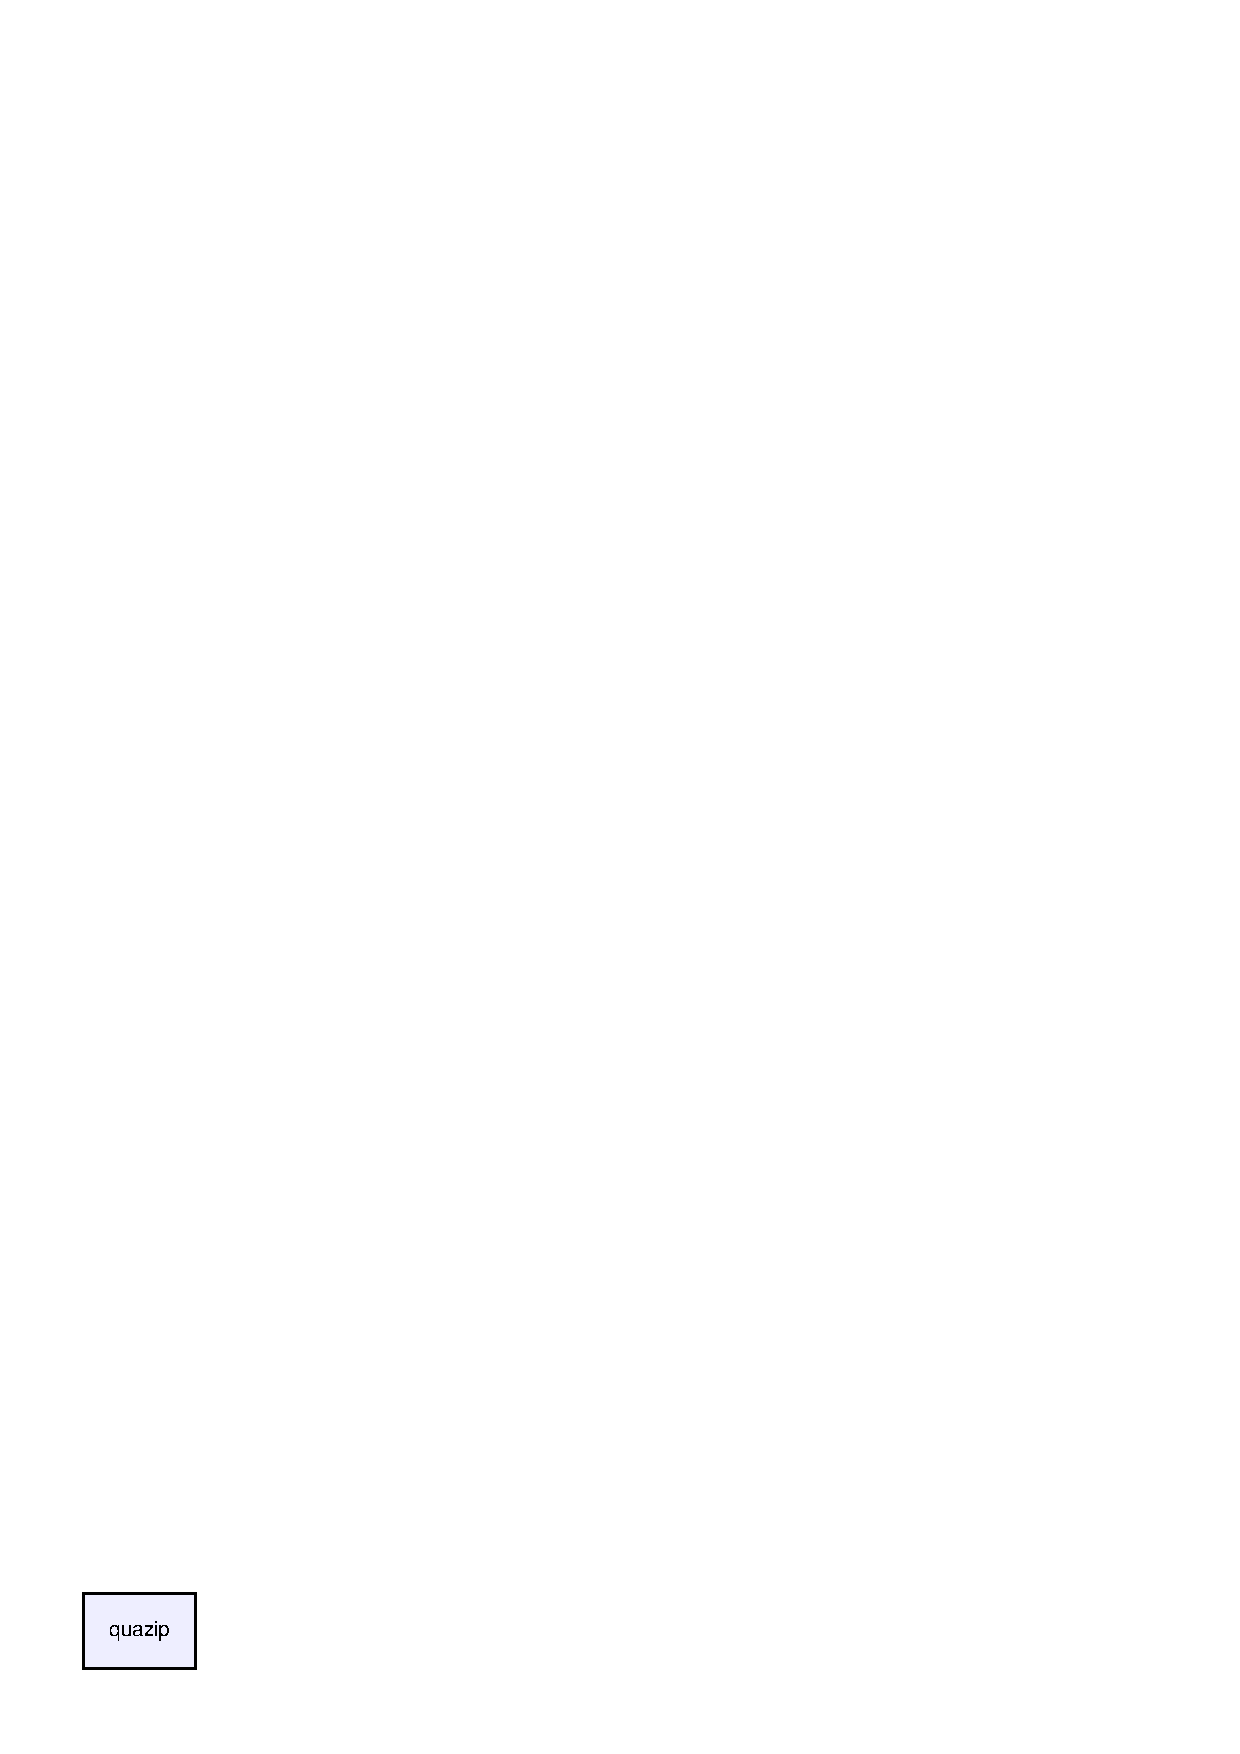
\includegraphics[width=98pt]{dir_e7d3eab1e7c75d6cf2e0a967be43a7d0_dep}
\end{center}
\end{figure}
\subsection*{Files}
\begin{DoxyCompactItemize}
\item 
file {\bfseries JlCompress.cpp}
\item 
file {\bfseries JlCompress.h}
\item 
file {\bfseries qioapi.cpp}
\item 
file {\bfseries quaadler32.cpp}
\item 
file {\bfseries quaadler32.h}
\item 
file {\bfseries quachecksum32.h}
\item 
file {\bfseries quacrc32.cpp}
\item 
file {\bfseries quacrc32.h}
\item 
file {\bfseries quagzipfile.cpp}
\item 
file {\bfseries quagzipfile.h}
\item 
file {\bfseries quaziodevice.cpp}
\item 
file {\bfseries quaziodevice.h}
\item 
file {\bfseries quazip.cpp}
\item 
file {\bfseries quazip.h}
\item 
file {\bfseries quazip\_\-global.h}
\item 
file {\bfseries quazipdir.cpp}
\item 
file {\bfseries quazipdir.h}
\item 
file {\bfseries quazipfile.cpp}
\item 
file {\bfseries quazipfile.h}
\item 
file {\bfseries quazipfileinfo.cpp}
\item 
file {\bfseries quazipfileinfo.h}
\item 
file {\bfseries quazipnewinfo.cpp}
\item 
file {\bfseries quazipnewinfo.h}
\end{DoxyCompactItemize}

\chapter{Class Documentation}
\section{JlCompress Class Reference}
\label{classJlCompress}\index{JlCompress@{JlCompress}}


Utility class for typical operations.  




{\ttfamily \#include $<$JlCompress.h$>$}

\subsection*{Static Public Member Functions}
\begin{DoxyCompactItemize}
\item 
static bool {\bf compressFile} ({\bf QString} fileCompressed, {\bf QString} file)
\begin{DoxyCompactList}\small\item\em Compress a single file. \end{DoxyCompactList}\item 
static bool {\bf compressFiles} ({\bf QString} fileCompressed, {\bf QStringList} files)
\begin{DoxyCompactList}\small\item\em Compress a list of files. \end{DoxyCompactList}\item 
static bool {\bf compressDir} ({\bf QString} fileCompressed, {\bf QString} dir={\bf QString}(), bool recursive=true)
\begin{DoxyCompactList}\small\item\em Compress a whole directory. \end{DoxyCompactList}\item 
static bool {\bf compressDir} ({\bf QString} fileCompressed, {\bf QString} dir, bool recursive, {\bf QDir::Filters} filters)
\begin{DoxyCompactList}\small\item\em Compress a whole directory. \end{DoxyCompactList}\item 
static {\bf QString} {\bf extractFile} ({\bf QString} fileCompressed, {\bf QString} fileName, {\bf QString} fileDest={\bf QString}())
\begin{DoxyCompactList}\small\item\em Extract a single file. \end{DoxyCompactList}\item 
static {\bf QStringList} {\bf extractFiles} ({\bf QString} fileCompressed, {\bf QStringList} files, {\bf QString} dir={\bf QString}())
\begin{DoxyCompactList}\small\item\em Extract a list of files. \end{DoxyCompactList}\item 
static {\bf QStringList} {\bf extractDir} ({\bf QString} fileCompressed, {\bf QString} dir={\bf QString}())
\begin{DoxyCompactList}\small\item\em Extract a whole archive. \end{DoxyCompactList}\item 
static {\bf QStringList} {\bf getFileList} ({\bf QString} fileCompressed)
\begin{DoxyCompactList}\small\item\em Get the file list. \end{DoxyCompactList}\item 
static {\bf QString} {\bf extractFile} ({\bf QIODevice} $\ast$ioDevice, {\bf QString} fileName, {\bf QString} fileDest={\bf QString}())
\begin{DoxyCompactList}\small\item\em Extract a single file. \end{DoxyCompactList}\item 
static {\bf QStringList} {\bf extractFiles} ({\bf QIODevice} $\ast$ioDevice, {\bf QStringList} files, {\bf QString} dir={\bf QString}())
\begin{DoxyCompactList}\small\item\em Extract a list of files. \end{DoxyCompactList}\item 
static {\bf QStringList} {\bf extractDir} ({\bf QIODevice} $\ast$ioDevice, {\bf QString} dir={\bf QString}())
\begin{DoxyCompactList}\small\item\em Extract a whole archive. \end{DoxyCompactList}\item 
static {\bf QStringList} {\bf getFileList} ({\bf QIODevice} $\ast$ioDevice)
\begin{DoxyCompactList}\small\item\em Get the file list. \end{DoxyCompactList}\end{DoxyCompactItemize}


\subsection{Detailed Description}
Utility class for typical operations. 

This class contains a number of useful static functions to perform simple operations, such as mass ZIP packing or extraction. 

\subsection{Member Function Documentation}
\index{JlCompress@{JlCompress}!compressFile@{compressFile}}
\index{compressFile@{compressFile}!JlCompress@{JlCompress}}
\subsubsection[{compressFile}]{\setlength{\rightskip}{0pt plus 5cm}bool JlCompress::compressFile (
\begin{DoxyParamCaption}
\item[{{\bf QString}}]{fileCompressed, }
\item[{{\bf QString}}]{file}
\end{DoxyParamCaption}
)\hspace{0.3cm}{\ttfamily  [static]}}\label{classJlCompress_a4a4de9c62ecf161bb658d4d80495ea97}


Compress a single file. 


\begin{DoxyParams}{Parameters}
{\em fileCompressed} & The name of the archive. \\
\hline
{\em file} & The file to compress. \\
\hline
\end{DoxyParams}
\begin{DoxyReturn}{Returns}
true if success, false otherwise. 
\end{DoxyReturn}


References QuaZip::close(), QuaZip::getZipError(), QuaZip::mdCreate, QDir::mkpath(), QuaZip::open(), and QFile::remove().

\index{JlCompress@{JlCompress}!compressFiles@{compressFiles}}
\index{compressFiles@{compressFiles}!JlCompress@{JlCompress}}
\subsubsection[{compressFiles}]{\setlength{\rightskip}{0pt plus 5cm}bool JlCompress::compressFiles (
\begin{DoxyParamCaption}
\item[{{\bf QString}}]{fileCompressed, }
\item[{{\bf QStringList}}]{files}
\end{DoxyParamCaption}
)\hspace{0.3cm}{\ttfamily  [static]}}\label{classJlCompress_a9cdb92d29a94c6b13a718a3249685846}


Compress a list of files. 


\begin{DoxyParams}{Parameters}
{\em fileCompressed} & The name of the archive. \\
\hline
{\em files} & The file list to compress. \\
\hline
\end{DoxyParams}
\begin{DoxyReturn}{Returns}
true if success, false otherwise. 
\end{DoxyReturn}


References QuaZip::close(), QFileInfo::exists(), QFileInfo::fileName(), QuaZip::getZipError(), QuaZip::mdCreate, QDir::mkpath(), QuaZip::open(), QFile::remove(), and QFileInfo::setFile().

\index{JlCompress@{JlCompress}!compressDir@{compressDir}}
\index{compressDir@{compressDir}!JlCompress@{JlCompress}}
\subsubsection[{compressDir}]{\setlength{\rightskip}{0pt plus 5cm}bool JlCompress::compressDir (
\begin{DoxyParamCaption}
\item[{{\bf QString}}]{fileCompressed, }
\item[{{\bf QString}}]{dir = {\ttfamily {\bf QString}()}, }
\item[{bool}]{recursive = {\ttfamily true}}
\end{DoxyParamCaption}
)\hspace{0.3cm}{\ttfamily  [static]}}\label{classJlCompress_a8708eafcadc5c192a1d492e784cfc98f}


Compress a whole directory. 

Does not compress hidden files. See \doxyref{compressDir(QString, QString, bool, QDir::Filters)}{p.}{classJlCompress_ada7511686a24c014e9db25735be148a7}.


\begin{DoxyParams}{Parameters}
{\em fileCompressed} & The name of the archive. \\
\hline
{\em dir} & The directory to compress. \\
\hline
{\em recursive} & Whether to pack the subdirectories as well, or just regular files. \\
\hline
\end{DoxyParams}
\begin{DoxyReturn}{Returns}
true if success, false otherwise. 
\end{DoxyReturn}
\index{JlCompress@{JlCompress}!compressDir@{compressDir}}
\index{compressDir@{compressDir}!JlCompress@{JlCompress}}
\subsubsection[{compressDir}]{\setlength{\rightskip}{0pt plus 5cm}bool JlCompress::compressDir (
\begin{DoxyParamCaption}
\item[{{\bf QString}}]{fileCompressed, }
\item[{{\bf QString}}]{dir, }
\item[{bool}]{recursive, }
\item[{{\bf QDir::Filters}}]{filters}
\end{DoxyParamCaption}
)\hspace{0.3cm}{\ttfamily  [static]}}\label{classJlCompress_ada7511686a24c014e9db25735be148a7}


Compress a whole directory. 

Unless filters are specified explicitly, packs only regular non-\/hidden files (and subdirs, if {\ttfamily recursive} is true). If filters are specified, they are OR-\/combined with {\ttfamily QDir::AllDirs$|$QDir::NoDotAndDotDot} when searching for dirs and with {\ttfamily QDir::Files} when searching for files.


\begin{DoxyParams}{Parameters}
{\em fileCompressed} & path to the resulting archive \\
\hline
{\em dir} & path to the directory being compressed \\
\hline
{\em recursive} & if true, then the subdirectories are packed as well \\
\hline
{\em filters} & what to pack, filters are applied both when searching for subdirs (if packing recursively) and when looking for files to pack \\
\hline
\end{DoxyParams}
\begin{DoxyReturn}{Returns}
true on success, false otherwise 
\end{DoxyReturn}


References QuaZip::close(), QuaZip::getZipError(), QuaZip::mdCreate, QDir::mkpath(), QuaZip::open(), and QFile::remove().

\index{JlCompress@{JlCompress}!extractFile@{extractFile}}
\index{extractFile@{extractFile}!JlCompress@{JlCompress}}
\subsubsection[{extractFile}]{\setlength{\rightskip}{0pt plus 5cm}{\bf QString} JlCompress::extractFile (
\begin{DoxyParamCaption}
\item[{{\bf QString}}]{fileCompressed, }
\item[{{\bf QString}}]{fileName, }
\item[{{\bf QString}}]{fileDest = {\ttfamily {\bf QString}()}}
\end{DoxyParamCaption}
)\hspace{0.3cm}{\ttfamily  [static]}}\label{classJlCompress_a38c0d58bfe3bbbcb3cf4e98d126633a3}


Extract a single file. 


\begin{DoxyParams}{Parameters}
{\em fileCompressed} & The name of the archive. \\
\hline
{\em fileName} & The file to extract. \\
\hline
{\em fileDest} & The destination file, assumed to be identical to {\itshape file\/} if left empty. \\
\hline
\end{DoxyParams}
\begin{DoxyReturn}{Returns}
The list of the full paths of the files extracted, empty on failure. 
\end{DoxyReturn}
\index{JlCompress@{JlCompress}!extractFiles@{extractFiles}}
\index{extractFiles@{extractFiles}!JlCompress@{JlCompress}}
\subsubsection[{extractFiles}]{\setlength{\rightskip}{0pt plus 5cm}{\bf QStringList} JlCompress::extractFiles (
\begin{DoxyParamCaption}
\item[{{\bf QString}}]{fileCompressed, }
\item[{{\bf QStringList}}]{files, }
\item[{{\bf QString}}]{dir = {\ttfamily {\bf QString}()}}
\end{DoxyParamCaption}
)\hspace{0.3cm}{\ttfamily  [static]}}\label{classJlCompress_a309e9ee366719a4d8aa28f837fab73ae}


Extract a list of files. 


\begin{DoxyParams}{Parameters}
{\em fileCompressed} & The name of the archive. \\
\hline
{\em files} & The file list to extract. \\
\hline
{\em dir} & The directory to put the files to, the current directory if left empty. \\
\hline
\end{DoxyParams}
\begin{DoxyReturn}{Returns}
The list of the full paths of the files extracted, empty on failure. 
\end{DoxyReturn}
\index{JlCompress@{JlCompress}!extractDir@{extractDir}}
\index{extractDir@{extractDir}!JlCompress@{JlCompress}}
\subsubsection[{extractDir}]{\setlength{\rightskip}{0pt plus 5cm}{\bf QStringList} JlCompress::extractDir (
\begin{DoxyParamCaption}
\item[{{\bf QString}}]{fileCompressed, }
\item[{{\bf QString}}]{dir = {\ttfamily {\bf QString}()}}
\end{DoxyParamCaption}
)\hspace{0.3cm}{\ttfamily  [static]}}\label{classJlCompress_a365a153baa4c11812d93cbca60b6a293}


Extract a whole archive. 


\begin{DoxyParams}{Parameters}
{\em fileCompressed} & The name of the archive. \\
\hline
{\em dir} & The directory to extract to, the current directory if left empty. \\
\hline
\end{DoxyParams}
\begin{DoxyReturn}{Returns}
The list of the full paths of the files extracted, empty on failure. 
\end{DoxyReturn}
\index{JlCompress@{JlCompress}!getFileList@{getFileList}}
\index{getFileList@{getFileList}!JlCompress@{JlCompress}}
\subsubsection[{getFileList}]{\setlength{\rightskip}{0pt plus 5cm}{\bf QStringList} JlCompress::getFileList (
\begin{DoxyParamCaption}
\item[{{\bf QString}}]{fileCompressed}
\end{DoxyParamCaption}
)\hspace{0.3cm}{\ttfamily  [static]}}\label{classJlCompress_ab42422be913f817d7e04c1b1cd5d0156}


Get the file list. 

\begin{DoxyReturn}{Returns}
The list of the files in the archive, or, more precisely, the list of the entries, including both files and directories if they are present separately. 
\end{DoxyReturn}
\index{JlCompress@{JlCompress}!extractFile@{extractFile}}
\index{extractFile@{extractFile}!JlCompress@{JlCompress}}
\subsubsection[{extractFile}]{\setlength{\rightskip}{0pt plus 5cm}{\bf QString} JlCompress::extractFile (
\begin{DoxyParamCaption}
\item[{{\bf QIODevice} $\ast$}]{ioDevice, }
\item[{{\bf QString}}]{fileName, }
\item[{{\bf QString}}]{fileDest = {\ttfamily {\bf QString}()}}
\end{DoxyParamCaption}
)\hspace{0.3cm}{\ttfamily  [static]}}\label{classJlCompress_ae789e7e744129a0429dc976fdcd33eac}


Extract a single file. 


\begin{DoxyParams}{Parameters}
{\em ioDevice} & pointer to device with compressed data. \\
\hline
{\em fileName} & The file to extract. \\
\hline
{\em fileDest} & The destination file, assumed to be identical to {\itshape file\/} if left empty. \\
\hline
\end{DoxyParams}
\begin{DoxyReturn}{Returns}
The list of the full paths of the files extracted, empty on failure. 
\end{DoxyReturn}
\index{JlCompress@{JlCompress}!extractFiles@{extractFiles}}
\index{extractFiles@{extractFiles}!JlCompress@{JlCompress}}
\subsubsection[{extractFiles}]{\setlength{\rightskip}{0pt plus 5cm}{\bf QStringList} JlCompress::extractFiles (
\begin{DoxyParamCaption}
\item[{{\bf QIODevice} $\ast$}]{ioDevice, }
\item[{{\bf QStringList}}]{files, }
\item[{{\bf QString}}]{dir = {\ttfamily {\bf QString}()}}
\end{DoxyParamCaption}
)\hspace{0.3cm}{\ttfamily  [static]}}\label{classJlCompress_a741646b1e2a922b3c48c2627fdc35f5b}


Extract a list of files. 


\begin{DoxyParams}{Parameters}
{\em ioDevice} & pointer to device with compressed data. \\
\hline
{\em files} & The file list to extract. \\
\hline
{\em dir} & The directory to put the files to, the current directory if left empty. \\
\hline
\end{DoxyParams}
\begin{DoxyReturn}{Returns}
The list of the full paths of the files extracted, empty on failure. 
\end{DoxyReturn}
\index{JlCompress@{JlCompress}!extractDir@{extractDir}}
\index{extractDir@{extractDir}!JlCompress@{JlCompress}}
\subsubsection[{extractDir}]{\setlength{\rightskip}{0pt plus 5cm}{\bf QStringList} JlCompress::extractDir (
\begin{DoxyParamCaption}
\item[{{\bf QIODevice} $\ast$}]{ioDevice, }
\item[{{\bf QString}}]{dir = {\ttfamily {\bf QString}()}}
\end{DoxyParamCaption}
)\hspace{0.3cm}{\ttfamily  [static]}}\label{classJlCompress_ac7877bcdf951d634cc2e1e6afe52e908}


Extract a whole archive. 


\begin{DoxyParams}{Parameters}
{\em ioDevice} & pointer to device with compressed data. \\
\hline
{\em dir} & The directory to extract to, the current directory if left empty. \\
\hline
\end{DoxyParams}
\begin{DoxyReturn}{Returns}
The list of the full paths of the files extracted, empty on failure. 
\end{DoxyReturn}
\index{JlCompress@{JlCompress}!getFileList@{getFileList}}
\index{getFileList@{getFileList}!JlCompress@{JlCompress}}
\subsubsection[{getFileList}]{\setlength{\rightskip}{0pt plus 5cm}{\bf QStringList} JlCompress::getFileList (
\begin{DoxyParamCaption}
\item[{{\bf QIODevice} $\ast$}]{ioDevice}
\end{DoxyParamCaption}
)\hspace{0.3cm}{\ttfamily  [static]}}\label{classJlCompress_a4ae5501a229d15f228cc034fc97cf78d}


Get the file list. 

\begin{DoxyReturn}{Returns}
The list of the files in the archive, or, more precisely, the list of the entries, including both files and directories if they are present separately. 
\end{DoxyReturn}


The documentation for this class was generated from the following files:\begin{DoxyCompactItemize}
\item 
quazip/JlCompress.h\item 
quazip/JlCompress.cpp\end{DoxyCompactItemize}

\section{QuaAdler32 Class Reference}
\label{classQuaAdler32}\index{QuaAdler32@{QuaAdler32}}


Adler32 checksum.  




{\ttfamily \#include $<$quazip/quaadler32.h$>$}



Inheritance diagram for QuaAdler32:
\nopagebreak
\begin{figure}[H]
\begin{center}
\leavevmode
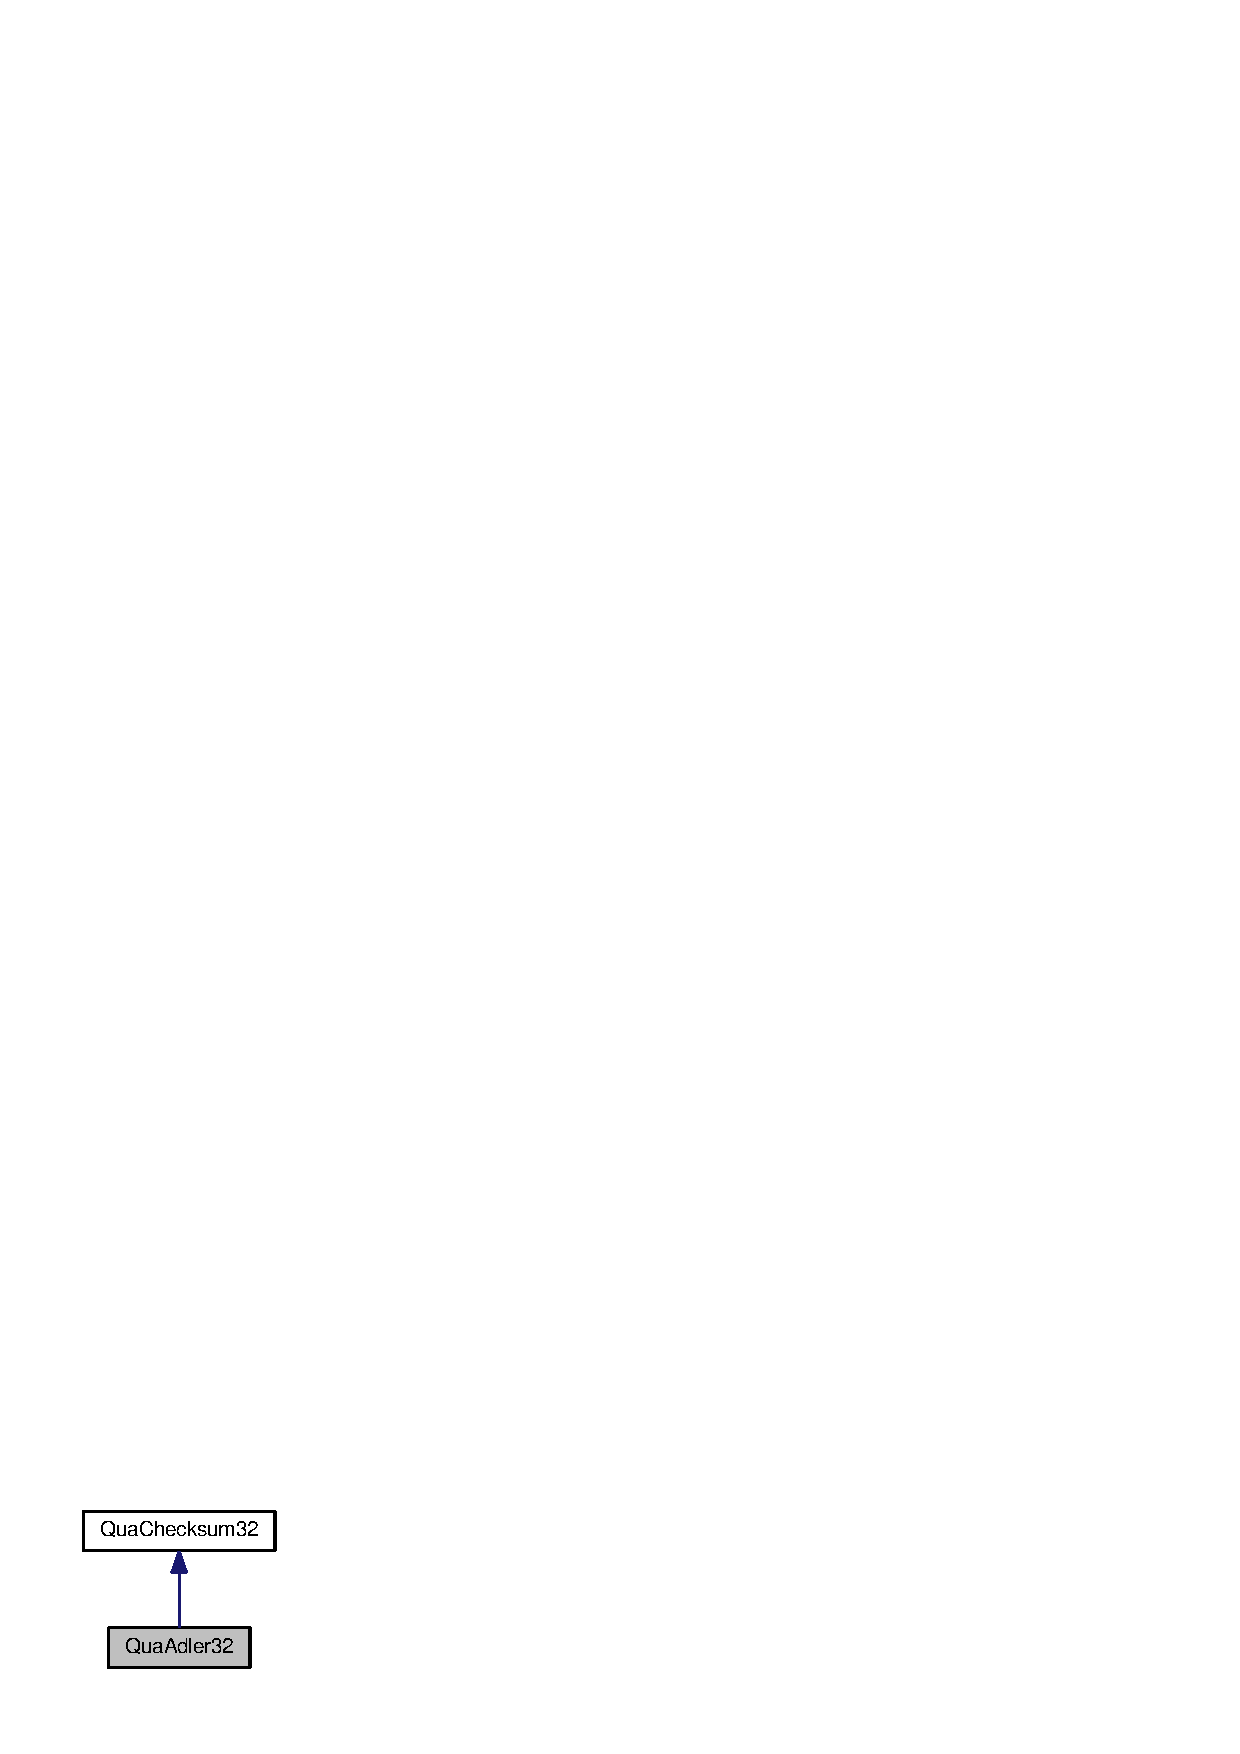
\includegraphics[width=136pt]{classQuaAdler32__inherit__graph}
\end{center}
\end{figure}


Collaboration diagram for QuaAdler32:
\nopagebreak
\begin{figure}[H]
\begin{center}
\leavevmode
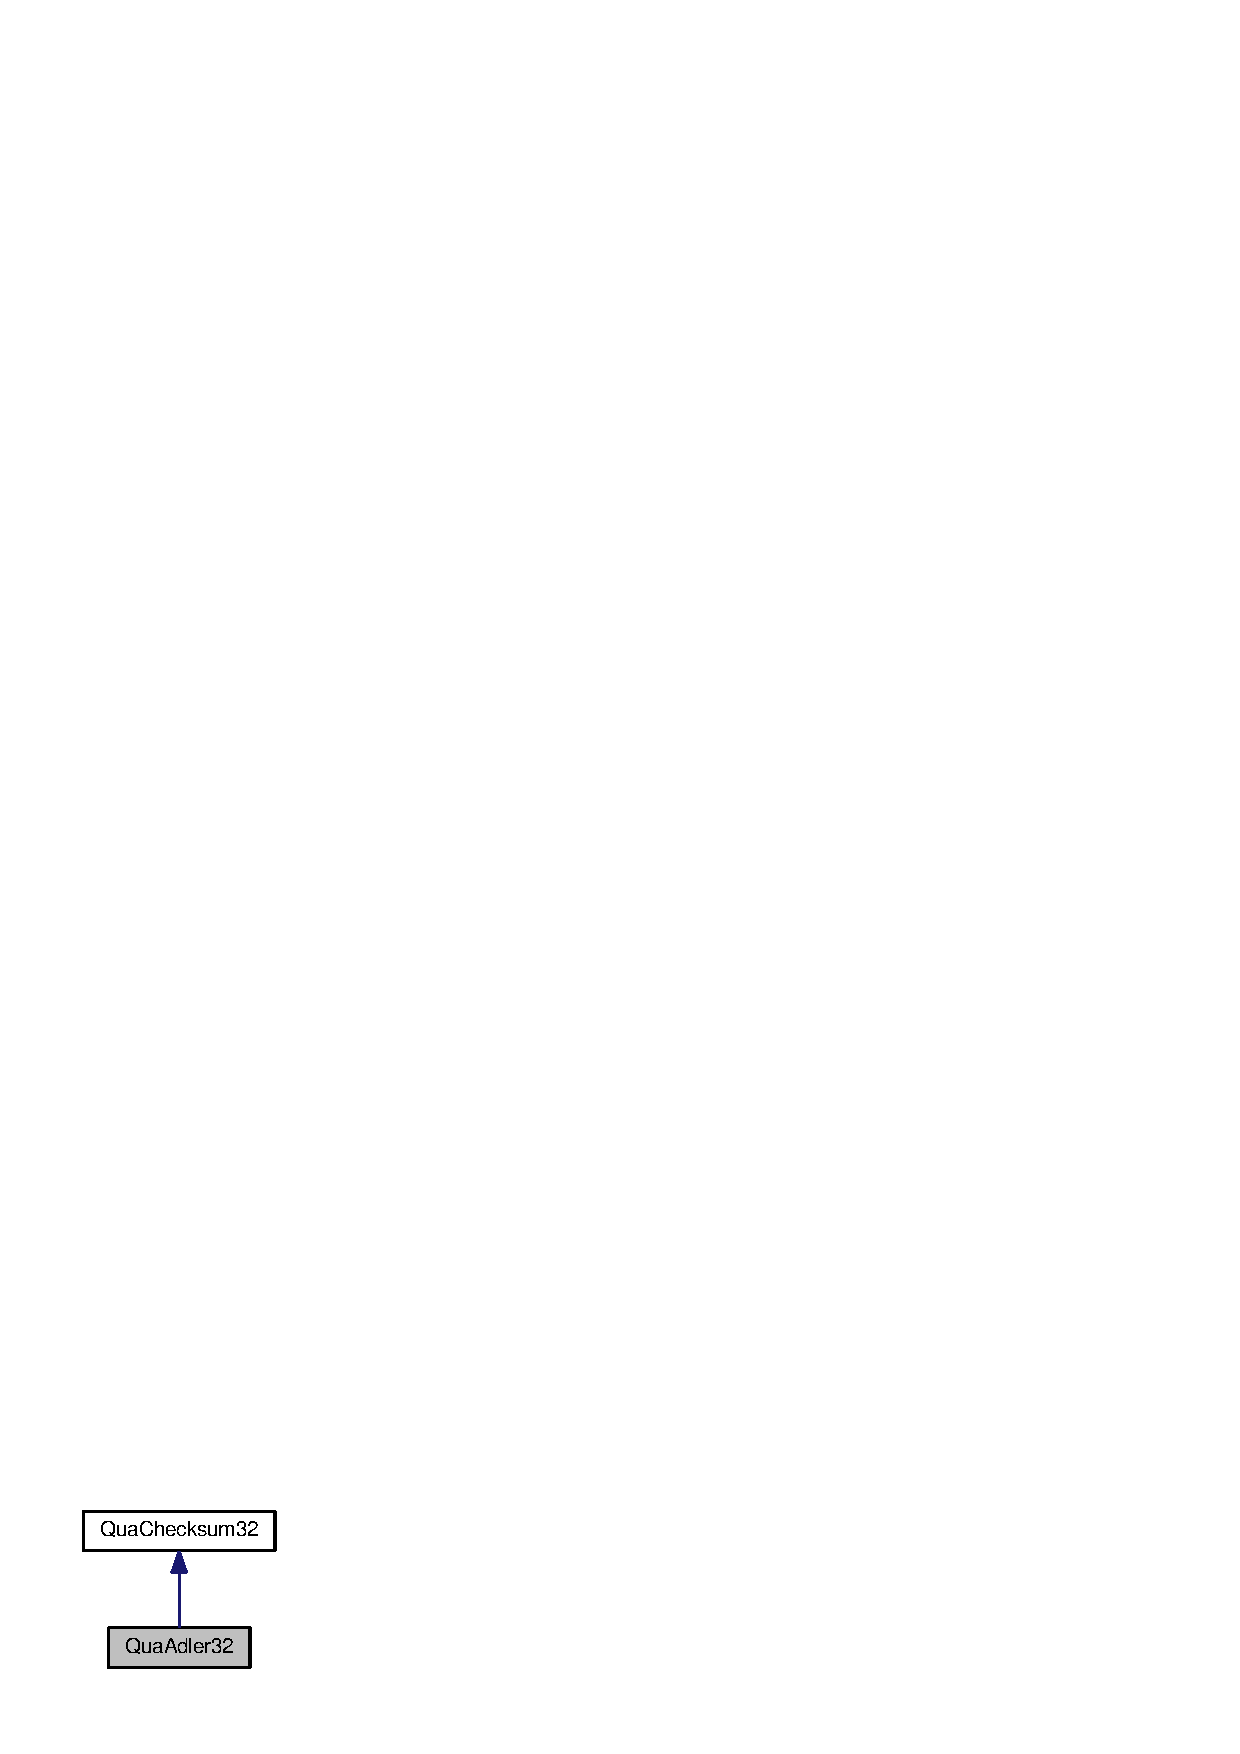
\includegraphics[width=136pt]{classQuaAdler32__coll__graph}
\end{center}
\end{figure}
\subsection*{Public Member Functions}
\begin{DoxyCompactItemize}
\item 
quint32 {\bf calculate} (const {\bf QByteArray} \&data)
\begin{DoxyCompactList}\small\item\em Calculates the checksum for data. \end{DoxyCompactList}\item 
void {\bf reset} ()\label{classQuaAdler32_a2fe6ac9eb289bafda6a9fd20e6472ab5}

\begin{DoxyCompactList}\small\item\em Resets the calculation on a checksun for a stream. \end{DoxyCompactList}\item 
void {\bf update} (const {\bf QByteArray} \&buf)
\begin{DoxyCompactList}\small\item\em Updates the calculated checksum for the stream. \end{DoxyCompactList}\item 
quint32 {\bf value} ()
\begin{DoxyCompactList}\small\item\em Value of the checksum calculated for the stream passed throw \doxyref{update()}{p.}{classQuaAdler32_aba24f7b16aa0cdc26f81a9ad687fc653}. \end{DoxyCompactList}\end{DoxyCompactItemize}


\subsection{Detailed Description}
Adler32 checksum. 

This class wrappers the adler32 function with the \doxyref{QuaChecksum32}{p.}{classQuaChecksum32} interface. See \doxyref{QuaChecksum32}{p.}{classQuaChecksum32} for more info. 

\subsection{Member Function Documentation}
\index{QuaAdler32@{QuaAdler32}!calculate@{calculate}}
\index{calculate@{calculate}!QuaAdler32@{QuaAdler32}}
\subsubsection[{calculate}]{\setlength{\rightskip}{0pt plus 5cm}quint32 QuaAdler32::calculate (
\begin{DoxyParamCaption}
\item[{const {\bf QByteArray} \&}]{data}
\end{DoxyParamCaption}
)\hspace{0.3cm}{\ttfamily  [virtual]}}\label{classQuaAdler32_a350e84fd000ebfa3c33503336a7b21bb}


Calculates the checksum for data. 

{\itshape data\/} source data \begin{DoxyReturn}{Returns}
data checksum
\end{DoxyReturn}
This function has no efect on the value returned by \doxyref{value()}{p.}{classQuaAdler32_a2022e1db95c23cef220b335e44d74fb1}. 

Implements {\bf QuaChecksum32} \doxyref{}{p.}{classQuaChecksum32_a14d800fcfd55b2ae11ef07d3924fe0b1}.



References QByteArray::data(), and QByteArray::size().

\index{QuaAdler32@{QuaAdler32}!update@{update}}
\index{update@{update}!QuaAdler32@{QuaAdler32}}
\subsubsection[{update}]{\setlength{\rightskip}{0pt plus 5cm}void QuaAdler32::update (
\begin{DoxyParamCaption}
\item[{const {\bf QByteArray} \&}]{buf}
\end{DoxyParamCaption}
)\hspace{0.3cm}{\ttfamily  [virtual]}}\label{classQuaAdler32_aba24f7b16aa0cdc26f81a9ad687fc653}


Updates the calculated checksum for the stream. 

{\itshape buf\/} next portion of data from the stream 

Implements {\bf QuaChecksum32} \doxyref{}{p.}{classQuaChecksum32_a63a6ed3171f9243214d307da67557f7e}.



References QByteArray::data(), and QByteArray::size().

\index{QuaAdler32@{QuaAdler32}!value@{value}}
\index{value@{value}!QuaAdler32@{QuaAdler32}}
\subsubsection[{value}]{\setlength{\rightskip}{0pt plus 5cm}quint32 QuaAdler32::value (
\begin{DoxyParamCaption}
{}
\end{DoxyParamCaption}
)\hspace{0.3cm}{\ttfamily  [virtual]}}\label{classQuaAdler32_a2022e1db95c23cef220b335e44d74fb1}


Value of the checksum calculated for the stream passed throw \doxyref{update()}{p.}{classQuaAdler32_aba24f7b16aa0cdc26f81a9ad687fc653}. 

\begin{DoxyReturn}{Returns}
checksum 
\end{DoxyReturn}


Implements {\bf QuaChecksum32} \doxyref{}{p.}{classQuaChecksum32_afd836e7534194fce08356be6a8336da7}.



The documentation for this class was generated from the following files:\begin{DoxyCompactItemize}
\item 
quazip/quaadler32.h\item 
quazip/quaadler32.cpp\end{DoxyCompactItemize}

\section{QuaChecksum32 Class Reference}
\label{classQuaChecksum32}\index{QuaChecksum32@{QuaChecksum32}}


Checksum interface.  




{\ttfamily \#include $<$quazip/quachecksum32.h$>$}



Inheritance diagram for QuaChecksum32:
\nopagebreak
\begin{figure}[H]
\begin{center}
\leavevmode
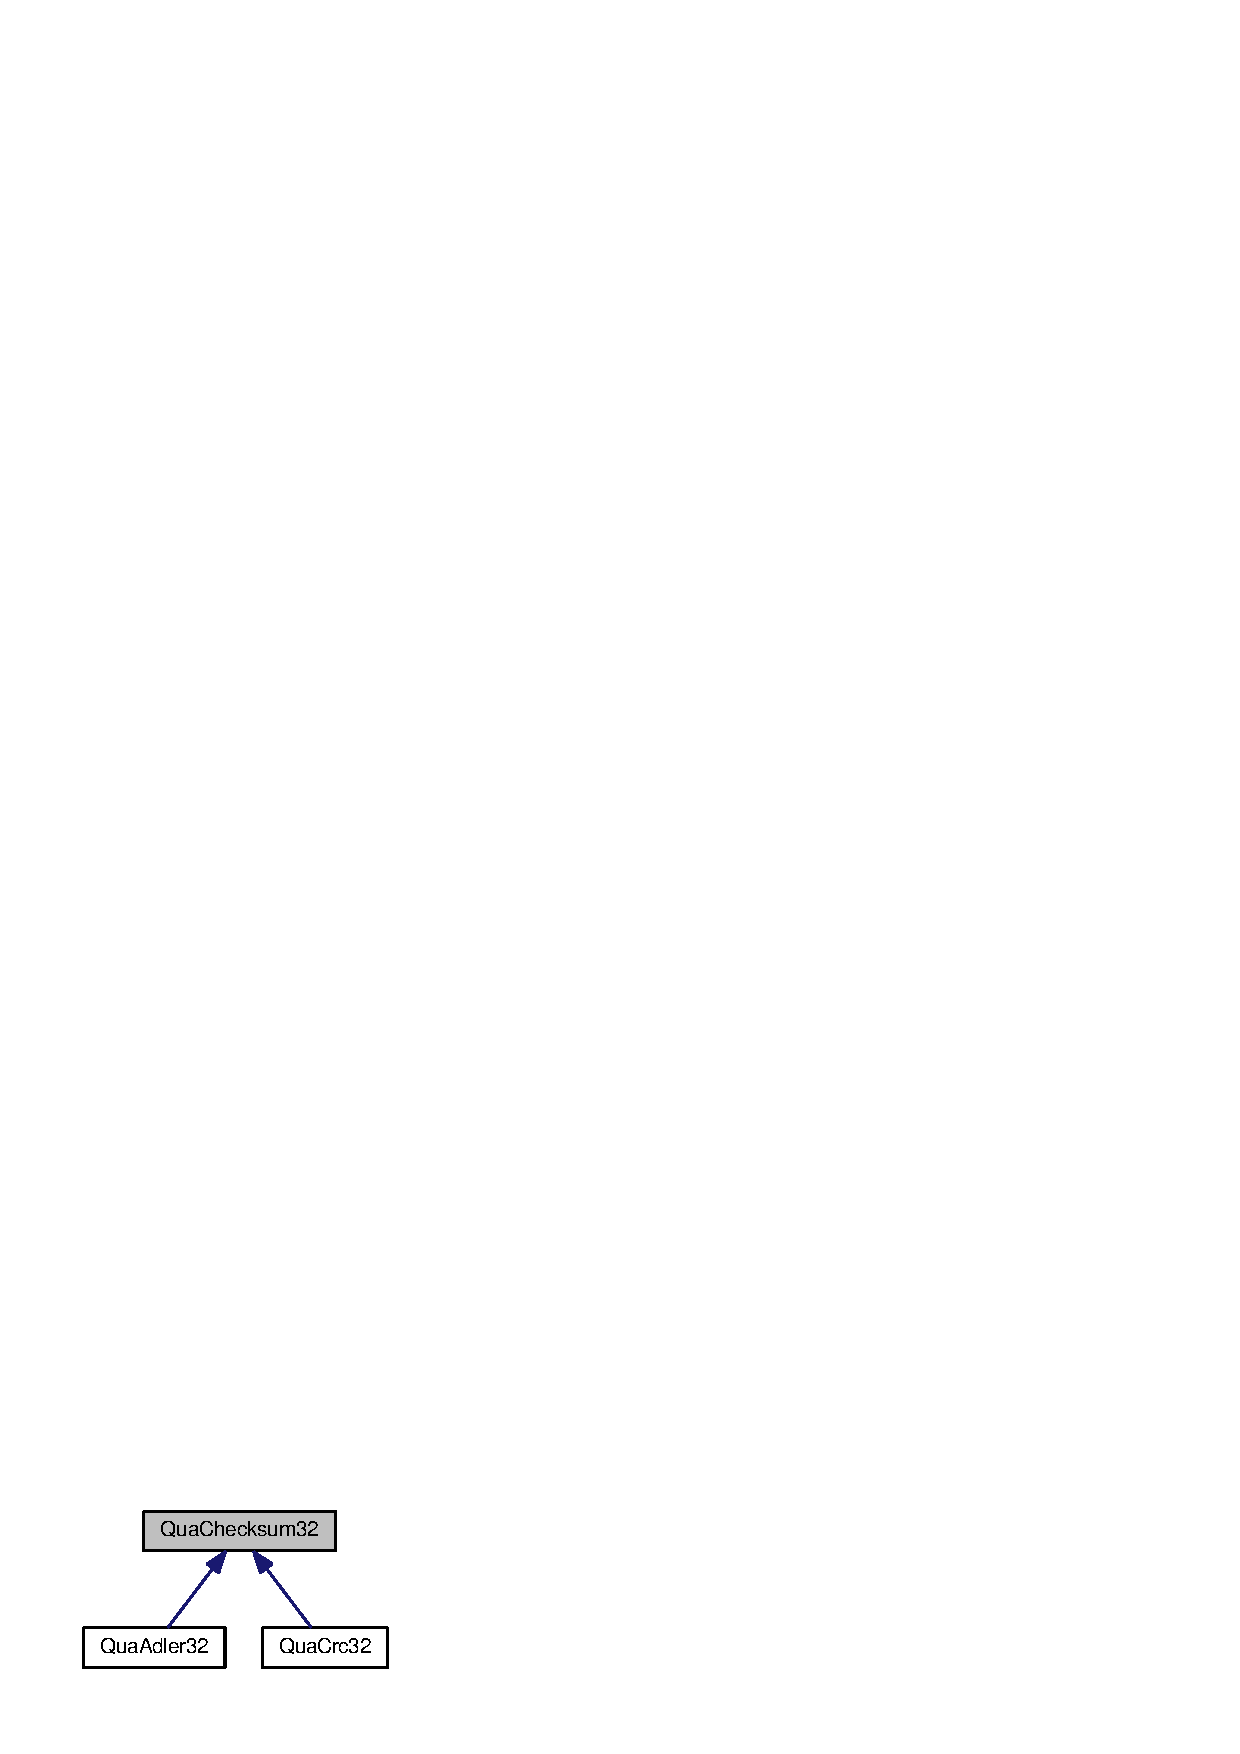
\includegraphics[width=190pt]{classQuaChecksum32__inherit__graph}
\end{center}
\end{figure}
\subsection*{Public Member Functions}
\begin{DoxyCompactItemize}
\item 
virtual quint32 {\bf calculate} (const {\bf QByteArray} \&data)=0
\begin{DoxyCompactList}\small\item\em Calculates the checksum for data. \end{DoxyCompactList}\item 
virtual void {\bf reset} ()=0\label{classQuaChecksum32_ad3f5db3c76b00069db9bda333cb49d57}

\begin{DoxyCompactList}\small\item\em Resets the calculation on a checksun for a stream. \end{DoxyCompactList}\item 
virtual void {\bf update} (const {\bf QByteArray} \&buf)=0
\begin{DoxyCompactList}\small\item\em Updates the calculated checksum for the stream. \end{DoxyCompactList}\item 
virtual quint32 {\bf value} ()=0
\begin{DoxyCompactList}\small\item\em Value of the checksum calculated for the stream passed throw \doxyref{update()}{p.}{classQuaChecksum32_a63a6ed3171f9243214d307da67557f7e}. \end{DoxyCompactList}\end{DoxyCompactItemize}


\subsection{Detailed Description}
Checksum interface. 

This is an interface for 32 bit checksums. Classes implementing this interface can calcunate a certin checksum in a single step: 
\begin{DoxyCode}
 QChecksum32 *crc32 = new QuaCrc32(); 
 rasoult = crc32->calculate(data);
\end{DoxyCode}
 or by streaming the data: 
\begin{DoxyCode}
 QChecksum32 *crc32 = new QuaCrc32(); 
 while(!fileA.atEnd())
     crc32->update(fileA.read(bufSize));
 resoultA = crc32->value();
 crc32->reset();
 while(!fileB.atEnd())
     crc32->update(fileB.read(bufSize));
 resoultB = crc32->value();
\end{DoxyCode}
 

\subsection{Member Function Documentation}
\index{QuaChecksum32@{QuaChecksum32}!calculate@{calculate}}
\index{calculate@{calculate}!QuaChecksum32@{QuaChecksum32}}
\subsubsection[{calculate}]{\setlength{\rightskip}{0pt plus 5cm}virtual quint32 QuaChecksum32::calculate (
\begin{DoxyParamCaption}
\item[{const {\bf QByteArray} \&}]{data}
\end{DoxyParamCaption}
)\hspace{0.3cm}{\ttfamily  [pure virtual]}}\label{classQuaChecksum32_a14d800fcfd55b2ae11ef07d3924fe0b1}


Calculates the checksum for data. 

{\itshape data\/} source data \begin{DoxyReturn}{Returns}
data checksum
\end{DoxyReturn}
This function has no efect on the value returned by \doxyref{value()}{p.}{classQuaChecksum32_afd836e7534194fce08356be6a8336da7}. 

Implemented in {\bf QuaAdler32} \doxyref{}{p.}{classQuaAdler32_a350e84fd000ebfa3c33503336a7b21bb}, and {\bf QuaCrc32} \doxyref{}{p.}{classQuaCrc32_aaf6fdf6e36e55c97bf9eab6ec65ecb9e}.

\index{QuaChecksum32@{QuaChecksum32}!update@{update}}
\index{update@{update}!QuaChecksum32@{QuaChecksum32}}
\subsubsection[{update}]{\setlength{\rightskip}{0pt plus 5cm}virtual void QuaChecksum32::update (
\begin{DoxyParamCaption}
\item[{const {\bf QByteArray} \&}]{buf}
\end{DoxyParamCaption}
)\hspace{0.3cm}{\ttfamily  [pure virtual]}}\label{classQuaChecksum32_a63a6ed3171f9243214d307da67557f7e}


Updates the calculated checksum for the stream. 

{\itshape buf\/} next portion of data from the stream 

Implemented in {\bf QuaAdler32} \doxyref{}{p.}{classQuaAdler32_aba24f7b16aa0cdc26f81a9ad687fc653}, and {\bf QuaCrc32} \doxyref{}{p.}{classQuaCrc32_a5015d80e04afe6e6d094155b7e99888e}.

\index{QuaChecksum32@{QuaChecksum32}!value@{value}}
\index{value@{value}!QuaChecksum32@{QuaChecksum32}}
\subsubsection[{value}]{\setlength{\rightskip}{0pt plus 5cm}virtual quint32 QuaChecksum32::value (
\begin{DoxyParamCaption}
{}
\end{DoxyParamCaption}
)\hspace{0.3cm}{\ttfamily  [pure virtual]}}\label{classQuaChecksum32_afd836e7534194fce08356be6a8336da7}


Value of the checksum calculated for the stream passed throw \doxyref{update()}{p.}{classQuaChecksum32_a63a6ed3171f9243214d307da67557f7e}. 

\begin{DoxyReturn}{Returns}
checksum 
\end{DoxyReturn}


Implemented in {\bf QuaAdler32} \doxyref{}{p.}{classQuaAdler32_a2022e1db95c23cef220b335e44d74fb1}, and {\bf QuaCrc32} \doxyref{}{p.}{classQuaCrc32_a957ce46a53862f75c89d6a3ac4f73389}.



The documentation for this class was generated from the following file:\begin{DoxyCompactItemize}
\item 
quazip/quachecksum32.h\end{DoxyCompactItemize}

\section{QuaCrc32 Class Reference}
\label{classQuaCrc32}\index{QuaCrc32@{QuaCrc32}}


CRC32 checksum.  




{\ttfamily \#include $<$quazip/quacrc32.h$>$}



Inheritance diagram for QuaCrc32:
\nopagebreak
\begin{figure}[H]
\begin{center}
\leavevmode
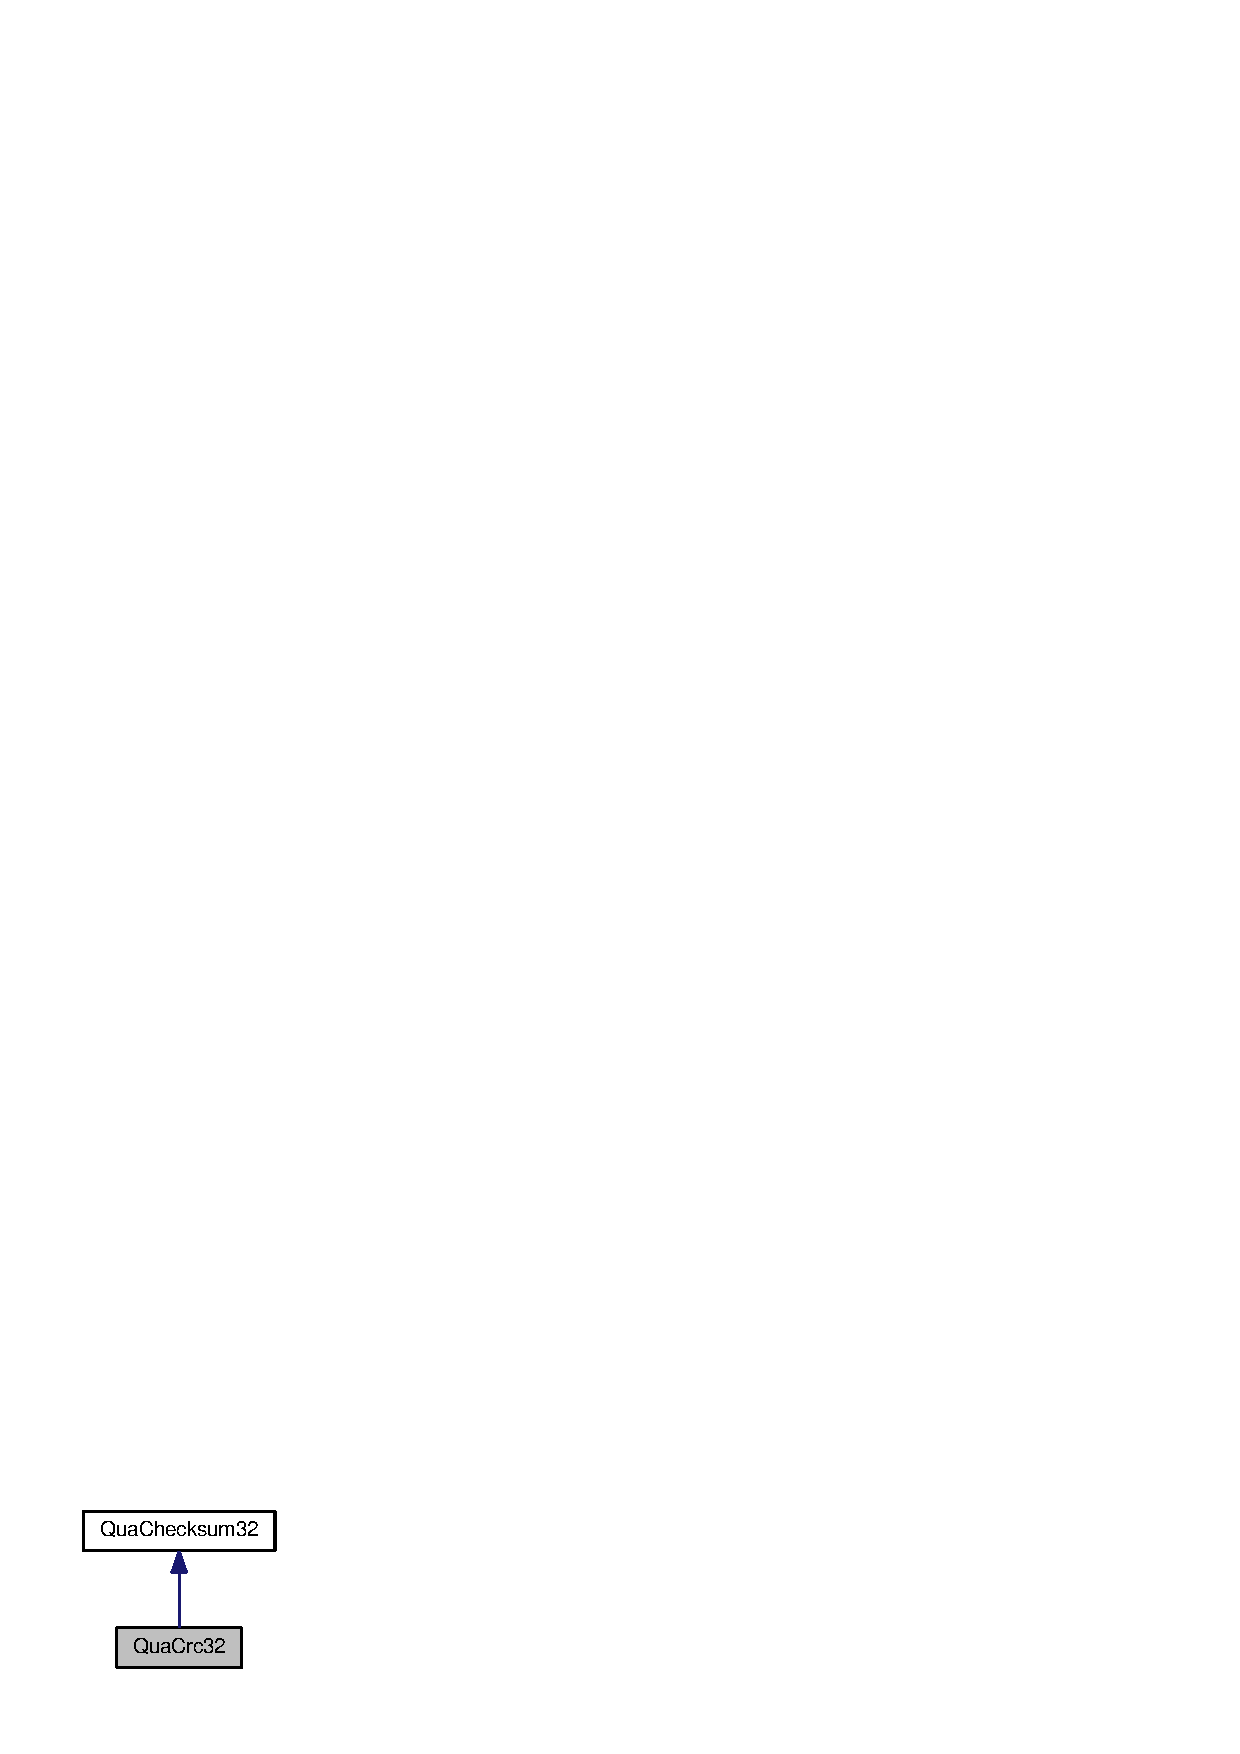
\includegraphics[width=136pt]{classQuaCrc32__inherit__graph}
\end{center}
\end{figure}


Collaboration diagram for QuaCrc32:
\nopagebreak
\begin{figure}[H]
\begin{center}
\leavevmode
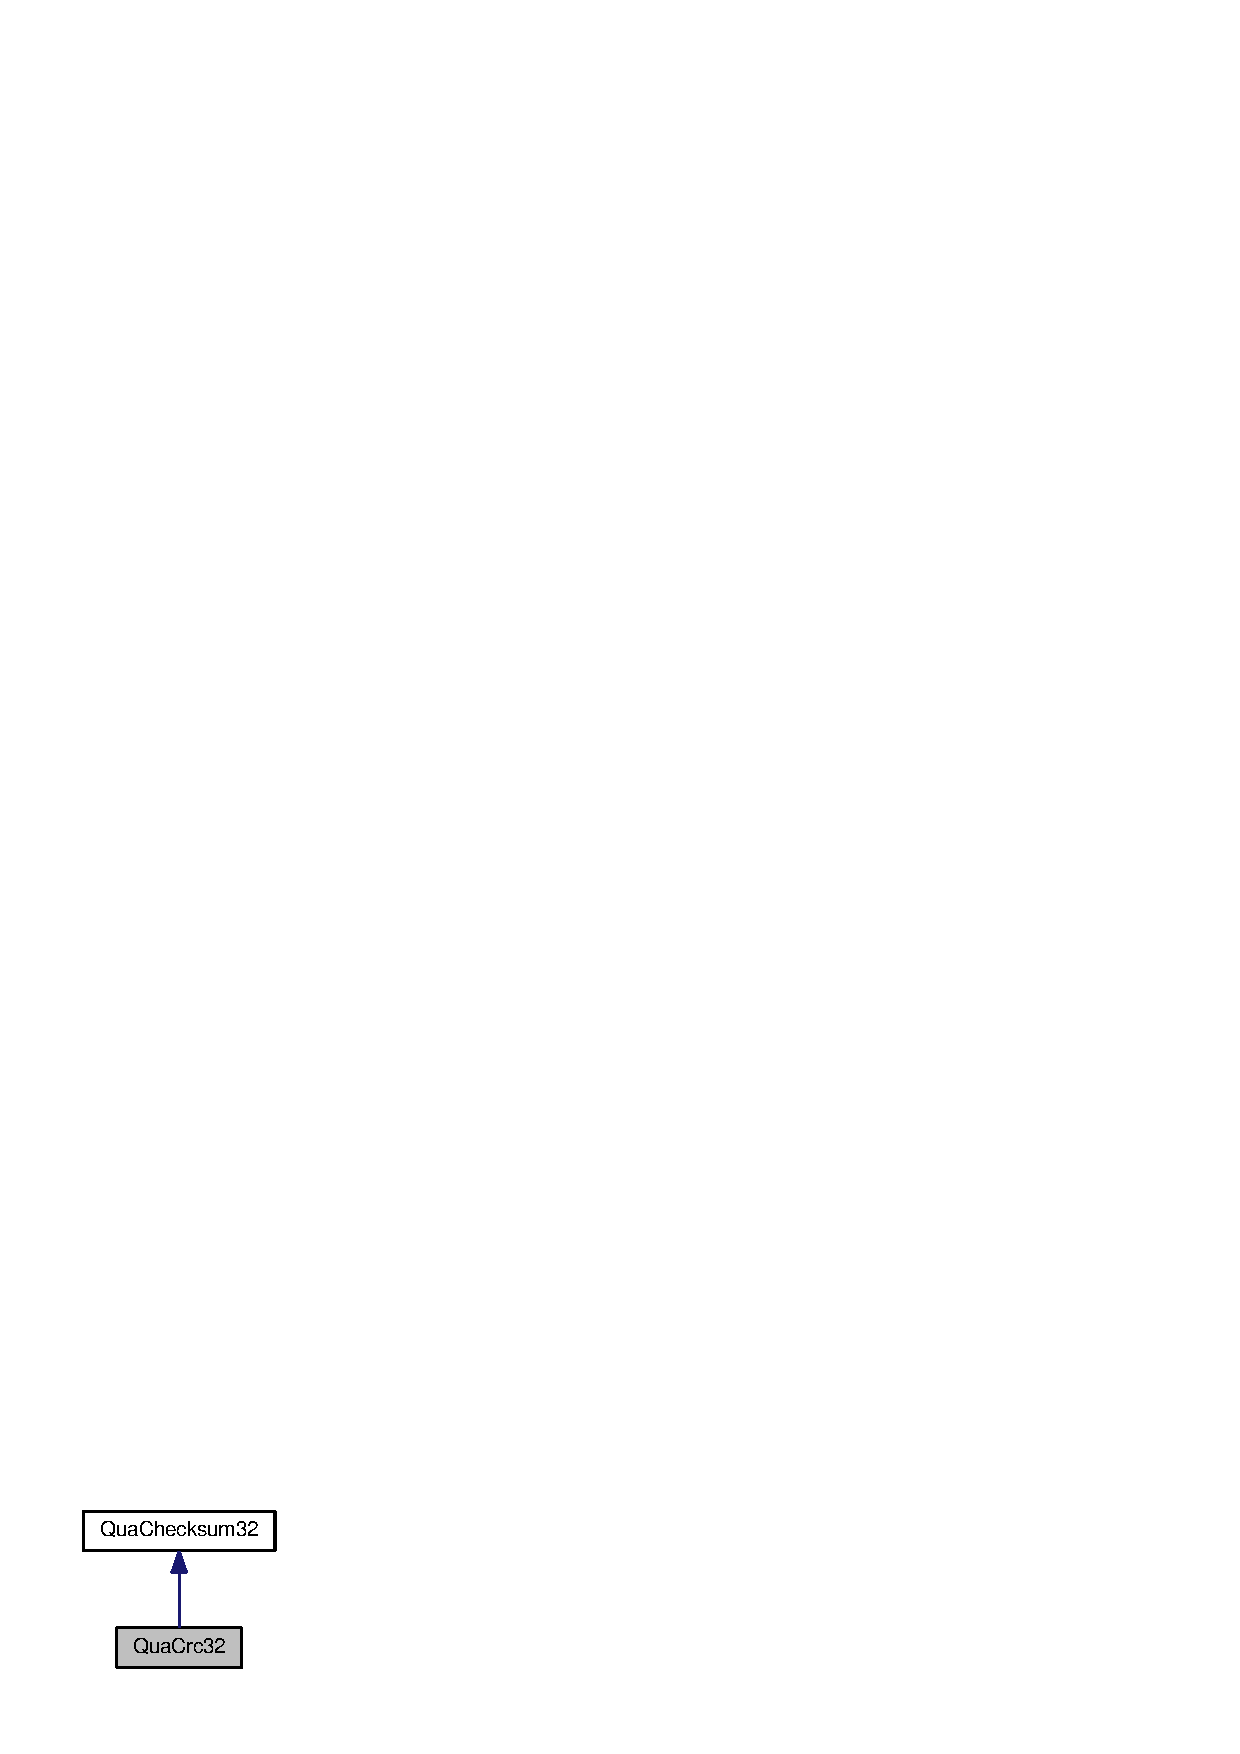
\includegraphics[width=136pt]{classQuaCrc32__coll__graph}
\end{center}
\end{figure}
\subsection*{Public Member Functions}
\begin{DoxyCompactItemize}
\item 
quint32 {\bf calculate} (const {\bf QByteArray} \&data)
\begin{DoxyCompactList}\small\item\em Calculates the checksum for data. \end{DoxyCompactList}\item 
void {\bf reset} ()\label{classQuaCrc32_a3fe7ce6cb73512c963ffaabfbbc66363}

\begin{DoxyCompactList}\small\item\em Resets the calculation on a checksun for a stream. \end{DoxyCompactList}\item 
void {\bf update} (const {\bf QByteArray} \&buf)
\begin{DoxyCompactList}\small\item\em Updates the calculated checksum for the stream. \end{DoxyCompactList}\item 
quint32 {\bf value} ()
\begin{DoxyCompactList}\small\item\em Value of the checksum calculated for the stream passed throw \doxyref{update()}{p.}{classQuaCrc32_a5015d80e04afe6e6d094155b7e99888e}. \end{DoxyCompactList}\end{DoxyCompactItemize}


\subsection{Detailed Description}
CRC32 checksum. 

This class wrappers the crc32 function with the \doxyref{QuaChecksum32}{p.}{classQuaChecksum32} interface. See \doxyref{QuaChecksum32}{p.}{classQuaChecksum32} for more info. 

\subsection{Member Function Documentation}
\index{QuaCrc32@{QuaCrc32}!calculate@{calculate}}
\index{calculate@{calculate}!QuaCrc32@{QuaCrc32}}
\subsubsection[{calculate}]{\setlength{\rightskip}{0pt plus 5cm}quint32 QuaCrc32::calculate (
\begin{DoxyParamCaption}
\item[{const {\bf QByteArray} \&}]{data}
\end{DoxyParamCaption}
)\hspace{0.3cm}{\ttfamily  [virtual]}}\label{classQuaCrc32_aaf6fdf6e36e55c97bf9eab6ec65ecb9e}


Calculates the checksum for data. 

{\itshape data\/} source data \begin{DoxyReturn}{Returns}
data checksum
\end{DoxyReturn}
This function has no efect on the value returned by \doxyref{value()}{p.}{classQuaCrc32_a957ce46a53862f75c89d6a3ac4f73389}. 

Implements {\bf QuaChecksum32} \doxyref{}{p.}{classQuaChecksum32_a14d800fcfd55b2ae11ef07d3924fe0b1}.



References QByteArray::data(), and QByteArray::size().

\index{QuaCrc32@{QuaCrc32}!update@{update}}
\index{update@{update}!QuaCrc32@{QuaCrc32}}
\subsubsection[{update}]{\setlength{\rightskip}{0pt plus 5cm}void QuaCrc32::update (
\begin{DoxyParamCaption}
\item[{const {\bf QByteArray} \&}]{buf}
\end{DoxyParamCaption}
)\hspace{0.3cm}{\ttfamily  [virtual]}}\label{classQuaCrc32_a5015d80e04afe6e6d094155b7e99888e}


Updates the calculated checksum for the stream. 

{\itshape buf\/} next portion of data from the stream 

Implements {\bf QuaChecksum32} \doxyref{}{p.}{classQuaChecksum32_a63a6ed3171f9243214d307da67557f7e}.



References QByteArray::data(), and QByteArray::size().

\index{QuaCrc32@{QuaCrc32}!value@{value}}
\index{value@{value}!QuaCrc32@{QuaCrc32}}
\subsubsection[{value}]{\setlength{\rightskip}{0pt plus 5cm}quint32 QuaCrc32::value (
\begin{DoxyParamCaption}
{}
\end{DoxyParamCaption}
)\hspace{0.3cm}{\ttfamily  [virtual]}}\label{classQuaCrc32_a957ce46a53862f75c89d6a3ac4f73389}


Value of the checksum calculated for the stream passed throw \doxyref{update()}{p.}{classQuaCrc32_a5015d80e04afe6e6d094155b7e99888e}. 

\begin{DoxyReturn}{Returns}
checksum 
\end{DoxyReturn}


Implements {\bf QuaChecksum32} \doxyref{}{p.}{classQuaChecksum32_afd836e7534194fce08356be6a8336da7}.



The documentation for this class was generated from the following files:\begin{DoxyCompactItemize}
\item 
quazip/quacrc32.h\item 
quazip/quacrc32.cpp\end{DoxyCompactItemize}

\section{QuaGzipFile Class Reference}
\label{classQuaGzipFile}\index{QuaGzipFile@{QuaGzipFile}}


GZIP file.  




{\ttfamily \#include $<$quagzipfile.h$>$}



Inheritance diagram for QuaGzipFile:
\nopagebreak
\begin{figure}[H]
\begin{center}
\leavevmode
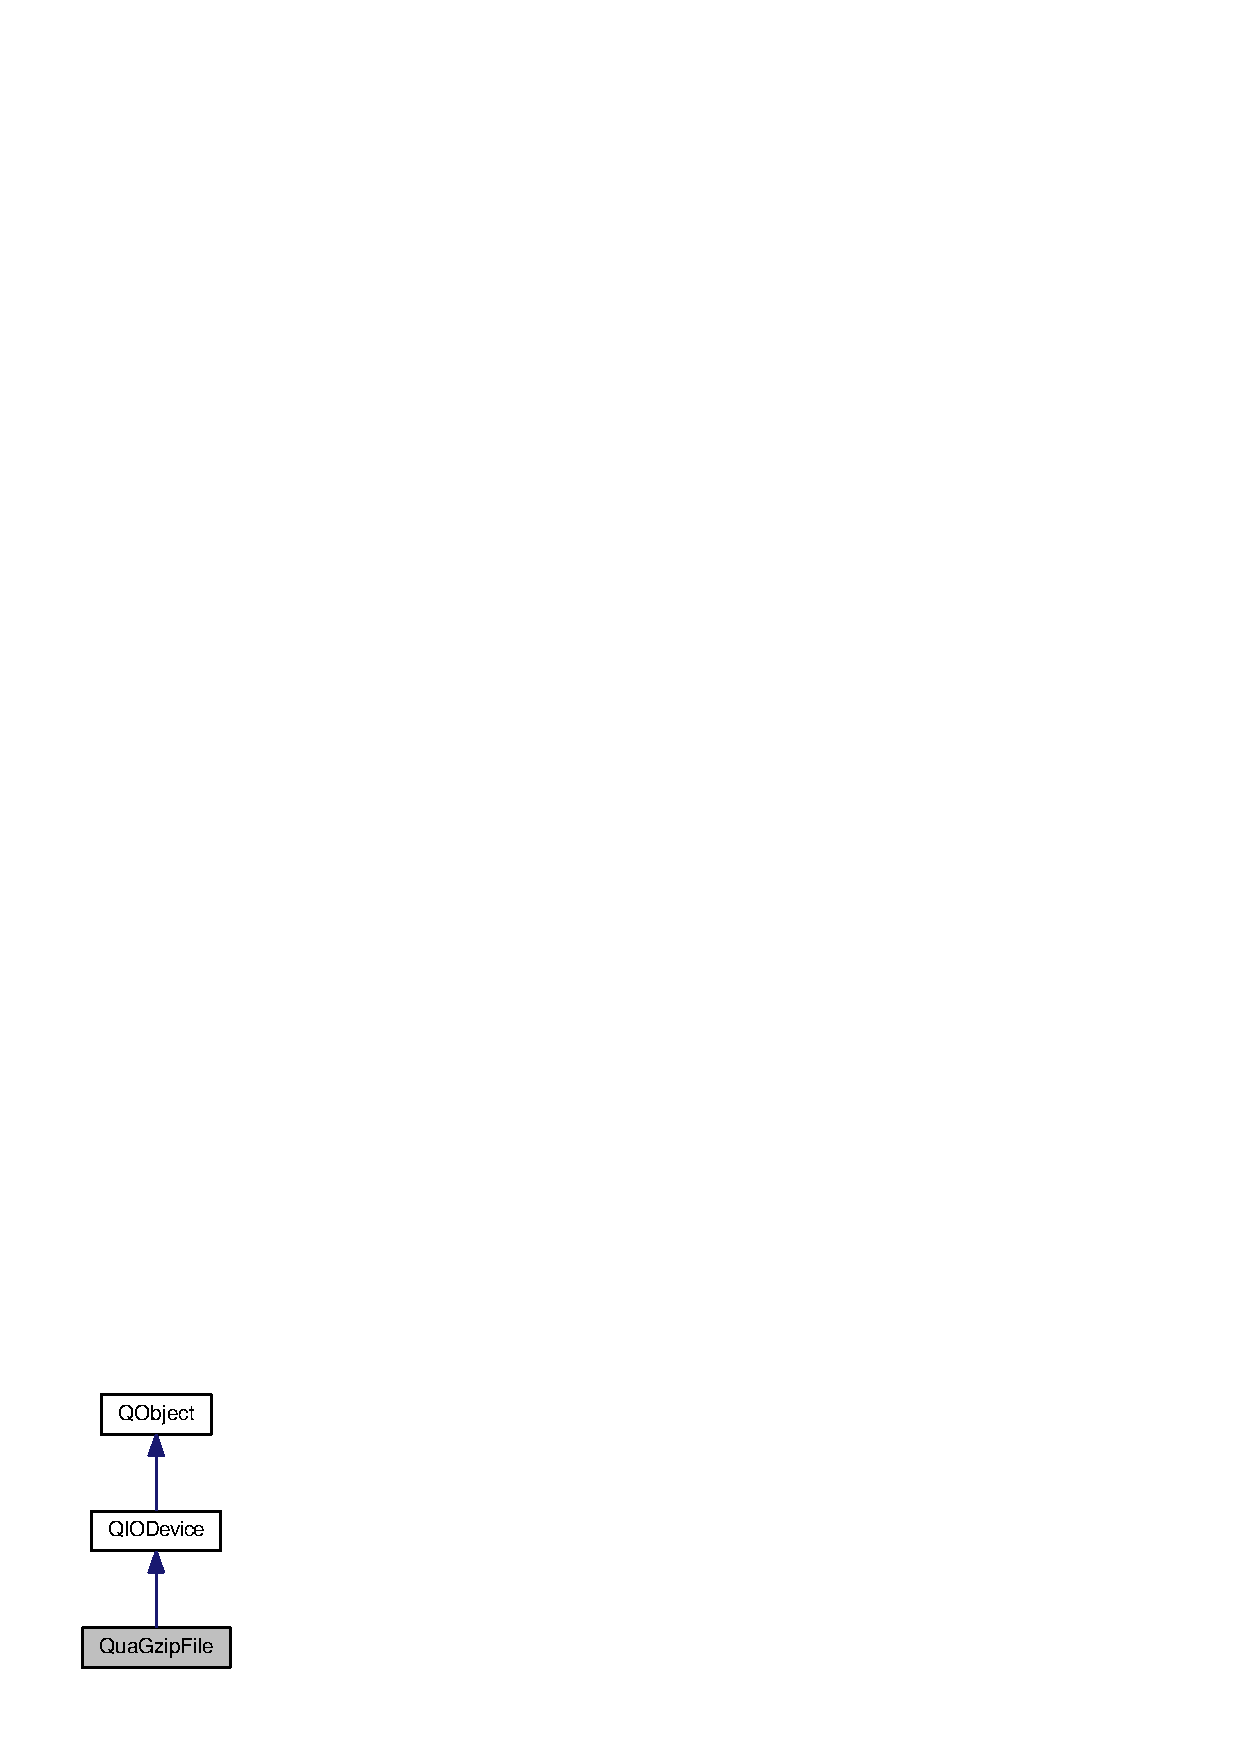
\includegraphics[width=114pt]{classQuaGzipFile__inherit__graph}
\end{center}
\end{figure}


Collaboration diagram for QuaGzipFile:
\nopagebreak
\begin{figure}[H]
\begin{center}
\leavevmode
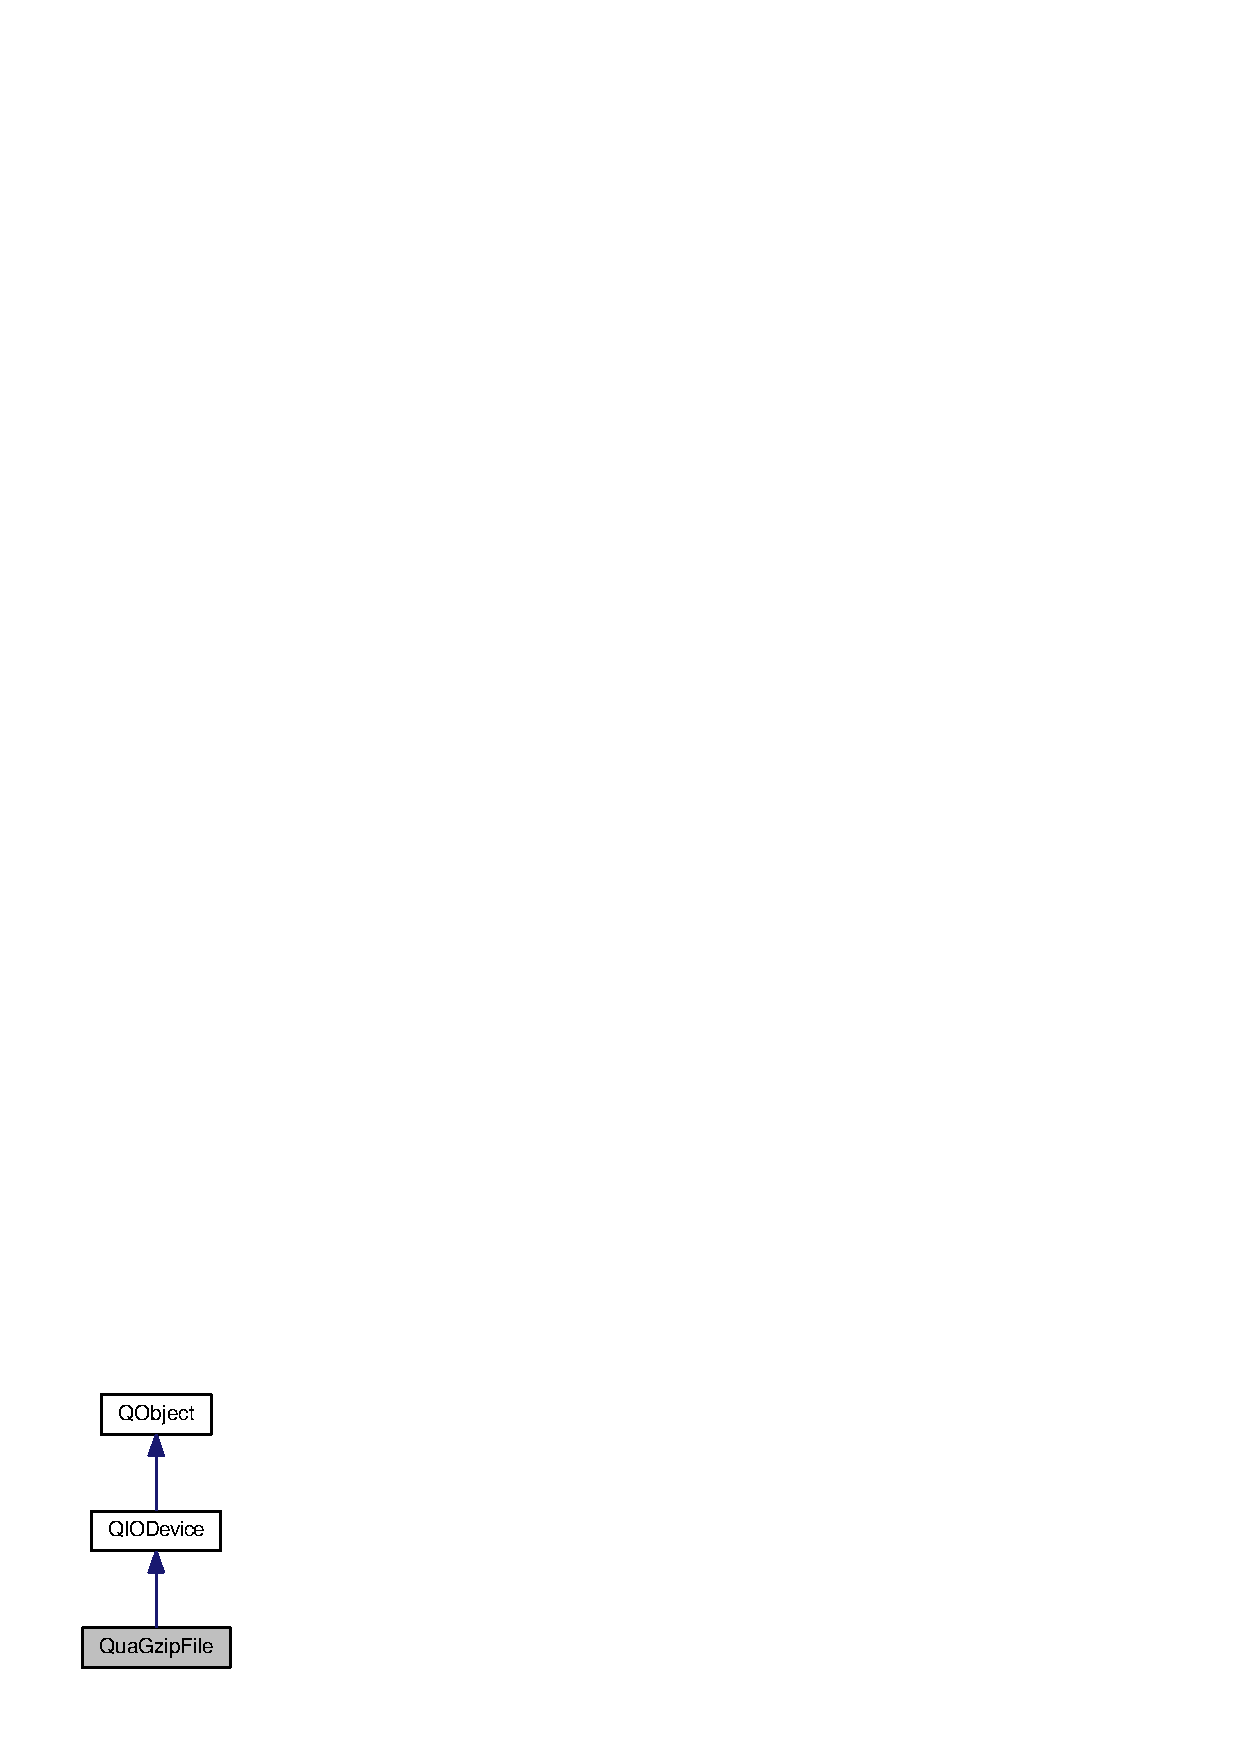
\includegraphics[width=114pt]{classQuaGzipFile__coll__graph}
\end{center}
\end{figure}
\subsection*{Public Member Functions}
\begin{DoxyCompactItemize}
\item 
{\bf QuaGzipFile} ()
\begin{DoxyCompactList}\small\item\em Empty constructor. \end{DoxyCompactList}\item 
{\bf QuaGzipFile} ({\bf QObject} $\ast${\bf parent})
\begin{DoxyCompactList}\small\item\em Empty constructor with a parent. \end{DoxyCompactList}\item 
{\bf QuaGzipFile} (const {\bf QString} \&fileName, {\bf QObject} $\ast${\bf parent}=NULL)
\begin{DoxyCompactList}\small\item\em Constructor. \end{DoxyCompactList}\item 
virtual {\bf $\sim$QuaGzipFile} ()\label{classQuaGzipFile_a1200bc76f36bb2e1991e1e0467befbf2}

\begin{DoxyCompactList}\small\item\em Destructor. \end{DoxyCompactList}\item 
void {\bf setFileName} (const {\bf QString} \&fileName)\label{classQuaGzipFile_a253fbaf410a3d4ae0a719505c5525149}

\begin{DoxyCompactList}\small\item\em Sets the name of the GZIP file to be opened. \end{DoxyCompactList}\item 
{\bf QString} {\bf getFileName} () const \label{classQuaGzipFile_a9a0954a1db1fcf2aeba0530239bce71c}

\begin{DoxyCompactList}\small\item\em Returns the name of the GZIP file. \end{DoxyCompactList}\item 
virtual bool {\bf isSequential} () const 
\begin{DoxyCompactList}\small\item\em Returns true. \end{DoxyCompactList}\item 
virtual bool {\bf open} ({\bf QIODevice::OpenMode} mode)
\begin{DoxyCompactList}\small\item\em Opens the file. \end{DoxyCompactList}\item 
virtual bool {\bf open} (int fd, {\bf QIODevice::OpenMode} mode)
\begin{DoxyCompactList}\small\item\em Opens the file. \end{DoxyCompactList}\item 
virtual bool {\bf flush} ()
\begin{DoxyCompactList}\small\item\em Flushes data to file. \end{DoxyCompactList}\item 
virtual void {\bf close} ()\label{classQuaGzipFile_a273205350b1235a242a1eb5cbf586434}

\begin{DoxyCompactList}\small\item\em Closes the file. \end{DoxyCompactList}\end{DoxyCompactItemize}
\subsection*{Protected Member Functions}
\begin{DoxyCompactItemize}
\item 
virtual qint64 {\bf readData} (char $\ast$data, qint64 maxSize)\label{classQuaGzipFile_a9eab41b46367e63e0c269c42ca883d82}

\begin{DoxyCompactList}\small\item\em Implementation of {\bf QIODevice::readData()}. \end{DoxyCompactList}\item 
virtual qint64 {\bf writeData} (const char $\ast$data, qint64 maxSize)\label{classQuaGzipFile_a6dd09d41d8a51c96b0f2134eff37f676}

\begin{DoxyCompactList}\small\item\em Implementation of {\bf QIODevice::writeData()}. \end{DoxyCompactList}\end{DoxyCompactItemize}


\subsection{Detailed Description}
GZIP file. 

This class is a wrapper around GZIP file access functions in zlib. Unlike \doxyref{QuaZip}{p.}{classQuaZip} classes, it doesn't allow reading from a GZIP file opened as {\bf QIODevice}, for example, if your GZIP file is in {\bf QBuffer}. It only provides {\bf QIODevice} access to a GZIP file contents, but the GZIP file itself must be identified by its name on disk or by descriptor id. 

\subsection{Constructor \& Destructor Documentation}
\index{QuaGzipFile@{QuaGzipFile}!QuaGzipFile@{QuaGzipFile}}
\index{QuaGzipFile@{QuaGzipFile}!QuaGzipFile@{QuaGzipFile}}
\subsubsection[{QuaGzipFile}]{\setlength{\rightskip}{0pt plus 5cm}QuaGzipFile::QuaGzipFile (
\begin{DoxyParamCaption}
{}
\end{DoxyParamCaption}
)}\label{classQuaGzipFile_a709608207b41ca81d5beed2b34982809}


Empty constructor. 

Must call \doxyref{setFileName()}{p.}{classQuaGzipFile_a253fbaf410a3d4ae0a719505c5525149} before trying to open. \index{QuaGzipFile@{QuaGzipFile}!QuaGzipFile@{QuaGzipFile}}
\index{QuaGzipFile@{QuaGzipFile}!QuaGzipFile@{QuaGzipFile}}
\subsubsection[{QuaGzipFile}]{\setlength{\rightskip}{0pt plus 5cm}QuaGzipFile::QuaGzipFile (
\begin{DoxyParamCaption}
\item[{{\bf QObject} $\ast$}]{parent}
\end{DoxyParamCaption}
)}\label{classQuaGzipFile_a13996f5db660c4a29645f8d208b9ca6b}


Empty constructor with a parent. 

Must call \doxyref{setFileName()}{p.}{classQuaGzipFile_a253fbaf410a3d4ae0a719505c5525149} before trying to open. 
\begin{DoxyParams}{Parameters}
{\em parent} & The parent object, as per {\bf QObject} logic. \\
\hline
\end{DoxyParams}
\index{QuaGzipFile@{QuaGzipFile}!QuaGzipFile@{QuaGzipFile}}
\index{QuaGzipFile@{QuaGzipFile}!QuaGzipFile@{QuaGzipFile}}
\subsubsection[{QuaGzipFile}]{\setlength{\rightskip}{0pt plus 5cm}QuaGzipFile::QuaGzipFile (
\begin{DoxyParamCaption}
\item[{const {\bf QString} \&}]{fileName, }
\item[{{\bf QObject} $\ast$}]{parent = {\ttfamily NULL}}
\end{DoxyParamCaption}
)}\label{classQuaGzipFile_ac7f7703bda9c6169c001aa15641bb2ea}


Constructor. 


\begin{DoxyParams}{Parameters}
{\em fileName} & The name of the GZIP file. \\
\hline
{\em parent} & The parent object, as per {\bf QObject} logic. \\
\hline
\end{DoxyParams}


\subsection{Member Function Documentation}
\index{QuaGzipFile@{QuaGzipFile}!isSequential@{isSequential}}
\index{isSequential@{isSequential}!QuaGzipFile@{QuaGzipFile}}
\subsubsection[{isSequential}]{\setlength{\rightskip}{0pt plus 5cm}bool QuaGzipFile::isSequential (
\begin{DoxyParamCaption}
{}
\end{DoxyParamCaption}
) const\hspace{0.3cm}{\ttfamily  [virtual]}}\label{classQuaGzipFile_ae97f4e15d86c965c156df33d00318176}


Returns true. 

Strictly speaking, zlib supports seeking for GZIP files, but it is poorly implemented, because there is no way to implement it properly. For reading, seeking backwards is very slow, and for writing, it is downright impossible. Therefore, \doxyref{QuaGzipFile}{p.}{classQuaGzipFile} does not support seeking at all. 

Reimplemented from {\bf QIODevice}.

\index{QuaGzipFile@{QuaGzipFile}!open@{open}}
\index{open@{open}!QuaGzipFile@{QuaGzipFile}}
\subsubsection[{open}]{\setlength{\rightskip}{0pt plus 5cm}bool QuaGzipFile::open (
\begin{DoxyParamCaption}
\item[{{\bf QIODevice::OpenMode}}]{mode}
\end{DoxyParamCaption}
)\hspace{0.3cm}{\ttfamily  [virtual]}}\label{classQuaGzipFile_a1d560babdfff3a3441d704099a5bc1e4}


Opens the file. 


\begin{DoxyParams}{Parameters}
{\em mode} & Can be either QIODevice::Write or QIODevice::Read. ReadWrite and Append aren't supported. \\
\hline
\end{DoxyParams}


References QIODevice::setErrorString().



Referenced by open().

\index{QuaGzipFile@{QuaGzipFile}!open@{open}}
\index{open@{open}!QuaGzipFile@{QuaGzipFile}}
\subsubsection[{open}]{\setlength{\rightskip}{0pt plus 5cm}bool QuaGzipFile::open (
\begin{DoxyParamCaption}
\item[{int}]{fd, }
\item[{{\bf QIODevice::OpenMode}}]{mode}
\end{DoxyParamCaption}
)\hspace{0.3cm}{\ttfamily  [virtual]}}\label{classQuaGzipFile_adf5a954bb9bfda2d33cd336a213e2549}


Opens the file. 

This is an overloaded member function, provided for convenience. It differs from the above function only in what argument(s) it accepts. 
\begin{DoxyParams}{Parameters}
{\em fd} & The file descriptor to read/write the GZIP file from/to. \\
\hline
{\em mode} & Can be either QIODevice::Write or QIODevice::Read. ReadWrite and Append aren't supported. \\
\hline
\end{DoxyParams}


References open(), and QIODevice::setErrorString().

\index{QuaGzipFile@{QuaGzipFile}!flush@{flush}}
\index{flush@{flush}!QuaGzipFile@{QuaGzipFile}}
\subsubsection[{flush}]{\setlength{\rightskip}{0pt plus 5cm}bool QuaGzipFile::flush (
\begin{DoxyParamCaption}
{}
\end{DoxyParamCaption}
)\hspace{0.3cm}{\ttfamily  [virtual]}}\label{classQuaGzipFile_ab745f345b727c81abbc3eb5af4dca844}


Flushes data to file. 

The data is written using Z\_\-SYNC\_\-FLUSH mode. Doesn't make any sense when reading. 

The documentation for this class was generated from the following files:\begin{DoxyCompactItemize}
\item 
quazip/quagzipfile.h\item 
quazip/quagzipfile.cpp\end{DoxyCompactItemize}

\section{QuaZIODevice Class Reference}
\label{classQuaZIODevice}\index{QuaZIODevice@{QuaZIODevice}}


A class to compress/decompress {\bf QIODevice}.  




{\ttfamily \#include $<$quaziodevice.h$>$}



Inheritance diagram for QuaZIODevice:
\nopagebreak
\begin{figure}[H]
\begin{center}
\leavevmode
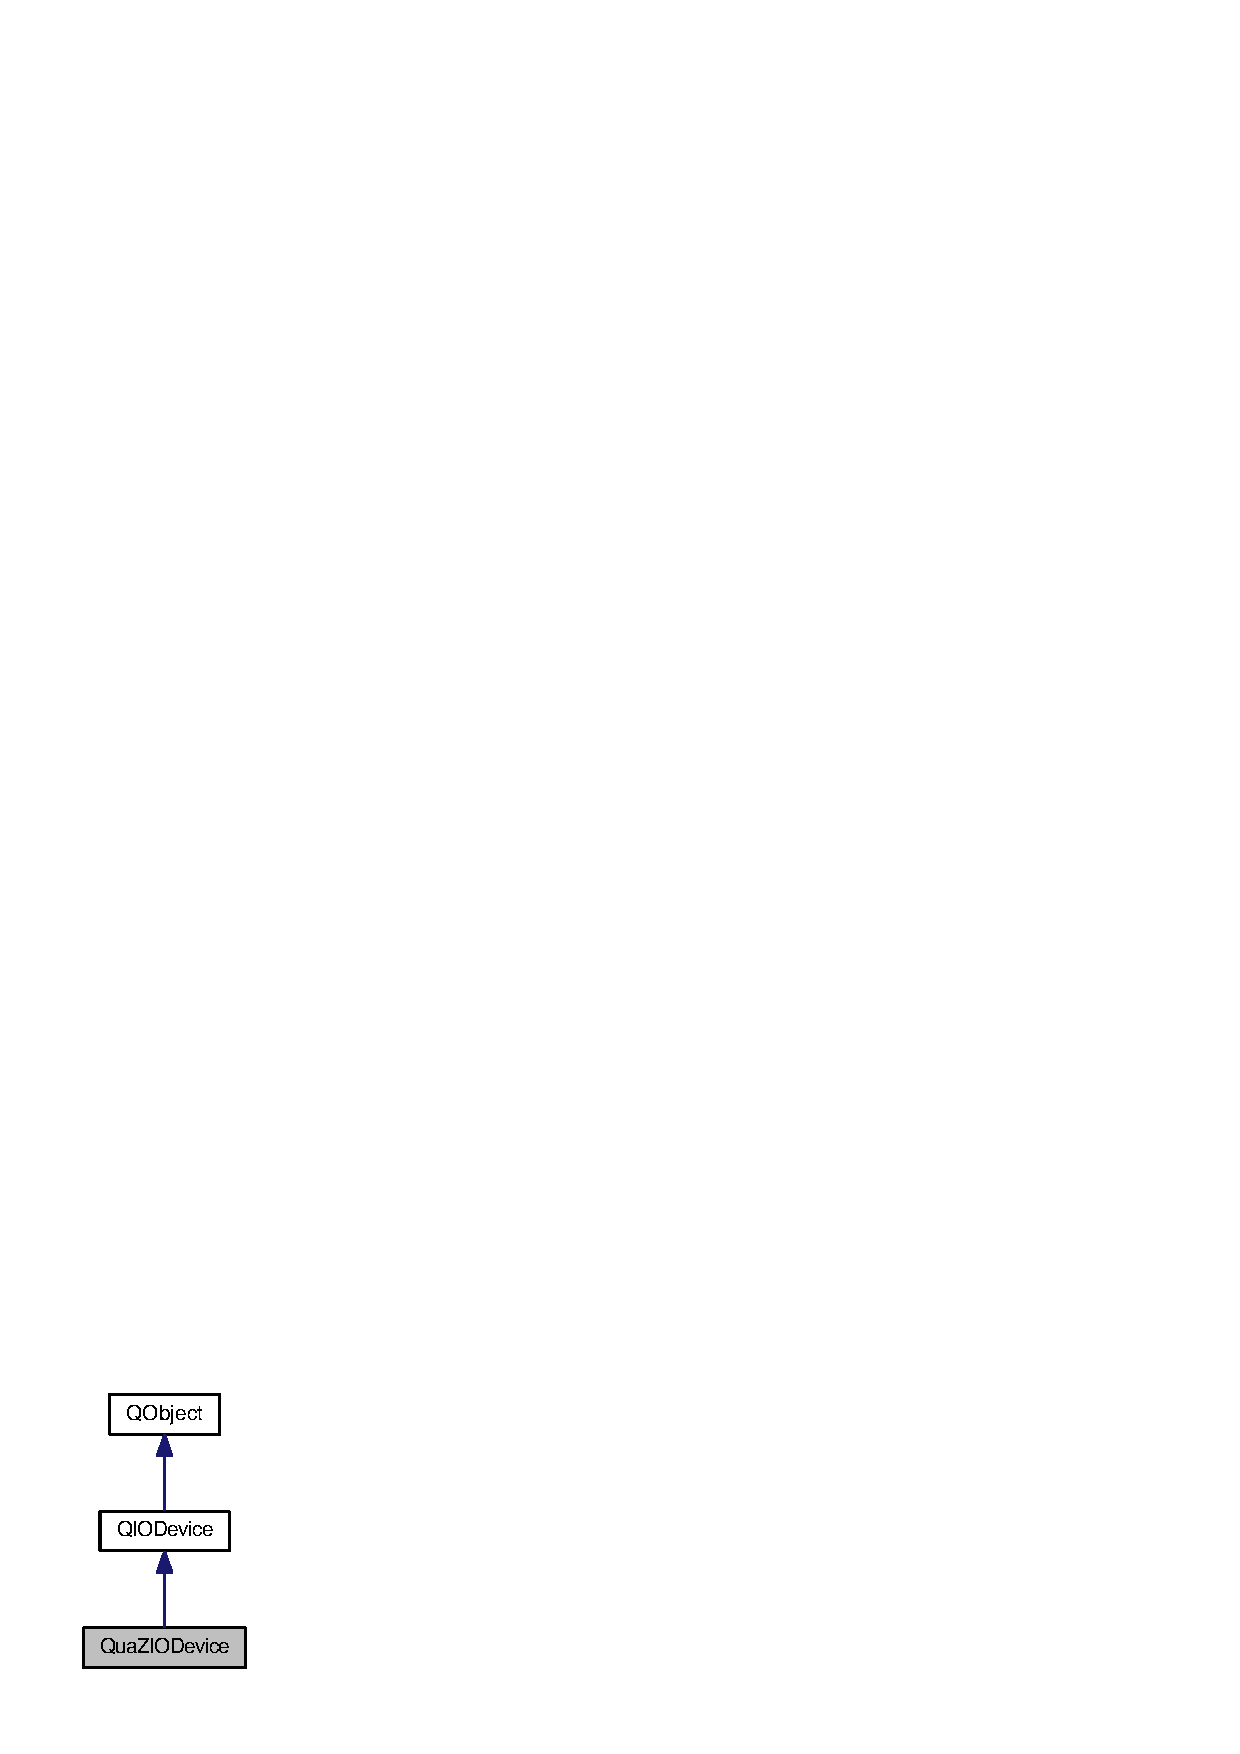
\includegraphics[width=122pt]{classQuaZIODevice__inherit__graph}
\end{center}
\end{figure}


Collaboration diagram for QuaZIODevice:
\nopagebreak
\begin{figure}[H]
\begin{center}
\leavevmode
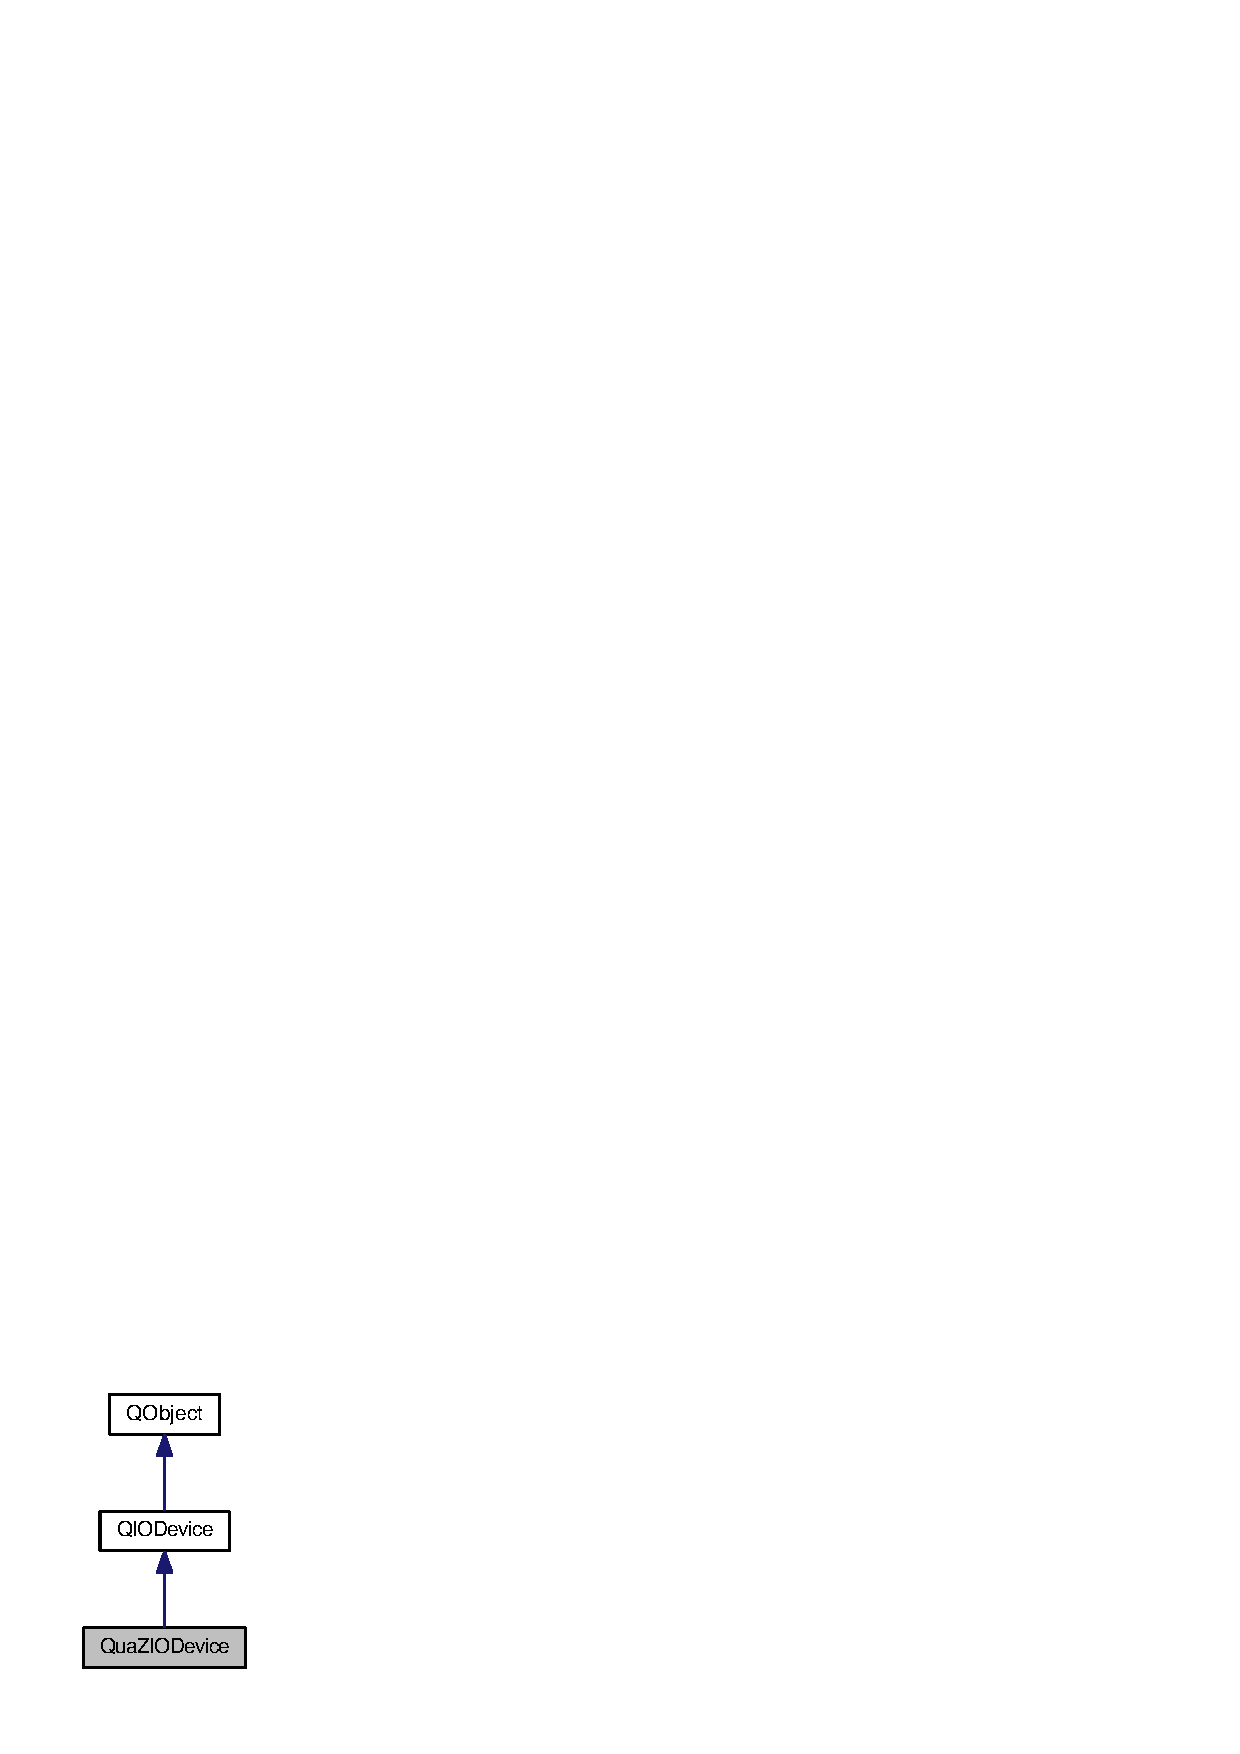
\includegraphics[width=122pt]{classQuaZIODevice__coll__graph}
\end{center}
\end{figure}
\subsection*{Public Member Functions}
\begin{DoxyCompactItemize}
\item 
{\bf QuaZIODevice} ({\bf QIODevice} $\ast$io, {\bf QObject} $\ast${\bf parent}=NULL)
\begin{DoxyCompactList}\small\item\em Constructor. \end{DoxyCompactList}\item 
{\bf $\sim$QuaZIODevice} ()\label{classQuaZIODevice_ab3524cef44c240c21e6b7680ee5f42de}

\begin{DoxyCompactList}\small\item\em Destructor. \end{DoxyCompactList}\item 
virtual bool {\bf flush} ()
\begin{DoxyCompactList}\small\item\em Flushes data waiting to be written. \end{DoxyCompactList}\item 
virtual bool {\bf open} ({\bf QIODevice::OpenMode} mode)
\begin{DoxyCompactList}\small\item\em Opens the device. \end{DoxyCompactList}\item 
virtual void {\bf close} ()
\begin{DoxyCompactList}\small\item\em Closes this device, but not the underlying one. \end{DoxyCompactList}\item 
{\bf QIODevice} $\ast$ {\bf getIoDevice} () const \label{classQuaZIODevice_ad63e7f1717c7d91b3c2c5ace908c98b7}

\begin{DoxyCompactList}\small\item\em Returns the underlying device. \end{DoxyCompactList}\item 
virtual bool {\bf isSequential} () const \label{classQuaZIODevice_af2697f58c228741d3715801bf48a9a8b}

\begin{DoxyCompactList}\small\item\em Returns true. \end{DoxyCompactList}\item 
virtual bool {\bf atEnd} () const \label{classQuaZIODevice_ae727c48089ca1b161323ec8423a653ab}

\begin{DoxyCompactList}\small\item\em Returns true iff the end of the compressed stream is reached. \end{DoxyCompactList}\item 
virtual qint64 {\bf bytesAvailable} () const \label{classQuaZIODevice_ac18b45c3d7009c8d231b13fe994ebcb9}

\begin{DoxyCompactList}\small\item\em Returns the number of the bytes buffered. \end{DoxyCompactList}\end{DoxyCompactItemize}
\subsection*{Protected Member Functions}
\begin{DoxyCompactItemize}
\item 
virtual qint64 {\bf readData} (char $\ast$data, qint64 maxSize)\label{classQuaZIODevice_aa12b8bc9c923e543eda9ae22dbd1ecbb}

\begin{DoxyCompactList}\small\item\em Implementation of {\bf QIODevice::readData()}. \end{DoxyCompactList}\item 
virtual qint64 {\bf writeData} (const char $\ast$data, qint64 maxSize)\label{classQuaZIODevice_aab23b6badbc3548eb71ca86bf6211902}

\begin{DoxyCompactList}\small\item\em Implementation of {\bf QIODevice::writeData()}. \end{DoxyCompactList}\end{DoxyCompactItemize}


\subsection{Detailed Description}
A class to compress/decompress {\bf QIODevice}. 

This class can be used to compress any data written to {\bf QIODevice} or decompress it back. Compressing data sent over a QTcpSocket is a good example. 

\subsection{Constructor \& Destructor Documentation}
\index{QuaZIODevice@{QuaZIODevice}!QuaZIODevice@{QuaZIODevice}}
\index{QuaZIODevice@{QuaZIODevice}!QuaZIODevice@{QuaZIODevice}}
\subsubsection[{QuaZIODevice}]{\setlength{\rightskip}{0pt plus 5cm}QuaZIODevice::QuaZIODevice (
\begin{DoxyParamCaption}
\item[{{\bf QIODevice} $\ast$}]{io, }
\item[{{\bf QObject} $\ast$}]{parent = {\ttfamily NULL}}
\end{DoxyParamCaption}
)}\label{classQuaZIODevice_a8321ed35ee9b57cf9b1104912e236361}


Constructor. 


\begin{DoxyParams}{Parameters}
{\em io} & The {\bf QIODevice} to read/write. \\
\hline
{\em parent} & The parent object, as per {\bf QObject} logic. \\
\hline
\end{DoxyParams}


References QObject::connect(), and QIODevice::readyRead().



\subsection{Member Function Documentation}
\index{QuaZIODevice@{QuaZIODevice}!flush@{flush}}
\index{flush@{flush}!QuaZIODevice@{QuaZIODevice}}
\subsubsection[{flush}]{\setlength{\rightskip}{0pt plus 5cm}bool QuaZIODevice::flush (
\begin{DoxyParamCaption}
{}
\end{DoxyParamCaption}
)\hspace{0.3cm}{\ttfamily  [virtual]}}\label{classQuaZIODevice_a25f586eb564841b51c395fd17f1cc080}


Flushes data waiting to be written. 

Unfortunately, as {\bf QIODevice} doesn't support \doxyref{flush()}{p.}{classQuaZIODevice_a25f586eb564841b51c395fd17f1cc080} by itself, the only thing this method does is write the compressed data into the device using Z\_\-SYNC\_\-FLUSH mode. If you need the compressed data to actually be flushed from the buffer of the underlying {\bf QIODevice}, you need to call its \doxyref{flush()}{p.}{classQuaZIODevice_a25f586eb564841b51c395fd17f1cc080} method as well, providing it supports it (like QTcpSocket does). Example: 
\begin{DoxyCode}
    QuaZIODevice dev(&sock);
    dev.open(QIODevice::Write);
    dev.write(yourDataGoesHere);
    dev.flush();
    sock->flush(); // this actually sends data to network
\end{DoxyCode}


This may change in the future versions of QuaZIP by implementing an ugly hack: trying to cast the {\bf QIODevice} using qobject\_\-cast to known \doxyref{flush()}{p.}{classQuaZIODevice_a25f586eb564841b51c395fd17f1cc080}-\/supporting subclasses, and calling flush if the resulting pointer is not zero. 

References QString::fromLocal8Bit(), and QIODevice::setErrorString().



Referenced by close().

\index{QuaZIODevice@{QuaZIODevice}!open@{open}}
\index{open@{open}!QuaZIODevice@{QuaZIODevice}}
\subsubsection[{open}]{\setlength{\rightskip}{0pt plus 5cm}bool QuaZIODevice::open (
\begin{DoxyParamCaption}
\item[{{\bf QIODevice::OpenMode}}]{mode}
\end{DoxyParamCaption}
)\hspace{0.3cm}{\ttfamily  [virtual]}}\label{classQuaZIODevice_a175446c18eb20c9aff6faf23f09cc67a}


Opens the device. 


\begin{DoxyParams}{Parameters}
{\em mode} & Neither QIODevice::ReadWrite nor QIODevice::Append are not supported. \\
\hline
\end{DoxyParams}


References QIODevice::setErrorString(), and QObject::trUtf8().

\index{QuaZIODevice@{QuaZIODevice}!close@{close}}
\index{close@{close}!QuaZIODevice@{QuaZIODevice}}
\subsubsection[{close}]{\setlength{\rightskip}{0pt plus 5cm}void QuaZIODevice::close (
\begin{DoxyParamCaption}
{}
\end{DoxyParamCaption}
)\hspace{0.3cm}{\ttfamily  [virtual]}}\label{classQuaZIODevice_ad27e447544d57f897316ee6f44535895}


Closes this device, but not the underlying one. 

The underlying {\bf QIODevice} is not closed in case you want to write something else to it. 

Reimplemented from {\bf QIODevice}.



References flush(), QIODevice::openMode(), and QIODevice::setErrorString().



Referenced by $\sim$QuaZIODevice().



The documentation for this class was generated from the following files:\begin{DoxyCompactItemize}
\item 
quazip/quaziodevice.h\item 
quazip/quaziodevice.cpp\end{DoxyCompactItemize}

\section{QuaZip Class Reference}
\label{classQuaZip}\index{QuaZip@{QuaZip}}


ZIP archive.  




{\ttfamily \#include $<$quazip/quazip.h$>$}



Collaboration diagram for QuaZip:
\nopagebreak
\begin{figure}[H]
\begin{center}
\leavevmode
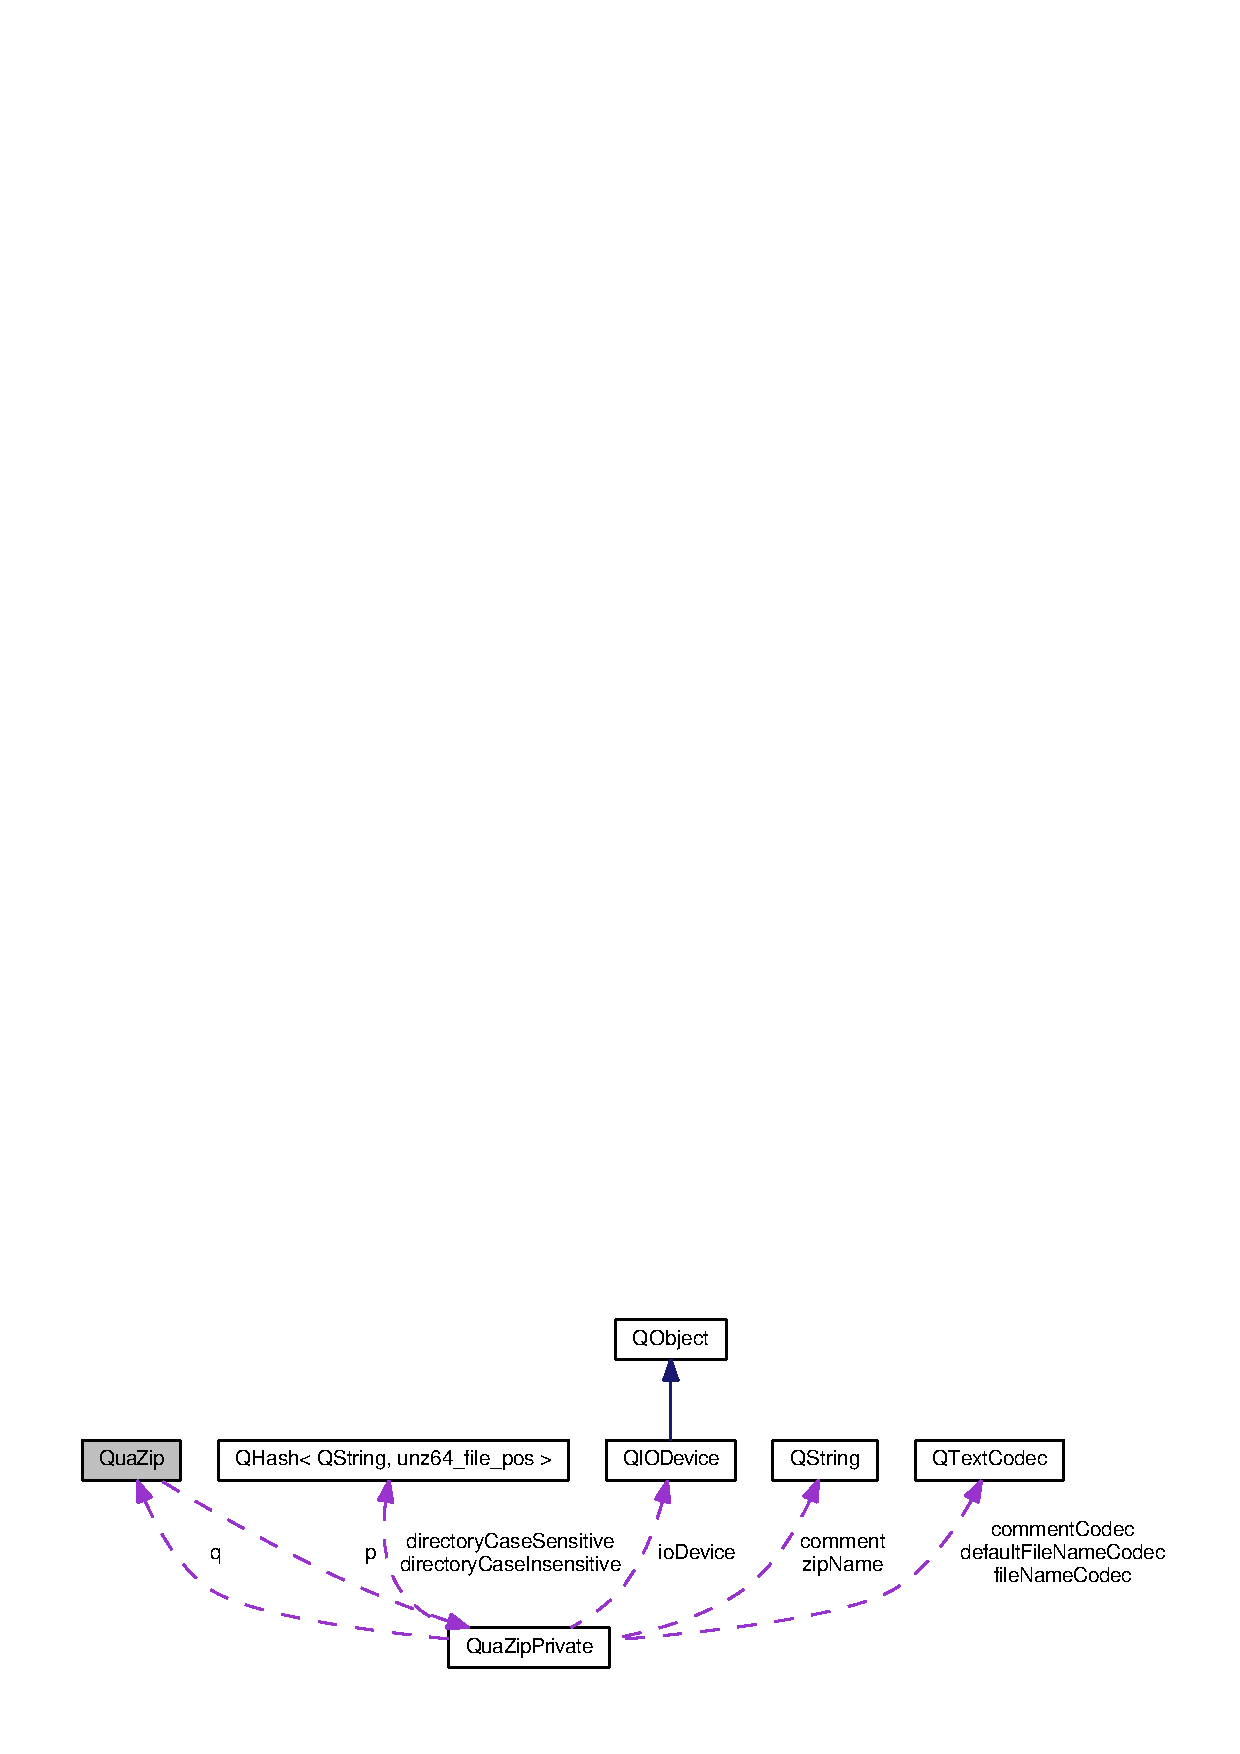
\includegraphics[width=400pt]{classQuaZip__coll__graph}
\end{center}
\end{figure}
\subsection*{Public Types}
\begin{DoxyCompactItemize}
\item 
enum {\bf Constants} \{ {\bf MAX\_\-FILE\_\-NAME\_\-LENGTH} = 256
 \}
\begin{DoxyCompactList}\small\item\em Useful constants. \end{DoxyCompactList}\item 
enum {\bf Mode} \{ \par
{\bf mdNotOpen}, 
{\bf mdUnzip}, 
{\bf mdCreate}, 
{\bf mdAppend}, 
\par
{\bf mdAdd}
 \}
\begin{DoxyCompactList}\small\item\em Open mode of the ZIP file. \end{DoxyCompactList}\item 
enum {\bf CaseSensitivity} \{ {\bf csDefault} = 0, 
{\bf csSensitive} = 1, 
{\bf csInsensitive} = 2
 \}
\begin{DoxyCompactList}\small\item\em Case sensitivity for the file names. \end{DoxyCompactList}\end{DoxyCompactItemize}
\subsection*{Public Member Functions}
\begin{DoxyCompactItemize}
\item 
{\bf QuaZip} ()
\begin{DoxyCompactList}\small\item\em Constructs \doxyref{QuaZip}{p.}{classQuaZip} object. \end{DoxyCompactList}\item 
{\bf QuaZip} (const {\bf QString} \&zipName)\label{classQuaZip_aaea7294b02abd22379cc3a9fccb754b7}

\begin{DoxyCompactList}\small\item\em Constructs \doxyref{QuaZip}{p.}{classQuaZip} object associated with ZIP file {\itshape zipName\/}. \end{DoxyCompactList}\item 
{\bf QuaZip} ({\bf QIODevice} $\ast$ioDevice)
\begin{DoxyCompactList}\small\item\em Constructs \doxyref{QuaZip}{p.}{classQuaZip} object associated with ZIP file represented by {\itshape ioDevice\/}. \end{DoxyCompactList}\item 
{\bf $\sim$QuaZip} ()
\begin{DoxyCompactList}\small\item\em Destroys \doxyref{QuaZip}{p.}{classQuaZip} object. \end{DoxyCompactList}\item 
bool {\bf open} ({\bf Mode} mode, zlib\_\-filefunc\_\-def $\ast$ioApi=NULL)
\begin{DoxyCompactList}\small\item\em Opens ZIP file. \end{DoxyCompactList}\item 
void {\bf close} ()
\begin{DoxyCompactList}\small\item\em Closes ZIP file. \end{DoxyCompactList}\item 
void {\bf setFileNameCodec} ({\bf QTextCodec} $\ast$fileNameCodec)
\begin{DoxyCompactList}\small\item\em Sets the codec used to encode/decode file names inside archive. \end{DoxyCompactList}\item 
void {\bf setFileNameCodec} (const char $\ast$fileNameCodecName)
\begin{DoxyCompactList}\small\item\em Sets the codec used to encode/decode file names inside archive. \end{DoxyCompactList}\item 
{\bf QTextCodec} $\ast$ {\bf getFileNameCodec} () const \label{classQuaZip_a27b866aa2c75ea6f9c438cbb6e32b43c}

\begin{DoxyCompactList}\small\item\em Returns the codec used to encode/decode comments inside archive. \end{DoxyCompactList}\item 
void {\bf setCommentCodec} ({\bf QTextCodec} $\ast$commentCodec)
\begin{DoxyCompactList}\small\item\em Sets the codec used to encode/decode comments inside archive. \end{DoxyCompactList}\item 
void {\bf setCommentCodec} (const char $\ast$commentCodecName)
\begin{DoxyCompactList}\small\item\em Sets the codec used to encode/decode comments inside archive. \end{DoxyCompactList}\item 
{\bf QTextCodec} $\ast$ {\bf getCommentCodec} () const \label{classQuaZip_a008260161781d8b5d2a0a28493fddaf4}

\begin{DoxyCompactList}\small\item\em Returns the codec used to encode/decode comments inside archive. \end{DoxyCompactList}\item 
{\bf QString} {\bf getZipName} () const 
\begin{DoxyCompactList}\small\item\em Returns the name of the ZIP file. \end{DoxyCompactList}\item 
void {\bf setZipName} (const {\bf QString} \&zipName)
\begin{DoxyCompactList}\small\item\em Sets the name of the ZIP file. \end{DoxyCompactList}\item 
{\bf QIODevice} $\ast$ {\bf getIoDevice} () const 
\begin{DoxyCompactList}\small\item\em Returns the device representing this ZIP file. \end{DoxyCompactList}\item 
void {\bf setIoDevice} ({\bf QIODevice} $\ast$ioDevice)
\begin{DoxyCompactList}\small\item\em Sets the device representing the ZIP file. \end{DoxyCompactList}\item 
{\bf Mode} {\bf getMode} () const \label{classQuaZip_a129ceff04d28fb00531f7bf7f9329664}

\begin{DoxyCompactList}\small\item\em Returns the mode in which ZIP file was opened. \end{DoxyCompactList}\item 
bool {\bf isOpen} () const \label{classQuaZip_a5b869a9c0d4f49955b759592fec08888}

\begin{DoxyCompactList}\small\item\em Returns {\ttfamily true} if ZIP file is open, {\ttfamily false} otherwise. \end{DoxyCompactList}\item 
int {\bf getZipError} () const 
\begin{DoxyCompactList}\small\item\em Returns the error code of the last operation. \end{DoxyCompactList}\item 
int {\bf getEntriesCount} () const 
\begin{DoxyCompactList}\small\item\em Returns number of the entries in the ZIP central directory. \end{DoxyCompactList}\item 
{\bf QString} {\bf getComment} () const \label{classQuaZip_ae55cfbf2296132df808c557b62433051}

\begin{DoxyCompactList}\small\item\em Returns global comment in the ZIP file. \end{DoxyCompactList}\item 
void {\bf setComment} (const {\bf QString} \&comment)
\begin{DoxyCompactList}\small\item\em Sets the global comment in the ZIP file. \end{DoxyCompactList}\item 
bool {\bf goToFirstFile} ()
\begin{DoxyCompactList}\small\item\em Sets the current file to the first file in the archive. \end{DoxyCompactList}\item 
bool {\bf goToNextFile} ()
\begin{DoxyCompactList}\small\item\em Sets the current file to the next file in the archive. \end{DoxyCompactList}\item 
bool {\bf setCurrentFile} (const {\bf QString} \&fileName, {\bf CaseSensitivity} cs=csDefault)
\begin{DoxyCompactList}\small\item\em Sets current file by its name. \end{DoxyCompactList}\item 
bool {\bf hasCurrentFile} () const \label{classQuaZip_a00b237d926648f45da86db25e7cfb697}

\begin{DoxyCompactList}\small\item\em Returns {\ttfamily true} if the current file has been set. \end{DoxyCompactList}\item 
bool {\bf getCurrentFileInfo} ({\bf QuaZipFileInfo} $\ast$info) const 
\begin{DoxyCompactList}\small\item\em Retrieves information about the current file. \end{DoxyCompactList}\item 
bool {\bf getCurrentFileInfo} ({\bf QuaZipFileInfo64} $\ast$info) const 
\begin{DoxyCompactList}\small\item\em Retrieves information about the current file. \end{DoxyCompactList}\item 
{\bf QString} {\bf getCurrentFileName} () const 
\begin{DoxyCompactList}\small\item\em Returns the current file name. \end{DoxyCompactList}\item 
unzFile {\bf getUnzFile} ()
\begin{DoxyCompactList}\small\item\em Returns {\ttfamily unzFile} handle. \end{DoxyCompactList}\item 
zipFile {\bf getZipFile} ()
\begin{DoxyCompactList}\small\item\em Returns {\ttfamily zipFile} handle. \end{DoxyCompactList}\item 
void {\bf setDataDescriptorWritingEnabled} (bool enabled)
\begin{DoxyCompactList}\small\item\em Changes the data descriptor writing mode. \end{DoxyCompactList}\item 
bool {\bf isDataDescriptorWritingEnabled} () const 
\begin{DoxyCompactList}\small\item\em Returns the data descriptor default writing mode. \end{DoxyCompactList}\item 
{\bf QStringList} {\bf getFileNameList} () const 
\begin{DoxyCompactList}\small\item\em Returns a list of files inside the archive. \end{DoxyCompactList}\item 
{\bf QList}$<$ {\bf QuaZipFileInfo} $>$ {\bf getFileInfoList} () const 
\begin{DoxyCompactList}\small\item\em Returns information list about all files inside the archive. \end{DoxyCompactList}\item 
{\bf QList}$<$ {\bf QuaZipFileInfo64} $>$ {\bf getFileInfoList64} () const 
\begin{DoxyCompactList}\small\item\em Returns information list about all files inside the archive. \end{DoxyCompactList}\item 
void {\bf setZip64Enabled} (bool zip64)
\begin{DoxyCompactList}\small\item\em Enables the zip64 mode. \end{DoxyCompactList}\item 
bool {\bf isZip64Enabled} () const 
\begin{DoxyCompactList}\small\item\em Returns whether the zip64 mode is enabled. \end{DoxyCompactList}\item 
bool {\bf isAutoClose} () const 
\begin{DoxyCompactList}\small\item\em Returns the auto-\/close flag. \end{DoxyCompactList}\item 
void {\bf setAutoClose} (bool autoClose) const 
\begin{DoxyCompactList}\small\item\em Sets or unsets the auto-\/close flag. \end{DoxyCompactList}\end{DoxyCompactItemize}
\subsection*{Static Public Member Functions}
\begin{DoxyCompactItemize}
\item 
static Qt::CaseSensitivity {\bf convertCaseSensitivity} ({\bf CaseSensitivity} cs)
\begin{DoxyCompactList}\small\item\em Returns the actual case sensitivity for the specified QuaZIP one. \end{DoxyCompactList}\item 
static void {\bf setDefaultFileNameCodec} ({\bf QTextCodec} $\ast$codec)
\begin{DoxyCompactList}\small\item\em Sets the default file name codec to use. \end{DoxyCompactList}\item 
static void {\bf setDefaultFileNameCodec} (const char $\ast$codecName)
\end{DoxyCompactItemize}
\subsection*{Friends}
\begin{DoxyCompactItemize}
\item 
class {\bf QuaZipPrivate}\label{classQuaZip_a5d400b33a69412e9d419a484aaf476cd}

\end{DoxyCompactItemize}


\subsection{Detailed Description}
ZIP archive. 

This class implements basic interface to the ZIP archive. It can be used to read table contents of the ZIP archive and retreiving information about the files inside it.

You can also use this class to open files inside archive by passing pointer to the instance of this class to the constructor of the \doxyref{QuaZipFile}{p.}{classQuaZipFile} class. But see \doxyref{QuaZipFile::QuaZipFile(QuaZip$\ast$, QObject$\ast$)}{p.}{classQuaZipFile_a54e944a6b3d27030f64c8f30d2cc33bb} for the possible pitfalls.

This class is indended to provide interface to the ZIP subpackage of the ZIP/UNZIP package as well as to the UNZIP subpackage. But currently it supports only UNZIP.

The use of this class is simple -\/ just create instance using constructor, then set ZIP archive file name using setFile() function (if you did not passed the name to the constructor), then \doxyref{open()}{p.}{classQuaZip_abfa4e6018b2964a3d10a4c54e5ab3962} and then use different functions to work with it! Well, if you are paranoid, you may also wish to call close before destructing the instance, to check for errors on close.

You may also use \doxyref{getUnzFile()}{p.}{classQuaZip_a3b78a652f296ff4a678a791e8294e642} and \doxyref{getZipFile()}{p.}{classQuaZip_a425043a4d7cc31e2fe2bba73d954f15c} functions to get the ZIP archive handle and use it with ZIP/UNZIP package API directly.

This class supports localized file names inside ZIP archive, but you have to set up proper codec with setCodec() function. By default, locale codec will be used, which is probably ok for UNIX systems, but will almost certainly fail with ZIP archives created in Windows. This is because Windows ZIP programs have strange habit of using DOS encoding for file names in ZIP archives. For example, ZIP archive with cyrillic names created in Windows will have file names in {\ttfamily IBM866} encoding instead of {\ttfamily WINDOWS-\/1251}. I think that calling one function is not much trouble, but for true platform independency it would be nice to have some mechanism for file name encoding auto detection using locale information. Does anyone know a good way to do it? 

\subsection{Member Enumeration Documentation}
\index{QuaZip@{QuaZip}!Constants@{Constants}}
\index{Constants@{Constants}!QuaZip@{QuaZip}}
\subsubsection[{Constants}]{\setlength{\rightskip}{0pt plus 5cm}enum {\bf QuaZip::Constants}}\label{classQuaZip_adce46b942c341dbb5c851eadead65459}


Useful constants. 

\begin{Desc}
\item[Enumerator: ]\par
\begin{description}
\index{MAX\_\-FILE\_\-NAME\_\-LENGTH@{MAX\_\-FILE\_\-NAME\_\-LENGTH}!QuaZip@{QuaZip}}\index{QuaZip@{QuaZip}!MAX\_\-FILE\_\-NAME\_\-LENGTH@{MAX\_\-FILE\_\-NAME\_\-LENGTH}}\item[{\em 
MAX\_\-FILE\_\-NAME\_\-LENGTH\label{classQuaZip_adce46b942c341dbb5c851eadead65459ab26ce1a9c9e94f901dc2cf90fa5baa4b}
}]Maximum file name length. Taken from {\ttfamily UNZ\_\-MAXFILENAMEINZIP} constant in unzip.c. \end{description}
\end{Desc}

\index{QuaZip@{QuaZip}!Mode@{Mode}}
\index{Mode@{Mode}!QuaZip@{QuaZip}}
\subsubsection[{Mode}]{\setlength{\rightskip}{0pt plus 5cm}enum {\bf QuaZip::Mode}}\label{classQuaZip_a47e28d4116ee716fdd6b431b821d0be4}


Open mode of the ZIP file. 

\begin{Desc}
\item[Enumerator: ]\par
\begin{description}
\index{mdNotOpen@{mdNotOpen}!QuaZip@{QuaZip}}\index{QuaZip@{QuaZip}!mdNotOpen@{mdNotOpen}}\item[{\em 
mdNotOpen\label{classQuaZip_a47e28d4116ee716fdd6b431b821d0be4ac87ddb1e901e1ec700c16ee0d4d398ce}
}]ZIP file is not open. This is the initial mode. \index{mdUnzip@{mdUnzip}!QuaZip@{QuaZip}}\index{QuaZip@{QuaZip}!mdUnzip@{mdUnzip}}\item[{\em 
mdUnzip\label{classQuaZip_a47e28d4116ee716fdd6b431b821d0be4a803a371910c2dc830d111e9ce5b58897}
}]ZIP file is open for reading files inside it. \index{mdCreate@{mdCreate}!QuaZip@{QuaZip}}\index{QuaZip@{QuaZip}!mdCreate@{mdCreate}}\item[{\em 
mdCreate\label{classQuaZip_a47e28d4116ee716fdd6b431b821d0be4a25ae05b12590540af8c66ae8298b928e}
}]ZIP file was created with \doxyref{open()}{p.}{classQuaZip_abfa4e6018b2964a3d10a4c54e5ab3962} call. \index{mdAppend@{mdAppend}!QuaZip@{QuaZip}}\index{QuaZip@{QuaZip}!mdAppend@{mdAppend}}\item[{\em 
mdAppend\label{classQuaZip_a47e28d4116ee716fdd6b431b821d0be4ab807f0c65653a16d77b365801fd25582}
}]ZIP file was opened in append mode. This refers to {\ttfamily APPEND\_\-STATUS\_\-CREATEAFTER} mode in ZIP/UNZIP package and means that zip is appended to some existing file what is useful when that file contains self-\/extractor code. This is obviously {\itshape not\/} what you whant to use to add files to the existing ZIP archive. \index{mdAdd@{mdAdd}!QuaZip@{QuaZip}}\index{QuaZip@{QuaZip}!mdAdd@{mdAdd}}\item[{\em 
mdAdd\label{classQuaZip_a47e28d4116ee716fdd6b431b821d0be4a22c745f349f06add449af523254fdaec}
}]ZIP file was opened for adding files in the archive. \end{description}
\end{Desc}

\index{QuaZip@{QuaZip}!CaseSensitivity@{CaseSensitivity}}
\index{CaseSensitivity@{CaseSensitivity}!QuaZip@{QuaZip}}
\subsubsection[{CaseSensitivity}]{\setlength{\rightskip}{0pt plus 5cm}enum {\bf QuaZip::CaseSensitivity}}\label{classQuaZip_a6053a1d249ed210a85c9d5eb7cf9cdbe}


Case sensitivity for the file names. 

This is what you specify when accessing files in the archive. Works perfectly fine with any characters thanks to Qt's great unicode support. This is different from ZIP/UNZIP API, where only US-\/ASCII characters was supported. \begin{Desc}
\item[Enumerator: ]\par
\begin{description}
\index{csDefault@{csDefault}!QuaZip@{QuaZip}}\index{QuaZip@{QuaZip}!csDefault@{csDefault}}\item[{\em 
csDefault\label{classQuaZip_a6053a1d249ed210a85c9d5eb7cf9cdbeac3cca8c0b976cf6397a28a5c84e75253}
}]Default for platform. Case sensitive for UNIX, not for Windows. \index{csSensitive@{csSensitive}!QuaZip@{QuaZip}}\index{QuaZip@{QuaZip}!csSensitive@{csSensitive}}\item[{\em 
csSensitive\label{classQuaZip_a6053a1d249ed210a85c9d5eb7cf9cdbead8d86b0c34203336cad09348cfa5356e}
}]Case sensitive. \index{csInsensitive@{csInsensitive}!QuaZip@{QuaZip}}\index{QuaZip@{QuaZip}!csInsensitive@{csInsensitive}}\item[{\em 
csInsensitive\label{classQuaZip_a6053a1d249ed210a85c9d5eb7cf9cdbea3e492bcc3f64f41a74906cecc45fb366}
}]Case insensitive. \end{description}
\end{Desc}



\subsection{Constructor \& Destructor Documentation}
\index{QuaZip@{QuaZip}!QuaZip@{QuaZip}}
\index{QuaZip@{QuaZip}!QuaZip@{QuaZip}}
\subsubsection[{QuaZip}]{\setlength{\rightskip}{0pt plus 5cm}QuaZip::QuaZip (
\begin{DoxyParamCaption}
{}
\end{DoxyParamCaption}
)}\label{classQuaZip_a970e0f401c7cfd7a78e78572f758eec4}


Constructs \doxyref{QuaZip}{p.}{classQuaZip} object. 

Call setName() before opening constructed object. \index{QuaZip@{QuaZip}!QuaZip@{QuaZip}}
\index{QuaZip@{QuaZip}!QuaZip@{QuaZip}}
\subsubsection[{QuaZip}]{\setlength{\rightskip}{0pt plus 5cm}QuaZip::QuaZip (
\begin{DoxyParamCaption}
\item[{{\bf QIODevice} $\ast$}]{ioDevice}
\end{DoxyParamCaption}
)}\label{classQuaZip_ae52ebadd5ce64cdb49d7e198904b0b8c}


Constructs \doxyref{QuaZip}{p.}{classQuaZip} object associated with ZIP file represented by {\itshape ioDevice\/}. 

The IO device must be seekable, otherwise an error will occur when opening. \index{QuaZip@{QuaZip}!$\sim$QuaZip@{$\sim$QuaZip}}
\index{$\sim$QuaZip@{$\sim$QuaZip}!QuaZip@{QuaZip}}
\subsubsection[{$\sim$QuaZip}]{\setlength{\rightskip}{0pt plus 5cm}QuaZip::$\sim$QuaZip (
\begin{DoxyParamCaption}
{}
\end{DoxyParamCaption}
)}\label{classQuaZip_af60a2d3930b90f3b25a3148baecad81e}


Destroys \doxyref{QuaZip}{p.}{classQuaZip} object. 

Calls \doxyref{close()}{p.}{classQuaZip_a7a4323b73e12f3b4470109f200728f9f} if necessary. 

References close(), and isOpen().



\subsection{Member Function Documentation}
\index{QuaZip@{QuaZip}!convertCaseSensitivity@{convertCaseSensitivity}}
\index{convertCaseSensitivity@{convertCaseSensitivity}!QuaZip@{QuaZip}}
\subsubsection[{convertCaseSensitivity}]{\setlength{\rightskip}{0pt plus 5cm}Qt::CaseSensitivity QuaZip::convertCaseSensitivity (
\begin{DoxyParamCaption}
\item[{{\bf QuaZip::CaseSensitivity}}]{cs}
\end{DoxyParamCaption}
)\hspace{0.3cm}{\ttfamily  [static]}}\label{classQuaZip_a1d3fbd445a8e9d3449ded7371931c6b3}


Returns the actual case sensitivity for the specified QuaZIP one. 


\begin{DoxyParams}{Parameters}
{\em cs} & The value to convert. \\
\hline
\end{DoxyParams}
\begin{DoxyReturn}{Returns}
If CaseSensitivity::csDefault, then returns the default file name case sensitivity for the platform. Otherwise, just returns the appropriate value from the Qt::CaseSensitivity enum. 
\end{DoxyReturn}


References csDefault, and csSensitive.



Referenced by QuaZipDir::exists(), and setCurrentFile().

\index{QuaZip@{QuaZip}!open@{open}}
\index{open@{open}!QuaZip@{QuaZip}}
\subsubsection[{open}]{\setlength{\rightskip}{0pt plus 5cm}bool QuaZip::open (
\begin{DoxyParamCaption}
\item[{{\bf Mode}}]{mode, }
\item[{zlib\_\-filefunc\_\-def $\ast$}]{ioApi = {\ttfamily NULL}}
\end{DoxyParamCaption}
)}\label{classQuaZip_abfa4e6018b2964a3d10a4c54e5ab3962}


Opens ZIP file. 

Argument {\itshape mode\/} specifies open mode of the ZIP archive. See Mode for details. Note that there is zipOpen2() function in the ZIP/UNZIP API which accepts {\itshape globalcomment\/} argument, but it does not use it anywhere, so this \doxyref{open()}{p.}{classQuaZip_abfa4e6018b2964a3d10a4c54e5ab3962} function does not have this argument. See \doxyref{setComment()}{p.}{classQuaZip_a1b5d936a203859340574d5908ffa2222} if you need to set global comment.

If the ZIP file is accessed via explicitly set {\bf QIODevice}, then this device is opened in the necessary mode. If the device was already opened by some other means, then QuaZIP checks if the open mode is compatible to the mode needed for the requested operation. If necessary, seeking is performed to position the device properly.

\begin{DoxyReturn}{Returns}
{\ttfamily true} if successful, {\ttfamily false} otherwise.
\end{DoxyReturn}
\begin{DoxyNote}{Note}
ZIP/UNZIP API open calls do not return error code -\/ they just return {\ttfamily NULL} indicating an error. But to make things easier, \doxyref{quazip.h}{p.}{quazip_8h_source} header defines additional error code {\ttfamily UNZ\_\-ERROROPEN} and \doxyref{getZipError()}{p.}{classQuaZip_a28b91a6282ddd9382c96a069572c6fb4} will return it if the open call of the ZIP/UNZIP API returns {\ttfamily NULL}.
\end{DoxyNote}
Argument {\itshape ioApi\/} specifies IO function set for ZIP/UNZIP package to use. See unzip.h, zip.h and ioapi.h for details. Note that IO API for \doxyref{QuaZip}{p.}{classQuaZip} is different from the original package. The file path argument was changed to be of type {\ttfamily voidpf}, and \doxyref{QuaZip}{p.}{classQuaZip} passes a {\bf QIODevice} pointer there. This {\bf QIODevice} is either set explicitly via \doxyref{setIoDevice()}{p.}{classQuaZip_a64642948b6531ee54f5522f29e388cc6} or the \doxyref{QuaZip(QIODevice$\ast$)}{p.}{classQuaZip_ae52ebadd5ce64cdb49d7e198904b0b8c} constructor, or it is created internally when opening the archive by its file name. The default API (qioapi.cpp) just delegates everything to the {\bf QIODevice} API. Not only this allows to use a {\bf QIODevice} instead of file name, but also has a nice side effect of raising the file size limit from 2G to 4G (in non-\/zip64 archives).

\begin{DoxyNote}{Note}
If the zip64 support is needed, the ioApi argument {\itshape must\/} be NULL because due to the backwards compatibility issues it can be used to provide a 32-\/bit API only.

If the \doxyref{no-\/auto-\/close}{p.}{classQuaZip_a54bfc924762774ccf9f99be075ba7b0e} feature is used, then the {\itshape ioApi\/} argument {\itshape should\/} be NULL because the old API doesn't support the 'fake close' operation, causing slight memory leaks and other possible troubles (like closing the output device in case when an error occurs during opening).
\end{DoxyNote}
In short: just forget about the {\itshape ioApi\/} argument and you'll be fine. 

References QString::isEmpty(), isOpen(), QIODevice::isSequential(), mdAdd, mdAppend, mdCreate, mdUnzip, QuaZipPrivate::unzFile\_\-f, and QuaZipPrivate::zipFile\_\-f.



Referenced by JlCompress::compressDir(), JlCompress::compressFile(), JlCompress::compressFiles(), and QuaZipFile::open().

\index{QuaZip@{QuaZip}!close@{close}}
\index{close@{close}!QuaZip@{QuaZip}}
\subsubsection[{close}]{\setlength{\rightskip}{0pt plus 5cm}void QuaZip::close (
\begin{DoxyParamCaption}
{}
\end{DoxyParamCaption}
)}\label{classQuaZip_a7a4323b73e12f3b4470109f200728f9f}


Closes ZIP file. 

Call \doxyref{getZipError()}{p.}{classQuaZip_a28b91a6282ddd9382c96a069572c6fb4} to determine if the close was successful.

If the file was opened by name, then the underlying {\bf QIODevice} is closed and deleted.

If the underlying {\bf QIODevice} was set explicitly using \doxyref{setIoDevice()}{p.}{classQuaZip_a64642948b6531ee54f5522f29e388cc6} or the appropriate constructor, then it is closed if the auto-\/close flag is set (which it is by default). Call \doxyref{setAutoClose()}{p.}{classQuaZip_a54bfc924762774ccf9f99be075ba7b0e} to clear the auto-\/close flag if this behavior is undesirable.

Since {\bf Qt} 5.1, the {\bf QSaveFile} was introduced. It breaks the {\bf QIODevice} API by making \doxyref{close()}{p.}{classQuaZip_a7a4323b73e12f3b4470109f200728f9f} private and crashing the application if it is called from the base class where it is public. It is an excellent example of poor design that illustrates why you should never ever break an is-\/a relationship between the base class and a subclass. QuaZIP works around this bug by checking if the {\bf QIODevice} is an instance of {\bf QSaveFile}, using qobject\_\-cast$<$$>$, and if it is, calls {\bf QSaveFile::commit()} instead of \doxyref{close()}{p.}{classQuaZip_a7a4323b73e12f3b4470109f200728f9f}. It is a really ugly hack, but at least it makes your programs work instead of crashing. Note that if the auto-\/close flag is cleared, then this is a non-\/issue, and commit() isn't called. 

References QByteArray::constData(), QTextCodec::fromUnicode(), QString::isEmpty(), QString::isNull(), mdAdd, mdAppend, mdCreate, mdNotOpen, mdUnzip, QuaZipPrivate::unzFile\_\-f, and QuaZipPrivate::zipFile\_\-f.



Referenced by QuaZipFile::close(), JlCompress::compressDir(), JlCompress::compressFile(), JlCompress::compressFiles(), QuaZipFile::open(), and $\sim$QuaZip().

\index{QuaZip@{QuaZip}!setFileNameCodec@{setFileNameCodec}}
\index{setFileNameCodec@{setFileNameCodec}!QuaZip@{QuaZip}}
\subsubsection[{setFileNameCodec}]{\setlength{\rightskip}{0pt plus 5cm}void QuaZip::setFileNameCodec (
\begin{DoxyParamCaption}
\item[{{\bf QTextCodec} $\ast$}]{fileNameCodec}
\end{DoxyParamCaption}
)}\label{classQuaZip_a339010b5566704ba3c9cafbfe848d8fb}


Sets the codec used to encode/decode file names inside archive. 

This is necessary to access files in the ZIP archive created under Windows with non-\/latin characters in file names. For example, file names with cyrillic letters will be in {\ttfamily IBM866} encoding. \index{QuaZip@{QuaZip}!setFileNameCodec@{setFileNameCodec}}
\index{setFileNameCodec@{setFileNameCodec}!QuaZip@{QuaZip}}
\subsubsection[{setFileNameCodec}]{\setlength{\rightskip}{0pt plus 5cm}void QuaZip::setFileNameCodec (
\begin{DoxyParamCaption}
\item[{const char $\ast$}]{fileNameCodecName}
\end{DoxyParamCaption}
)}\label{classQuaZip_a8f283519a195aa1d9076bbbb01ea0497}


Sets the codec used to encode/decode file names inside archive. 

This is an overloaded member function, provided for convenience. It differs from the above function only in what argument(s) it accepts. Equivalent to calling setFileNameCodec(QTextCodec::codecForName(codecName)); 

References QTextCodec::codecForName().

\index{QuaZip@{QuaZip}!setCommentCodec@{setCommentCodec}}
\index{setCommentCodec@{setCommentCodec}!QuaZip@{QuaZip}}
\subsubsection[{setCommentCodec}]{\setlength{\rightskip}{0pt plus 5cm}void QuaZip::setCommentCodec (
\begin{DoxyParamCaption}
\item[{{\bf QTextCodec} $\ast$}]{commentCodec}
\end{DoxyParamCaption}
)}\label{classQuaZip_a1c81fca7215a4374f6f03872ade4885b}


Sets the codec used to encode/decode comments inside archive. 

This codec defaults to locale codec, which is probably ok. \index{QuaZip@{QuaZip}!setCommentCodec@{setCommentCodec}}
\index{setCommentCodec@{setCommentCodec}!QuaZip@{QuaZip}}
\subsubsection[{setCommentCodec}]{\setlength{\rightskip}{0pt plus 5cm}void QuaZip::setCommentCodec (
\begin{DoxyParamCaption}
\item[{const char $\ast$}]{commentCodecName}
\end{DoxyParamCaption}
)}\label{classQuaZip_a413f3c56b54a9a47258d53802cb606e7}


Sets the codec used to encode/decode comments inside archive. 

This is an overloaded member function, provided for convenience. It differs from the above function only in what argument(s) it accepts. Equivalent to calling setCommentCodec(QTextCodec::codecForName(codecName)); 

References QTextCodec::codecForName().

\index{QuaZip@{QuaZip}!getZipName@{getZipName}}
\index{getZipName@{getZipName}!QuaZip@{QuaZip}}
\subsubsection[{getZipName}]{\setlength{\rightskip}{0pt plus 5cm}{\bf QString} QuaZip::getZipName (
\begin{DoxyParamCaption}
{}
\end{DoxyParamCaption}
) const}\label{classQuaZip_a4f7deef08ff40aeb1a7a04bcd7f228c2}


Returns the name of the ZIP file. 

Returns null string if no ZIP file name has been set, for example when the \doxyref{QuaZip}{p.}{classQuaZip} instance is set up to use a {\bf QIODevice} instead. \begin{DoxySeeAlso}{See also}
\doxyref{setZipName()}{p.}{classQuaZip_aa80b661de1262af905d1677dbcb008cc}, \doxyref{setIoDevice()}{p.}{classQuaZip_a64642948b6531ee54f5522f29e388cc6}, \doxyref{getIoDevice()}{p.}{classQuaZip_afd3ba12fe68748acbf8b7cc14a5a1c29} 
\end{DoxySeeAlso}


Referenced by QuaZipFile::getZipName().

\index{QuaZip@{QuaZip}!setZipName@{setZipName}}
\index{setZipName@{setZipName}!QuaZip@{QuaZip}}
\subsubsection[{setZipName}]{\setlength{\rightskip}{0pt plus 5cm}void QuaZip::setZipName (
\begin{DoxyParamCaption}
\item[{const {\bf QString} \&}]{zipName}
\end{DoxyParamCaption}
)}\label{classQuaZip_aa80b661de1262af905d1677dbcb008cc}


Sets the name of the ZIP file. 

Does nothing if the ZIP file is open.

Does not reset error code returned by \doxyref{getZipError()}{p.}{classQuaZip_a28b91a6282ddd9382c96a069572c6fb4}. \begin{DoxySeeAlso}{See also}
\doxyref{setIoDevice()}{p.}{classQuaZip_a64642948b6531ee54f5522f29e388cc6}, \doxyref{getIoDevice()}{p.}{classQuaZip_afd3ba12fe68748acbf8b7cc14a5a1c29}, \doxyref{getZipName()}{p.}{classQuaZip_a4f7deef08ff40aeb1a7a04bcd7f228c2} 
\end{DoxySeeAlso}


References isOpen().

\index{QuaZip@{QuaZip}!getIoDevice@{getIoDevice}}
\index{getIoDevice@{getIoDevice}!QuaZip@{QuaZip}}
\subsubsection[{getIoDevice}]{\setlength{\rightskip}{0pt plus 5cm}{\bf QIODevice} $\ast$ QuaZip::getIoDevice (
\begin{DoxyParamCaption}
{}
\end{DoxyParamCaption}
) const}\label{classQuaZip_afd3ba12fe68748acbf8b7cc14a5a1c29}


Returns the device representing this ZIP file. 

Returns null string if no device has been set explicitly, for example when opening a ZIP file by name. \begin{DoxySeeAlso}{See also}
\doxyref{setIoDevice()}{p.}{classQuaZip_a64642948b6531ee54f5522f29e388cc6}, \doxyref{getZipName()}{p.}{classQuaZip_a4f7deef08ff40aeb1a7a04bcd7f228c2}, \doxyref{setZipName()}{p.}{classQuaZip_aa80b661de1262af905d1677dbcb008cc} 
\end{DoxySeeAlso}


References QString::isEmpty().

\index{QuaZip@{QuaZip}!setIoDevice@{setIoDevice}}
\index{setIoDevice@{setIoDevice}!QuaZip@{QuaZip}}
\subsubsection[{setIoDevice}]{\setlength{\rightskip}{0pt plus 5cm}void QuaZip::setIoDevice (
\begin{DoxyParamCaption}
\item[{{\bf QIODevice} $\ast$}]{ioDevice}
\end{DoxyParamCaption}
)}\label{classQuaZip_a64642948b6531ee54f5522f29e388cc6}


Sets the device representing the ZIP file. 

Does nothing if the ZIP file is open.

Does not reset error code returned by \doxyref{getZipError()}{p.}{classQuaZip_a28b91a6282ddd9382c96a069572c6fb4}. \begin{DoxySeeAlso}{See also}
\doxyref{getIoDevice()}{p.}{classQuaZip_afd3ba12fe68748acbf8b7cc14a5a1c29}, \doxyref{getZipName()}{p.}{classQuaZip_a4f7deef08ff40aeb1a7a04bcd7f228c2}, \doxyref{setZipName()}{p.}{classQuaZip_aa80b661de1262af905d1677dbcb008cc} 
\end{DoxySeeAlso}


References isOpen().

\index{QuaZip@{QuaZip}!getZipError@{getZipError}}
\index{getZipError@{getZipError}!QuaZip@{QuaZip}}
\subsubsection[{getZipError}]{\setlength{\rightskip}{0pt plus 5cm}int QuaZip::getZipError (
\begin{DoxyParamCaption}
{}
\end{DoxyParamCaption}
) const}\label{classQuaZip_a28b91a6282ddd9382c96a069572c6fb4}


Returns the error code of the last operation. 

Returns {\ttfamily UNZ\_\-OK} if the last operation was successful.

Error code resets to {\ttfamily UNZ\_\-OK} every time you call any function that accesses something inside ZIP archive, even if it is {\ttfamily const} (like \doxyref{getEntriesCount()}{p.}{classQuaZip_a2ea4bd1fca948637c35c2d2752bb5a80}). \doxyref{open()}{p.}{classQuaZip_abfa4e6018b2964a3d10a4c54e5ab3962} and \doxyref{close()}{p.}{classQuaZip_a7a4323b73e12f3b4470109f200728f9f} calls reset error code too. See documentation for the specific functions for details on error detection. 

Referenced by QuaZipFile::close(), JlCompress::compressDir(), JlCompress::compressFile(), JlCompress::compressFiles(), QuaZipFile::getActualFileName(), QuaZipFile::getFileInfo(), and QuaZipFile::open().

\index{QuaZip@{QuaZip}!getEntriesCount@{getEntriesCount}}
\index{getEntriesCount@{getEntriesCount}!QuaZip@{QuaZip}}
\subsubsection[{getEntriesCount}]{\setlength{\rightskip}{0pt plus 5cm}int QuaZip::getEntriesCount (
\begin{DoxyParamCaption}
{}
\end{DoxyParamCaption}
) const}\label{classQuaZip_a2ea4bd1fca948637c35c2d2752bb5a80}


Returns number of the entries in the ZIP central directory. 

Returns negative error code in the case of error. The same error code will be returned by subsequent \doxyref{getZipError()}{p.}{classQuaZip_a28b91a6282ddd9382c96a069572c6fb4} call. 

References mdUnzip, and QuaZipPrivate::unzFile\_\-f.

\index{QuaZip@{QuaZip}!setComment@{setComment}}
\index{setComment@{setComment}!QuaZip@{QuaZip}}
\subsubsection[{setComment}]{\setlength{\rightskip}{0pt plus 5cm}void QuaZip::setComment (
\begin{DoxyParamCaption}
\item[{const {\bf QString} \&}]{comment}
\end{DoxyParamCaption}
)}\label{classQuaZip_a1b5d936a203859340574d5908ffa2222}


Sets the global comment in the ZIP file. 

The comment will be written to the archive on close operation. \doxyref{QuaZip}{p.}{classQuaZip} makes a distinction between a null QByteArray() comment and an empty "" comment in the \doxyref{QuaZip::mdAdd}{p.}{classQuaZip_a47e28d4116ee716fdd6b431b821d0be4a22c745f349f06add449af523254fdaec} mode. A null comment is the default and it means "don't change the comment". An empty comment removes the original comment.

\begin{DoxySeeAlso}{See also}
\doxyref{open()}{p.}{classQuaZip_abfa4e6018b2964a3d10a4c54e5ab3962} 
\end{DoxySeeAlso}
\index{QuaZip@{QuaZip}!goToFirstFile@{goToFirstFile}}
\index{goToFirstFile@{goToFirstFile}!QuaZip@{QuaZip}}
\subsubsection[{goToFirstFile}]{\setlength{\rightskip}{0pt plus 5cm}bool QuaZip::goToFirstFile (
\begin{DoxyParamCaption}
{}
\end{DoxyParamCaption}
)}\label{classQuaZip_a745488f9177bcec3cdb858587584e033}


Sets the current file to the first file in the archive. 

Returns {\ttfamily true} on success, {\ttfamily false} otherwise. Call \doxyref{getZipError()}{p.}{classQuaZip_a28b91a6282ddd9382c96a069572c6fb4} to get the error code. 

References mdUnzip, and QuaZipPrivate::unzFile\_\-f.

\index{QuaZip@{QuaZip}!goToNextFile@{goToNextFile}}
\index{goToNextFile@{goToNextFile}!QuaZip@{QuaZip}}
\subsubsection[{goToNextFile}]{\setlength{\rightskip}{0pt plus 5cm}bool QuaZip::goToNextFile (
\begin{DoxyParamCaption}
{}
\end{DoxyParamCaption}
)}\label{classQuaZip_aee6779b6cd338420c2e8c5655fa8ba97}


Sets the current file to the next file in the archive. 

Returns {\ttfamily true} on success, {\ttfamily false} otherwise. Call \doxyref{getZipError()}{p.}{classQuaZip_a28b91a6282ddd9382c96a069572c6fb4} to determine if there was an error.

Should be used only in \doxyref{QuaZip::mdUnzip}{p.}{classQuaZip_a47e28d4116ee716fdd6b431b821d0be4a803a371910c2dc830d111e9ce5b58897} mode.

\begin{DoxyNote}{Note}
If the end of file was reached, \doxyref{getZipError()}{p.}{classQuaZip_a28b91a6282ddd9382c96a069572c6fb4} will return {\ttfamily UNZ\_\-OK} instead of {\ttfamily UNZ\_\-END\_\-OF\_\-LIST\_\-OF\_\-FILE}. This is to make things like this easier: 
\begin{DoxyCode}
 for(bool more=zip.goToFirstFile(); more; more=zip.goToNextFile()) {
   // do something
 }
 if(zip.getZipError()==UNZ_OK) {
   // ok, there was no error
 }
\end{DoxyCode}
 
\end{DoxyNote}


References mdUnzip, and QuaZipPrivate::unzFile\_\-f.



Referenced by setCurrentFile().

\index{QuaZip@{QuaZip}!setCurrentFile@{setCurrentFile}}
\index{setCurrentFile@{setCurrentFile}!QuaZip@{QuaZip}}
\subsubsection[{setCurrentFile}]{\setlength{\rightskip}{0pt plus 5cm}bool QuaZip::setCurrentFile (
\begin{DoxyParamCaption}
\item[{const {\bf QString} \&}]{fileName, }
\item[{{\bf CaseSensitivity}}]{cs = {\ttfamily csDefault}}
\end{DoxyParamCaption}
)}\label{classQuaZip_a6c657bfcfccb59d728e0da24c677d899}


Sets current file by its name. 

Returns {\ttfamily true} if successful, {\ttfamily false} otherwise. Argument {\itshape cs\/} specifies case sensitivity of the file name. Call \doxyref{getZipError()}{p.}{classQuaZip_a28b91a6282ddd9382c96a069572c6fb4} in the case of a failure to get error code.

This is not a wrapper to unzLocateFile() function. That is because I had to implement locale-\/specific case-\/insensitive comparison.

Here are the differences from the original implementation:


\begin{DoxyItemize}
\item If the file was not found, error code is {\ttfamily UNZ\_\-OK}, not {\ttfamily UNZ\_\-END\_\-OF\_\-LIST\_\-OF\_\-FILE} (see also \doxyref{goToNextFile()}{p.}{classQuaZip_aee6779b6cd338420c2e8c5655fa8ba97}).
\item If this function fails, it unsets the current file rather than resetting it back to what it was before the call.
\end{DoxyItemize}

If {\itshape fileName\/} is null string then this function unsets the current file and return {\ttfamily true}. Note that you should close the file first if it is open! See \doxyref{QuaZipFile::QuaZipFile(QuaZip$\ast$,QObject$\ast$)}{p.}{classQuaZipFile_a54e944a6b3d27030f64c8f30d2cc33bb} for the details.

Should be used only in \doxyref{QuaZip::mdUnzip}{p.}{classQuaZip_a47e28d4116ee716fdd6b431b821d0be4a803a371910c2dc830d111e9ce5b58897} mode.

\begin{DoxySeeAlso}{See also}
\doxyref{setFileNameCodec()}{p.}{classQuaZip_a339010b5566704ba3c9cafbfe848d8fb}, \doxyref{CaseSensitivity}{p.}{classQuaZip_a6053a1d249ed210a85c9d5eb7cf9cdbe} 
\end{DoxySeeAlso}


References QHash::contains(), convertCaseSensitivity(), getCurrentFileName(), goToNextFile(), QString::isEmpty(), QString::length(), MAX\_\-FILE\_\-NAME\_\-LENGTH, mdUnzip, QString::toLower(), QuaZipPrivate::unzFile\_\-f, and QHash::value().



Referenced by QuaZipFile::open().

\index{QuaZip@{QuaZip}!getCurrentFileInfo@{getCurrentFileInfo}}
\index{getCurrentFileInfo@{getCurrentFileInfo}!QuaZip@{QuaZip}}
\subsubsection[{getCurrentFileInfo}]{\setlength{\rightskip}{0pt plus 5cm}bool QuaZip::getCurrentFileInfo (
\begin{DoxyParamCaption}
\item[{{\bf QuaZipFileInfo} $\ast$}]{info}
\end{DoxyParamCaption}
) const}\label{classQuaZip_a9c91a53ed4c2038e153c64bdc097ebe8}


Retrieves information about the current file. 

Fills the structure pointed by {\itshape info\/}. Returns {\ttfamily true} on success, {\ttfamily false} otherwise. In the latter case structure pointed by {\itshape info\/} remains untouched. If there was an error, \doxyref{getZipError()}{p.}{classQuaZip_a28b91a6282ddd9382c96a069572c6fb4} returns error code.

Should be used only in \doxyref{QuaZip::mdUnzip}{p.}{classQuaZip_a47e28d4116ee716fdd6b431b821d0be4a803a371910c2dc830d111e9ce5b58897} mode.

Does nothing and returns {\ttfamily false} in any of the following cases.
\begin{DoxyItemize}
\item ZIP is not open;
\item ZIP does not have current file.
\end{DoxyItemize}

In both cases \doxyref{getZipError()}{p.}{classQuaZip_a28b91a6282ddd9382c96a069572c6fb4} returns {\ttfamily UNZ\_\-OK} since there is no ZIP/UNZIP API call.

This overload doesn't support zip64, but will work OK on zip64 archives except that if one of the sizes (compressed or uncompressed) is greater than 0xFFFFFFFFu, it will be set to exactly 0xFFFFFFFFu.

\begin{DoxySeeAlso}{See also}
\doxyref{getCurrentFileInfo(QuaZipFileInfo64$\ast$ info)const}{p.}{classQuaZip_a7ba6daf39263c308c683e7f72f74e0ae} 

\doxyref{QuaZipFileInfo64::toQuaZipFileInfo(QuaZipFileInfo\&)const}{p.}{structQuaZipFileInfo64_ada29945c7ee4c9df6fbe95864793aade} 
\end{DoxySeeAlso}


References QuaZipFileInfo64::toQuaZipFileInfo().



Referenced by QuaZipFile::getFileInfo().

\index{QuaZip@{QuaZip}!getCurrentFileInfo@{getCurrentFileInfo}}
\index{getCurrentFileInfo@{getCurrentFileInfo}!QuaZip@{QuaZip}}
\subsubsection[{getCurrentFileInfo}]{\setlength{\rightskip}{0pt plus 5cm}bool QuaZip::getCurrentFileInfo (
\begin{DoxyParamCaption}
\item[{{\bf QuaZipFileInfo64} $\ast$}]{info}
\end{DoxyParamCaption}
) const}\label{classQuaZip_a7ba6daf39263c308c683e7f72f74e0ae}


Retrieves information about the current file. 

This is an overloaded member function, provided for convenience. It differs from the above function only in what argument(s) it accepts. This function supports zip64. If the archive doesn't use zip64, it is completely equivalent to getCurrentFileInfo(QuaZipFileInfo$\ast$ info) except for the argument type.

\begin{DoxySeeAlso}{See also}

\end{DoxySeeAlso}


References QuaZipFileInfo64::comment, QuaZipFileInfo64::compressedSize, QuaZipFileInfo64::crc, QByteArray::data(), QuaZipFileInfo64::dateTime, QuaZipFileInfo64::diskNumberStart, QuaZipFileInfo64::externalAttr, QuaZipFileInfo64::extra, QuaZipFileInfo64::flags, hasCurrentFile(), QuaZipFileInfo64::internalAttr, isOpen(), mdUnzip, QuaZipFileInfo64::method, QuaZipFileInfo64::name, QByteArray::resize(), QByteArray::size(), QTextCodec::toUnicode(), QuaZipFileInfo64::uncompressedSize, QuaZipPrivate::unzFile\_\-f, QuaZipFileInfo64::versionCreated, and QuaZipFileInfo64::versionNeeded.

\index{QuaZip@{QuaZip}!getCurrentFileName@{getCurrentFileName}}
\index{getCurrentFileName@{getCurrentFileName}!QuaZip@{QuaZip}}
\subsubsection[{getCurrentFileName}]{\setlength{\rightskip}{0pt plus 5cm}{\bf QString} QuaZip::getCurrentFileName (
\begin{DoxyParamCaption}
{}
\end{DoxyParamCaption}
) const}\label{classQuaZip_a9783f8b4f39cd55e71e975aea78fd54a}


Returns the current file name. 

Equivalent to calling \doxyref{getCurrentFileInfo()}{p.}{classQuaZip_a9c91a53ed4c2038e153c64bdc097ebe8} and then getting {\ttfamily name} field of the \doxyref{QuaZipFileInfo}{p.}{structQuaZipFileInfo} structure, but faster and more convenient.

Should be used only in \doxyref{QuaZip::mdUnzip}{p.}{classQuaZip_a47e28d4116ee716fdd6b431b821d0be4a803a371910c2dc830d111e9ce5b58897} mode. 

References QByteArray::constData(), QByteArray::data(), hasCurrentFile(), QString::isEmpty(), isOpen(), MAX\_\-FILE\_\-NAME\_\-LENGTH, mdUnzip, QByteArray::size(), QTextCodec::toUnicode(), and QuaZipPrivate::unzFile\_\-f.



Referenced by QuaZipFile::getActualFileName(), and setCurrentFile().

\index{QuaZip@{QuaZip}!getUnzFile@{getUnzFile}}
\index{getUnzFile@{getUnzFile}!QuaZip@{QuaZip}}
\subsubsection[{getUnzFile}]{\setlength{\rightskip}{0pt plus 5cm}unzFile QuaZip::getUnzFile (
\begin{DoxyParamCaption}
{}
\end{DoxyParamCaption}
)}\label{classQuaZip_a3b78a652f296ff4a678a791e8294e642}


Returns {\ttfamily unzFile} handle. 

You can use this handle to directly call UNZIP part of the ZIP/UNZIP package functions (see unzip.h).

\begin{DoxyWarning}{Warning}
When using the handle returned by this function, please keep in mind that \doxyref{QuaZip}{p.}{classQuaZip} class is unable to detect any changes you make in the ZIP file state (e. g. changing current file, or closing the handle). So please do not do anything with this handle that is possible to do with the functions of this class. Or at least return the handle in the original state before calling some another function of this class (including implicit destructor calls and calls from the \doxyref{QuaZipFile}{p.}{classQuaZipFile} objects that refer to this \doxyref{QuaZip}{p.}{classQuaZip} instance!). So if you have changed the current file in the ZIP archive -\/ then change it back or you may experience some strange behavior or even crashes. 
\end{DoxyWarning}


References QuaZipPrivate::unzFile\_\-f.



Referenced by QuaZipFile::atEnd(), QuaZipFile::close(), QuaZipFile::csize(), QuaZipFile::open(), QuaZipFile::pos(), QuaZipFile::readData(), and QuaZipFile::usize().

\index{QuaZip@{QuaZip}!getZipFile@{getZipFile}}
\index{getZipFile@{getZipFile}!QuaZip@{QuaZip}}
\subsubsection[{getZipFile}]{\setlength{\rightskip}{0pt plus 5cm}zipFile QuaZip::getZipFile (
\begin{DoxyParamCaption}
{}
\end{DoxyParamCaption}
)}\label{classQuaZip_a425043a4d7cc31e2fe2bba73d954f15c}


Returns {\ttfamily zipFile} handle. 

You can use this handle to directly call ZIP part of the ZIP/UNZIP package functions (see zip.h). Warnings about the \doxyref{getUnzFile()}{p.}{classQuaZip_a3b78a652f296ff4a678a791e8294e642} function also apply to this function. 

References QuaZipPrivate::zipFile\_\-f.



Referenced by QuaZipFile::close(), QuaZipFile::open(), and QuaZipFile::writeData().

\index{QuaZip@{QuaZip}!setDataDescriptorWritingEnabled@{setDataDescriptorWritingEnabled}}
\index{setDataDescriptorWritingEnabled@{setDataDescriptorWritingEnabled}!QuaZip@{QuaZip}}
\subsubsection[{setDataDescriptorWritingEnabled}]{\setlength{\rightskip}{0pt plus 5cm}void QuaZip::setDataDescriptorWritingEnabled (
\begin{DoxyParamCaption}
\item[{bool}]{enabled}
\end{DoxyParamCaption}
)}\label{classQuaZip_a6c23a12af88f7ea5edd4f9c0a24b9453}


Changes the data descriptor writing mode. 

According to the ZIP format specification, a file inside archive may have a data descriptor immediately following the file data. This is reflected by a special flag in the local file header and in the central directory. By default, QuaZIP sets this flag and writes the data descriptor unless both method and level were set to 0, in which case it operates in 1.0-\/compatible mode and never writes data descriptors.

By setting this flag to false, it is possible to disable data descriptor writing, thus increasing compatibility with archive readers that don't understand this feature of the ZIP file format.

Setting this flag affects all the \doxyref{QuaZipFile}{p.}{classQuaZipFile} instances that are opened after this flag is set.

The data descriptor writing mode is enabled by default.

Note that if the ZIP archive is written into a {\bf QIODevice} for which {\bf QIODevice::isSequential()} returns {\ttfamily true}, then the data descriptor is mandatory and will be written even if this flag is set to false.


\begin{DoxyParams}{Parameters}
{\em enabled} & If {\ttfamily true}, enable local descriptor writing, disable it otherwise.\\
\hline
\end{DoxyParams}
\begin{DoxySeeAlso}{See also}
QuaZipFile::isDataDescriptorWritingEnabled() 
\end{DoxySeeAlso}
\index{QuaZip@{QuaZip}!isDataDescriptorWritingEnabled@{isDataDescriptorWritingEnabled}}
\index{isDataDescriptorWritingEnabled@{isDataDescriptorWritingEnabled}!QuaZip@{QuaZip}}
\subsubsection[{isDataDescriptorWritingEnabled}]{\setlength{\rightskip}{0pt plus 5cm}bool QuaZip::isDataDescriptorWritingEnabled (
\begin{DoxyParamCaption}
{}
\end{DoxyParamCaption}
) const}\label{classQuaZip_ae5c665a59447c2d30e63e9c6df48ebb7}


Returns the data descriptor default writing mode. 

\begin{DoxySeeAlso}{See also}
\doxyref{setDataDescriptorWritingEnabled()}{p.}{classQuaZip_a6c23a12af88f7ea5edd4f9c0a24b9453} 
\end{DoxySeeAlso}


Referenced by QuaZipFile::open().

\index{QuaZip@{QuaZip}!getFileNameList@{getFileNameList}}
\index{getFileNameList@{getFileNameList}!QuaZip@{QuaZip}}
\subsubsection[{getFileNameList}]{\setlength{\rightskip}{0pt plus 5cm}{\bf QStringList} QuaZip::getFileNameList (
\begin{DoxyParamCaption}
{}
\end{DoxyParamCaption}
) const}\label{classQuaZip_abb38d8b4c9c4ae0728b48caae9dd82de}


Returns a list of files inside the archive. 

\begin{DoxyReturn}{Returns}
A list of file names or an empty list if there was an error or if the archive is empty (call \doxyref{getZipError()}{p.}{classQuaZip_a28b91a6282ddd9382c96a069572c6fb4} to figure out which). 
\end{DoxyReturn}
\begin{DoxySeeAlso}{See also}
\doxyref{getFileInfoList()}{p.}{classQuaZip_a7486af66bede8e131db0cd2e81881387} 
\end{DoxySeeAlso}
\index{QuaZip@{QuaZip}!getFileInfoList@{getFileInfoList}}
\index{getFileInfoList@{getFileInfoList}!QuaZip@{QuaZip}}
\subsubsection[{getFileInfoList}]{\setlength{\rightskip}{0pt plus 5cm}{\bf QList}$<$ {\bf QuaZipFileInfo} $>$ QuaZip::getFileInfoList (
\begin{DoxyParamCaption}
{}
\end{DoxyParamCaption}
) const}\label{classQuaZip_a7486af66bede8e131db0cd2e81881387}


Returns information list about all files inside the archive. 

\begin{DoxyReturn}{Returns}
A list of \doxyref{QuaZipFileInfo}{p.}{structQuaZipFileInfo} objects or an empty list if there was an error or if the archive is empty (call \doxyref{getZipError()}{p.}{classQuaZip_a28b91a6282ddd9382c96a069572c6fb4} to figure out which).
\end{DoxyReturn}
This function doesn't support zip64, but will still work with zip64 archives, converting results using \doxyref{QuaZipFileInfo64::toQuaZipFileInfo()}{p.}{structQuaZipFileInfo64_ada29945c7ee4c9df6fbe95864793aade}. If all file sizes are below 4 GB, it will work just fine.

\begin{DoxySeeAlso}{See also}
\doxyref{getFileNameList()}{p.}{classQuaZip_abb38d8b4c9c4ae0728b48caae9dd82de} 

\doxyref{getFileInfoList64()}{p.}{classQuaZip_a474e66b1b696a9e00edcc067484c36ad} 
\end{DoxySeeAlso}
\index{QuaZip@{QuaZip}!getFileInfoList64@{getFileInfoList64}}
\index{getFileInfoList64@{getFileInfoList64}!QuaZip@{QuaZip}}
\subsubsection[{getFileInfoList64}]{\setlength{\rightskip}{0pt plus 5cm}{\bf QList}$<$ {\bf QuaZipFileInfo64} $>$ QuaZip::getFileInfoList64 (
\begin{DoxyParamCaption}
{}
\end{DoxyParamCaption}
) const}\label{classQuaZip_a474e66b1b696a9e00edcc067484c36ad}


Returns information list about all files inside the archive. 

This is an overloaded member function, provided for convenience. It differs from the above function only in what argument(s) it accepts. This function supports zip64.

\begin{DoxySeeAlso}{See also}
\doxyref{getFileNameList()}{p.}{classQuaZip_abb38d8b4c9c4ae0728b48caae9dd82de} 

\doxyref{getFileInfoList()}{p.}{classQuaZip_a7486af66bede8e131db0cd2e81881387} 
\end{DoxySeeAlso}
\index{QuaZip@{QuaZip}!setZip64Enabled@{setZip64Enabled}}
\index{setZip64Enabled@{setZip64Enabled}!QuaZip@{QuaZip}}
\subsubsection[{setZip64Enabled}]{\setlength{\rightskip}{0pt plus 5cm}void QuaZip::setZip64Enabled (
\begin{DoxyParamCaption}
\item[{bool}]{zip64}
\end{DoxyParamCaption}
)}\label{classQuaZip_ab99a22efae02ebb4b5c9cd8eedc1c0b0}


Enables the zip64 mode. 


\begin{DoxyParams}{Parameters}
{\em zip64} & If {\ttfamily true}, the zip64 mode is enabled, disabled otherwise.\\
\hline
\end{DoxyParams}
Once this is enabled, all new files (until the mode is disabled again) will be created in the zip64 mode, thus enabling the ability to write files larger than 4 GB. By default, the zip64 mode is off due to compatibility reasons.

Note that this does not affect the ability to read zip64 archives in any way.

\begin{DoxySeeAlso}{See also}
\doxyref{isZip64Enabled()}{p.}{classQuaZip_a1b638566390d7599ba5982e844b151f4} 
\end{DoxySeeAlso}
\index{QuaZip@{QuaZip}!isZip64Enabled@{isZip64Enabled}}
\index{isZip64Enabled@{isZip64Enabled}!QuaZip@{QuaZip}}
\subsubsection[{isZip64Enabled}]{\setlength{\rightskip}{0pt plus 5cm}bool QuaZip::isZip64Enabled (
\begin{DoxyParamCaption}
{}
\end{DoxyParamCaption}
) const}\label{classQuaZip_a1b638566390d7599ba5982e844b151f4}


Returns whether the zip64 mode is enabled. 

\begin{DoxyReturn}{Returns}
{\ttfamily true} if and only if the zip64 mode is enabled.
\end{DoxyReturn}
\begin{DoxySeeAlso}{See also}
\doxyref{setZip64Enabled()}{p.}{classQuaZip_ab99a22efae02ebb4b5c9cd8eedc1c0b0} 
\end{DoxySeeAlso}


Referenced by QuaZipFile::open().

\index{QuaZip@{QuaZip}!isAutoClose@{isAutoClose}}
\index{isAutoClose@{isAutoClose}!QuaZip@{QuaZip}}
\subsubsection[{isAutoClose}]{\setlength{\rightskip}{0pt plus 5cm}bool QuaZip::isAutoClose (
\begin{DoxyParamCaption}
{}
\end{DoxyParamCaption}
) const}\label{classQuaZip_adc2cc762ab5744720ae4d33290b5f5bf}


Returns the auto-\/close flag. 

\begin{DoxySeeAlso}{See also}
\doxyref{setAutoClose()}{p.}{classQuaZip_a54bfc924762774ccf9f99be075ba7b0e} 
\end{DoxySeeAlso}
\index{QuaZip@{QuaZip}!setAutoClose@{setAutoClose}}
\index{setAutoClose@{setAutoClose}!QuaZip@{QuaZip}}
\subsubsection[{setAutoClose}]{\setlength{\rightskip}{0pt plus 5cm}void QuaZip::setAutoClose (
\begin{DoxyParamCaption}
\item[{bool}]{autoClose}
\end{DoxyParamCaption}
) const}\label{classQuaZip_a54bfc924762774ccf9f99be075ba7b0e}


Sets or unsets the auto-\/close flag. 

By default, QuaZIP opens the underlying {\bf QIODevice} when \doxyref{open()}{p.}{classQuaZip_abfa4e6018b2964a3d10a4c54e5ab3962} is called, and closes it when \doxyref{close()}{p.}{classQuaZip_a7a4323b73e12f3b4470109f200728f9f} is called. In some cases, when the device is set explicitly using \doxyref{setIoDevice()}{p.}{classQuaZip_a64642948b6531ee54f5522f29e388cc6}, it may be desirable to leave the device open. If the auto-\/close flag is unset using this method, then the device isn't closed automatically if it was set explicitly.

If it is needed to clear this flag, it is recommended to do so before opening the archive because otherwise QuaZIP may close the device during the \doxyref{open()}{p.}{classQuaZip_abfa4e6018b2964a3d10a4c54e5ab3962} call if an error is encountered after the device is opened.

If the device was not set explicitly, but rather the \doxyref{setZipName()}{p.}{classQuaZip_aa80b661de1262af905d1677dbcb008cc} or the appropriate constructor was used to set the ZIP file name instead, then the auto-\/close flag has no effect, and the internal device is closed nevertheless because there is no other way to close it.

\begin{DoxySeeAlso}{See also}
\doxyref{isAutoClose()}{p.}{classQuaZip_adc2cc762ab5744720ae4d33290b5f5bf} 

\doxyref{setIoDevice()}{p.}{classQuaZip_a64642948b6531ee54f5522f29e388cc6} 
\end{DoxySeeAlso}
\index{QuaZip@{QuaZip}!setDefaultFileNameCodec@{setDefaultFileNameCodec}}
\index{setDefaultFileNameCodec@{setDefaultFileNameCodec}!QuaZip@{QuaZip}}
\subsubsection[{setDefaultFileNameCodec}]{\setlength{\rightskip}{0pt plus 5cm}void QuaZip::setDefaultFileNameCodec (
\begin{DoxyParamCaption}
\item[{{\bf QTextCodec} $\ast$}]{codec}
\end{DoxyParamCaption}
)\hspace{0.3cm}{\ttfamily  [static]}}\label{classQuaZip_a317f5db89d84a80417338a3ab89770da}


Sets the default file name codec to use. 

The default codec is used by the constructors, so calling this function won't affect the \doxyref{QuaZip}{p.}{classQuaZip} instances already created at that moment.

The codec specified here can be overriden by calling \doxyref{setFileNameCodec()}{p.}{classQuaZip_a339010b5566704ba3c9cafbfe848d8fb}. If neither function is called, {\bf QTextCodec::codecForLocale()} will be used to decode or encode file names. Use this function with caution if the application uses other libraries that depend on QuaZIP. Those libraries can either call this function by themselves, thus overriding your setting or can rely on the default encoding, thus failing mysteriously if you change it. For these reasons, it isn't recommended to use this function if you are developing a library, not an application. Instead, ask your library users to call it in case they need specific encoding.

In most cases, using \doxyref{setFileNameCodec()}{p.}{classQuaZip_a339010b5566704ba3c9cafbfe848d8fb} instead is the right choice. However, if you depend on third-\/party code that uses QuaZIP, then the reasons stated above can actually become a reason to use this function in case the third-\/party code in question fails because it doesn't understand the encoding you need and doesn't provide a way to specify it. This applies to the \doxyref{JlCompress}{p.}{classJlCompress} class as well, as it was contributed and doesn't support explicit encoding parameters.

In short: use \doxyref{setFileNameCodec()}{p.}{classQuaZip_a339010b5566704ba3c9cafbfe848d8fb} when you can, resort to \doxyref{setDefaultFileNameCodec()}{p.}{classQuaZip_a317f5db89d84a80417338a3ab89770da} when you don't have access to the \doxyref{QuaZip}{p.}{classQuaZip} instance.


\begin{DoxyParams}{Parameters}
{\em codec} & The codec to use by default. If NULL, resets to default. \\
\hline
\end{DoxyParams}


Referenced by setDefaultFileNameCodec().

\index{QuaZip@{QuaZip}!setDefaultFileNameCodec@{setDefaultFileNameCodec}}
\index{setDefaultFileNameCodec@{setDefaultFileNameCodec}!QuaZip@{QuaZip}}
\subsubsection[{setDefaultFileNameCodec}]{\setlength{\rightskip}{0pt plus 5cm}void QuaZip::setDefaultFileNameCodec (
\begin{DoxyParamCaption}
\item[{const char $\ast$}]{codecName}
\end{DoxyParamCaption}
)\hspace{0.3cm}{\ttfamily  [static]}}\label{classQuaZip_a694af3c0ab076fab7bf619952f6fbfea}
This is an overloaded member function, provided for convenience. It differs from the above function only in what argument(s) it accepts. Equivalent to calling setDefltFileNameCodec(QTextCodec::codecForName(codecName)). 

References QTextCodec::codecForName(), and setDefaultFileNameCodec().



The documentation for this class was generated from the following files:\begin{DoxyCompactItemize}
\item 
quazip/quazip.h\item 
quazip/quazip.cpp\end{DoxyCompactItemize}

\section{QuaZipDir Class Reference}
\label{classQuaZipDir}\index{QuaZipDir@{QuaZipDir}}


Provides ZIP archive navigation.  




{\ttfamily \#include $<$quazipdir.h$>$}



Collaboration diagram for QuaZipDir:
\nopagebreak
\begin{figure}[H]
\begin{center}
\leavevmode
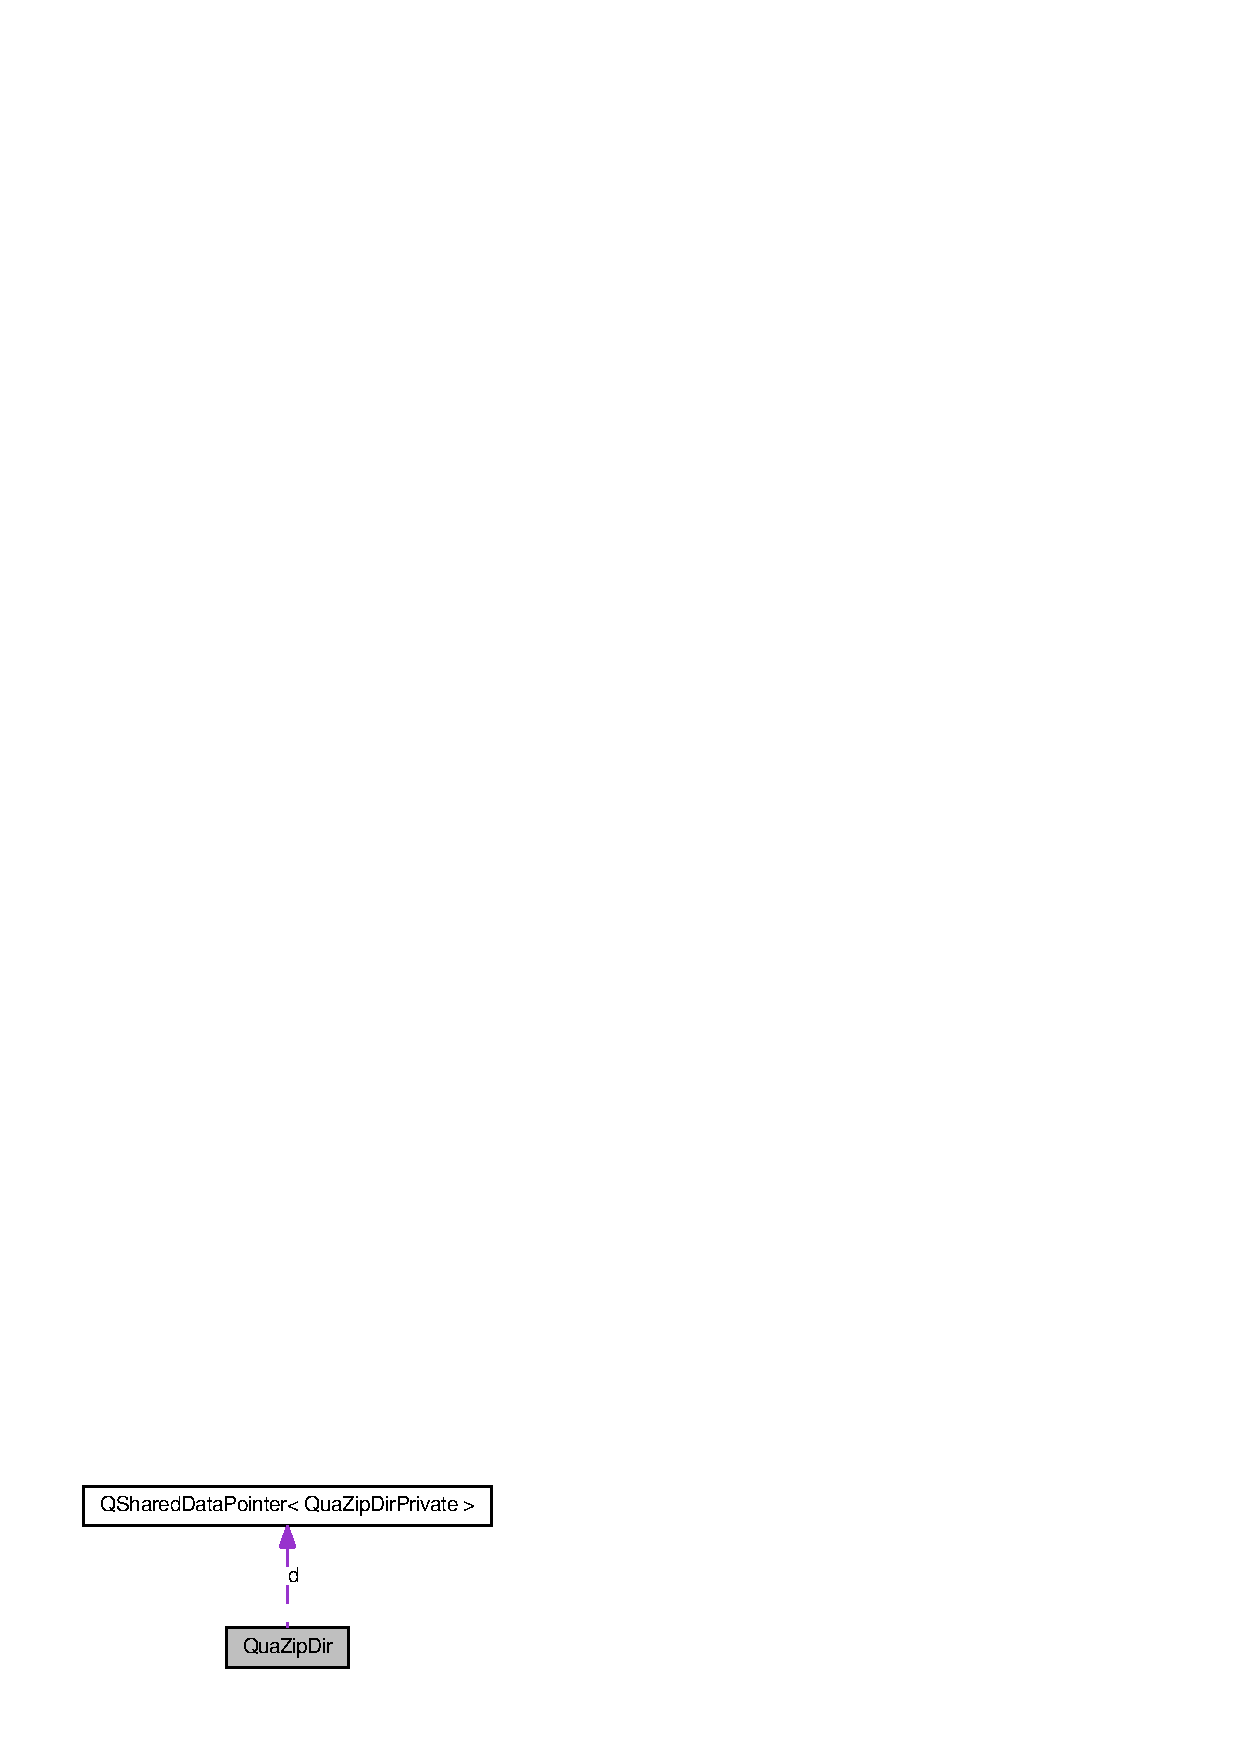
\includegraphics[width=240pt]{classQuaZipDir__coll__graph}
\end{center}
\end{figure}
\subsection*{Public Member Functions}
\begin{DoxyCompactItemize}
\item 
{\bf QuaZipDir} (const {\bf QuaZipDir} \&that)\label{classQuaZipDir_a6c9cc8b74c52d3fe997b753370566690}

\begin{DoxyCompactList}\small\item\em The copy constructor. \end{DoxyCompactList}\item 
{\bf QuaZipDir} ({\bf QuaZip} $\ast$zip, const {\bf QString} \&dir={\bf QString}())
\begin{DoxyCompactList}\small\item\em Constructs a \doxyref{QuaZipDir}{p.}{classQuaZipDir} instance pointing to the specified directory. \end{DoxyCompactList}\item 
{\bf $\sim$QuaZipDir} ()\label{classQuaZipDir_ae95d60e2c23e611723371bf8fff2b095}

\begin{DoxyCompactList}\small\item\em Destructor. \end{DoxyCompactList}\item 
bool {\bf operator==} (const {\bf QuaZipDir} \&that)\label{classQuaZipDir_a4a2e07484c7159a3f469922ba2383547}

\begin{DoxyCompactList}\small\item\em The assignment operator. \end{DoxyCompactList}\item 
bool {\bf operator!=} (const {\bf QuaZipDir} \&that)
\begin{DoxyCompactList}\small\item\em operator!= \end{DoxyCompactList}\item 
{\bf QuaZipDir} \& {\bf operator=} (const {\bf QuaZipDir} \&that)
\begin{DoxyCompactList}\small\item\em operator== \end{DoxyCompactList}\item 
{\bf QString} {\bf operator[$\,$]} (int pos) const \label{classQuaZipDir_a9e37ef5318c44a4575c58d66110e535a}

\begin{DoxyCompactList}\small\item\em Returns the name of the entry at the specified position. \end{DoxyCompactList}\item 
{\bf QuaZip::CaseSensitivity} {\bf caseSensitivity} () const \label{classQuaZipDir_ad7ab403a8d36a3b6149da86ea37178f8}

\begin{DoxyCompactList}\small\item\em Returns the current case sensitivity mode. \end{DoxyCompactList}\item 
bool {\bf cd} (const {\bf QString} \&dirName)
\begin{DoxyCompactList}\small\item\em Changes the 'current' directory. \end{DoxyCompactList}\item 
bool {\bf cdUp} ()\label{classQuaZipDir_a62306db3f4c0866930fa35c7348b84b3}

\begin{DoxyCompactList}\small\item\em Goes up. \end{DoxyCompactList}\item 
uint {\bf count} () const \label{classQuaZipDir_aa3f14665e3991351f4ef94ab8e0ab29d}

\begin{DoxyCompactList}\small\item\em Returns the number of entries in the directory. \end{DoxyCompactList}\item 
{\bf QString} {\bf dirName} () const 
\begin{DoxyCompactList}\small\item\em Returns the current directory name. \end{DoxyCompactList}\item 
{\bf QList}$<$ {\bf QuaZipFileInfo} $>$ {\bf entryInfoList} (const {\bf QStringList} \&nameFilters, {\bf QDir::Filters} filters=QDir::NoFilter, {\bf QDir::SortFlags} sort=QDir::NoSort) const 
\begin{DoxyCompactList}\small\item\em Returns the list of the entries in the directory. \end{DoxyCompactList}\item 
{\bf QList}$<$ {\bf QuaZipFileInfo} $>$ {\bf entryInfoList} ({\bf QDir::Filters} filters=QDir::NoFilter, {\bf QDir::SortFlags} sort=QDir::NoSort) const 
\begin{DoxyCompactList}\small\item\em Returns the list of the entries in the directory. \end{DoxyCompactList}\item 
{\bf QList}$<$ {\bf QuaZipFileInfo64} $>$ {\bf entryInfoList64} (const {\bf QStringList} \&nameFilters, {\bf QDir::Filters} filters=QDir::NoFilter, {\bf QDir::SortFlags} sort=QDir::NoSort) const 
\begin{DoxyCompactList}\small\item\em Returns the list of the entries in the directory with zip64 support. \end{DoxyCompactList}\item 
{\bf QList}$<$ {\bf QuaZipFileInfo64} $>$ {\bf entryInfoList64} ({\bf QDir::Filters} filters=QDir::NoFilter, {\bf QDir::SortFlags} sort=QDir::NoSort) const 
\begin{DoxyCompactList}\small\item\em Returns the list of the entries in the directory with zip64 support. \end{DoxyCompactList}\item 
{\bf QStringList} {\bf entryList} (const {\bf QStringList} \&nameFilters, {\bf QDir::Filters} filters=QDir::NoFilter, {\bf QDir::SortFlags} sort=QDir::NoSort) const 
\begin{DoxyCompactList}\small\item\em Returns the list of the entry names in the directory. \end{DoxyCompactList}\item 
{\bf QStringList} {\bf entryList} ({\bf QDir::Filters} filters=QDir::NoFilter, {\bf QDir::SortFlags} sort=QDir::NoSort) const 
\begin{DoxyCompactList}\small\item\em Returns the list of the entry names in the directory. \end{DoxyCompactList}\item 
bool {\bf exists} (const {\bf QString} \&fileName) const 
\begin{DoxyCompactList}\small\item\em Returns {\ttfamily true} if the entry with the specified name exists. \end{DoxyCompactList}\item 
bool {\bf exists} () const \label{classQuaZipDir_a22c8f63ce874f5c0e958ae5f42e6d004}

\begin{DoxyCompactList}\small\item\em Return {\ttfamily true} if the directory pointed by this \doxyref{QuaZipDir}{p.}{classQuaZipDir} exists. \end{DoxyCompactList}\item 
{\bf QString} {\bf filePath} (const {\bf QString} \&fileName) const 
\begin{DoxyCompactList}\small\item\em Returns the full path to the specified file. \end{DoxyCompactList}\item 
{\bf QDir::Filters} {\bf filter} ()\label{classQuaZipDir_abeee1810c7c1c1af93364081dbf70d38}

\begin{DoxyCompactList}\small\item\em Returns the default filter. \end{DoxyCompactList}\item 
bool {\bf isRoot} () const 
\begin{DoxyCompactList}\small\item\em Returns if the \doxyref{QuaZipDir}{p.}{classQuaZipDir} points to the root of the archive. \end{DoxyCompactList}\item 
{\bf QStringList} {\bf nameFilters} () const \label{classQuaZipDir_a00f18e23abb8cac04f975e7f31553f2e}

\begin{DoxyCompactList}\small\item\em Return the default name filter. \end{DoxyCompactList}\item 
{\bf QString} {\bf path} () const 
\begin{DoxyCompactList}\small\item\em Returns the path to the current dir. \end{DoxyCompactList}\item 
{\bf QString} {\bf relativeFilePath} (const {\bf QString} \&fileName) const 
\begin{DoxyCompactList}\small\item\em Returns the path to the specified file relative to the current dir. \end{DoxyCompactList}\item 
void {\bf setCaseSensitivity} ({\bf QuaZip::CaseSensitivity} caseSensitivity)\label{classQuaZipDir_ad53c720975bb0c49a823355f7d518793}

\begin{DoxyCompactList}\small\item\em Sets the default case sensitivity mode. \end{DoxyCompactList}\item 
void {\bf setFilter} ({\bf QDir::Filters} filters)\label{classQuaZipDir_a779a43641f0f3802678e39c9acd1fddb}

\begin{DoxyCompactList}\small\item\em Sets the default filter. \end{DoxyCompactList}\item 
void {\bf setNameFilters} (const {\bf QStringList} \&nameFilters)\label{classQuaZipDir_abcf208bfd6136e14f36725ae79dce2be}

\begin{DoxyCompactList}\small\item\em Sets the default name filter. \end{DoxyCompactList}\item 
void {\bf setPath} (const {\bf QString} \&path)
\begin{DoxyCompactList}\small\item\em Goes to the specified path. \end{DoxyCompactList}\item 
void {\bf setSorting} ({\bf QDir::SortFlags} sort)\label{classQuaZipDir_ae43e9d717e3c4b1c0d4790cf558e7451}

\begin{DoxyCompactList}\small\item\em Sets the default sorting mode. \end{DoxyCompactList}\item 
{\bf QDir::SortFlags} {\bf sorting} () const \label{classQuaZipDir_a4000523c961ab9e0cad08641ff10e3fa}

\begin{DoxyCompactList}\small\item\em Returns the default sorting mode. \end{DoxyCompactList}\end{DoxyCompactItemize}


\subsection{Detailed Description}
Provides ZIP archive navigation. 

This class is modelled after {\bf QDir}, and is designed to provide similar features for ZIP archives.

The only significant difference from {\bf QDir} is that the root path is not '/', but an empty string since that's how the file paths are stored in the archive. However, \doxyref{QuaZipDir}{p.}{classQuaZipDir} understands the paths starting with '/'. It is important in a few places:


\begin{DoxyItemize}
\item In the \doxyref{cd()}{p.}{classQuaZipDir_aa829afc0243f1d307302f1167edecc7b} function.
\item In the constructor.
\item In the \doxyref{exists()}{p.}{classQuaZipDir_aacb488fec6e951ac80e5d473534fee97} function.
\item In the relativePath() function.
\end{DoxyItemize}

Note that since ZIP uses '/' on all platforms, the '$\backslash$' separator is not supported. 

\subsection{Constructor \& Destructor Documentation}
\index{QuaZipDir@{QuaZipDir}!QuaZipDir@{QuaZipDir}}
\index{QuaZipDir@{QuaZipDir}!QuaZipDir@{QuaZipDir}}
\subsubsection[{QuaZipDir}]{\setlength{\rightskip}{0pt plus 5cm}QuaZipDir::QuaZipDir (
\begin{DoxyParamCaption}
\item[{{\bf QuaZip} $\ast$}]{zip, }
\item[{const {\bf QString} \&}]{dir = {\ttfamily {\bf QString}()}}
\end{DoxyParamCaption}
)}\label{classQuaZipDir_a19e5e3a54f322ce03e7f7606a87a2ba1}


Constructs a \doxyref{QuaZipDir}{p.}{classQuaZipDir} instance pointing to the specified directory. 

If {\itshape dir\/} is not specified, points to the root of the archive. The same happens if the {\itshape dir\/} is "/". 

\subsection{Member Function Documentation}
\index{QuaZipDir@{QuaZipDir}!operator!=@{operator!=}}
\index{operator!=@{operator!=}!QuaZipDir@{QuaZipDir}}
\subsubsection[{operator!=}]{\setlength{\rightskip}{0pt plus 5cm}bool QuaZipDir::operator!= (
\begin{DoxyParamCaption}
\item[{const {\bf QuaZipDir} \&}]{that}
\end{DoxyParamCaption}
)\hspace{0.3cm}{\ttfamily  [inline]}}\label{classQuaZipDir_a6e60d858d05774c958215ee7741eceed}


operator!= 

\begin{DoxyReturn}{Returns}
{\ttfamily true} if either this and {\itshape that\/} use different \doxyref{QuaZip}{p.}{classQuaZip} instances or if they point to different directories. 
\end{DoxyReturn}
\index{QuaZipDir@{QuaZipDir}!operator=@{operator=}}
\index{operator=@{operator=}!QuaZipDir@{QuaZipDir}}
\subsubsection[{operator=}]{\setlength{\rightskip}{0pt plus 5cm}{\bf QuaZipDir} \& QuaZipDir::operator= (
\begin{DoxyParamCaption}
\item[{const {\bf QuaZipDir} \&}]{that}
\end{DoxyParamCaption}
)}\label{classQuaZipDir_aa603c69be0c1597add5951b19f8bc961}


operator== 

\begin{DoxyReturn}{Returns}
{\ttfamily true} if both this and {\itshape that\/} use the same \doxyref{QuaZip}{p.}{classQuaZip} instance and point to the same directory. 
\end{DoxyReturn}
\index{QuaZipDir@{QuaZipDir}!cd@{cd}}
\index{cd@{cd}!QuaZipDir@{QuaZipDir}}
\subsubsection[{cd}]{\setlength{\rightskip}{0pt plus 5cm}bool QuaZipDir::cd (
\begin{DoxyParamCaption}
\item[{const {\bf QString} \&}]{dirName}
\end{DoxyParamCaption}
)}\label{classQuaZipDir_aa829afc0243f1d307302f1167edecc7b}


Changes the 'current' directory. 

If the path starts with '/', it is interpreted as an absolute path from the root of the archive. Otherwise, it is interpreted as a path relative to the current directory as was set by the previous \doxyref{cd()}{p.}{classQuaZipDir_aa829afc0243f1d307302f1167edecc7b} or the constructor.

Note that the subsequent \doxyref{path()}{p.}{classQuaZipDir_a68ac82ad605c0b10f9ee1a2d6d474f52} call will not return a path starting with '/' in all cases. 

References cd(), QString::chop(), QList::constBegin(), QByteArray::constData(), QString::contains(), dirName(), QList::end(), QString::endsWith(), exists(), isRoot(), path(), QString::split(), QString::startsWith(), and QString::toUtf8().



Referenced by cd(), and cdUp().

\index{QuaZipDir@{QuaZipDir}!dirName@{dirName}}
\index{dirName@{dirName}!QuaZipDir@{QuaZipDir}}
\subsubsection[{dirName}]{\setlength{\rightskip}{0pt plus 5cm}{\bf QString} QuaZipDir::dirName (
\begin{DoxyParamCaption}
{}
\end{DoxyParamCaption}
) const}\label{classQuaZipDir_afd2f76410f7728a7166b7598926fbf96}


Returns the current directory name. 

The name doesn't include the path. 

References QDir::dirName().



Referenced by cd().

\index{QuaZipDir@{QuaZipDir}!entryInfoList@{entryInfoList}}
\index{entryInfoList@{entryInfoList}!QuaZipDir@{QuaZipDir}}
\subsubsection[{entryInfoList}]{\setlength{\rightskip}{0pt plus 5cm}{\bf QList}$<$ {\bf QuaZipFileInfo} $>$ QuaZipDir::entryInfoList (
\begin{DoxyParamCaption}
\item[{const {\bf QStringList} \&}]{nameFilters, }
\item[{{\bf QDir::Filters}}]{filters = {\ttfamily QDir::NoFilter}, }
\item[{{\bf QDir::SortFlags}}]{sort = {\ttfamily QDir::NoSort}}
\end{DoxyParamCaption}
) const}\label{classQuaZipDir_aef966735a146fc10c9527c236aa89261}


Returns the list of the entries in the directory. 


\begin{DoxyParams}{Parameters}
{\em nameFilters} & The list of file patterns to list, uses the same syntax as {\bf QDir}. \\
\hline
{\em filters} & The entry type filters, only Files and Dirs are accepted. \\
\hline
{\em sort} & Sorting mode.\\
\hline
\end{DoxyParams}


Referenced by entryInfoList().

\index{QuaZipDir@{QuaZipDir}!entryInfoList@{entryInfoList}}
\index{entryInfoList@{entryInfoList}!QuaZipDir@{QuaZipDir}}
\subsubsection[{entryInfoList}]{\setlength{\rightskip}{0pt plus 5cm}{\bf QList}$<$ {\bf QuaZipFileInfo} $>$ QuaZipDir::entryInfoList (
\begin{DoxyParamCaption}
\item[{{\bf QDir::Filters}}]{filters = {\ttfamily QDir::NoFilter}, }
\item[{{\bf QDir::SortFlags}}]{sort = {\ttfamily QDir::NoSort}}
\end{DoxyParamCaption}
) const}\label{classQuaZipDir_abec530f15597ddf8c8d1f340a333f7aa}


Returns the list of the entries in the directory. 

This is an overloaded member function, provided for convenience. It differs from the above function only in what argument(s) it accepts. The same as entryInfoList(QStringList(), filters, sort). 

References entryInfoList().

\index{QuaZipDir@{QuaZipDir}!entryInfoList64@{entryInfoList64}}
\index{entryInfoList64@{entryInfoList64}!QuaZipDir@{QuaZipDir}}
\subsubsection[{entryInfoList64}]{\setlength{\rightskip}{0pt plus 5cm}{\bf QList}$<$ {\bf QuaZipFileInfo64} $>$ QuaZipDir::entryInfoList64 (
\begin{DoxyParamCaption}
\item[{const {\bf QStringList} \&}]{nameFilters, }
\item[{{\bf QDir::Filters}}]{filters = {\ttfamily QDir::NoFilter}, }
\item[{{\bf QDir::SortFlags}}]{sort = {\ttfamily QDir::NoSort}}
\end{DoxyParamCaption}
) const}\label{classQuaZipDir_ae2b5a4b251db7aeb165c6656da0e3431}


Returns the list of the entries in the directory with zip64 support. 


\begin{DoxyParams}{Parameters}
{\em nameFilters} & The list of file patterns to list, uses the same syntax as {\bf QDir}. \\
\hline
{\em filters} & The entry type filters, only Files and Dirs are accepted. \\
\hline
{\em sort} & Sorting mode. \\
\hline
\end{DoxyParams}


Referenced by entryInfoList64().

\index{QuaZipDir@{QuaZipDir}!entryInfoList64@{entryInfoList64}}
\index{entryInfoList64@{entryInfoList64}!QuaZipDir@{QuaZipDir}}
\subsubsection[{entryInfoList64}]{\setlength{\rightskip}{0pt plus 5cm}{\bf QList}$<$ {\bf QuaZipFileInfo64} $>$ QuaZipDir::entryInfoList64 (
\begin{DoxyParamCaption}
\item[{{\bf QDir::Filters}}]{filters = {\ttfamily QDir::NoFilter}, }
\item[{{\bf QDir::SortFlags}}]{sort = {\ttfamily QDir::NoSort}}
\end{DoxyParamCaption}
) const}\label{classQuaZipDir_a8c38ec214c300049685cbf71486636d5}


Returns the list of the entries in the directory with zip64 support. 

This is an overloaded member function, provided for convenience. It differs from the above function only in what argument(s) it accepts. The same as entryInfoList64(QStringList(), filters, sort). 

References entryInfoList64().

\index{QuaZipDir@{QuaZipDir}!entryList@{entryList}}
\index{entryList@{entryList}!QuaZipDir@{QuaZipDir}}
\subsubsection[{entryList}]{\setlength{\rightskip}{0pt plus 5cm}{\bf QStringList} QuaZipDir::entryList (
\begin{DoxyParamCaption}
\item[{const {\bf QStringList} \&}]{nameFilters, }
\item[{{\bf QDir::Filters}}]{filters = {\ttfamily QDir::NoFilter}, }
\item[{{\bf QDir::SortFlags}}]{sort = {\ttfamily QDir::NoSort}}
\end{DoxyParamCaption}
) const}\label{classQuaZipDir_a4a32faa77c4120cd3c6db4b683fa16d9}


Returns the list of the entry names in the directory. 

The same as entryInfoList(nameFilters, filters, sort), but only returns entry names. 

Referenced by count(), entryList(), exists(), and operator[$\,$]().

\index{QuaZipDir@{QuaZipDir}!entryList@{entryList}}
\index{entryList@{entryList}!QuaZipDir@{QuaZipDir}}
\subsubsection[{entryList}]{\setlength{\rightskip}{0pt plus 5cm}{\bf QStringList} QuaZipDir::entryList (
\begin{DoxyParamCaption}
\item[{{\bf QDir::Filters}}]{filters = {\ttfamily QDir::NoFilter}, }
\item[{{\bf QDir::SortFlags}}]{sort = {\ttfamily QDir::NoSort}}
\end{DoxyParamCaption}
) const}\label{classQuaZipDir_ab20e9d3de675b74fcacc98accbc1d766}


Returns the list of the entry names in the directory. 

This is an overloaded member function, provided for convenience. It differs from the above function only in what argument(s) it accepts. The same as entryList(QStringList(), filters, sort). 

References entryList().

\index{QuaZipDir@{QuaZipDir}!exists@{exists}}
\index{exists@{exists}!QuaZipDir@{QuaZipDir}}
\subsubsection[{exists}]{\setlength{\rightskip}{0pt plus 5cm}bool QuaZipDir::exists (
\begin{DoxyParamCaption}
\item[{const {\bf QString} \&}]{fileName}
\end{DoxyParamCaption}
) const}\label{classQuaZipDir_aacb488fec6e951ac80e5d473534fee97}


Returns {\ttfamily true} if the entry with the specified name exists. 

The ".." is considered to exist if the current directory is not root. The "." and "/" are considered to always exist. Paths starting with "/" are relative to the archive root, other paths are relative to the current dir. 

References QString::chop(), QList::constBegin(), QByteArray::constData(), QList::constEnd(), QStringList::contains(), QString::contains(), QuaZip::convertCaseSensitivity(), QString::endsWith(), entryList(), QFileInfo::fileName(), filePath(), QString::isEmpty(), isRoot(), QFileInfo::path(), and QString::toUtf8().

\index{QuaZipDir@{QuaZipDir}!filePath@{filePath}}
\index{filePath@{filePath}!QuaZipDir@{QuaZipDir}}
\subsubsection[{filePath}]{\setlength{\rightskip}{0pt plus 5cm}{\bf QString} QuaZipDir::filePath (
\begin{DoxyParamCaption}
\item[{const {\bf QString} \&}]{fileName}
\end{DoxyParamCaption}
) const}\label{classQuaZipDir_ae8b576a150f8d62c902067603cbc97ae}


Returns the full path to the specified file. 

Doesn't check if the file actually exists. 

References QDir::filePath().



Referenced by exists().

\index{QuaZipDir@{QuaZipDir}!isRoot@{isRoot}}
\index{isRoot@{isRoot}!QuaZipDir@{QuaZipDir}}
\subsubsection[{isRoot}]{\setlength{\rightskip}{0pt plus 5cm}bool QuaZipDir::isRoot (
\begin{DoxyParamCaption}
{}
\end{DoxyParamCaption}
) const}\label{classQuaZipDir_a598fdf23f1b37e1876476e5969040a32}


Returns if the \doxyref{QuaZipDir}{p.}{classQuaZipDir} points to the root of the archive. 

Not that the root path is the empty string, not '/'. 

Referenced by cd(), and exists().

\index{QuaZipDir@{QuaZipDir}!path@{path}}
\index{path@{path}!QuaZipDir@{QuaZipDir}}
\subsubsection[{path}]{\setlength{\rightskip}{0pt plus 5cm}{\bf QString} QuaZipDir::path (
\begin{DoxyParamCaption}
{}
\end{DoxyParamCaption}
) const}\label{classQuaZipDir_a68ac82ad605c0b10f9ee1a2d6d474f52}


Returns the path to the current dir. 

The path never starts with '/', and the root path is an empty string. 

Referenced by cd(), and setPath().

\index{QuaZipDir@{QuaZipDir}!relativeFilePath@{relativeFilePath}}
\index{relativeFilePath@{relativeFilePath}!QuaZipDir@{QuaZipDir}}
\subsubsection[{relativeFilePath}]{\setlength{\rightskip}{0pt plus 5cm}{\bf QString} QuaZipDir::relativeFilePath (
\begin{DoxyParamCaption}
\item[{const {\bf QString} \&}]{fileName}
\end{DoxyParamCaption}
) const}\label{classQuaZipDir_a2ae89c2b85786a0168656fc7a3faaf01}


Returns the path to the specified file relative to the current dir. 

This function is mostly useless, provided only for the sake of completeness.


\begin{DoxyParams}{Parameters}
{\em fileName} & The path to the file, should start with "/" if relative to the archive root. \\
\hline
\end{DoxyParams}
\begin{DoxyReturn}{Returns}
Path relative to the current dir. 
\end{DoxyReturn}


References QDir::relativeFilePath().

\index{QuaZipDir@{QuaZipDir}!setPath@{setPath}}
\index{setPath@{setPath}!QuaZipDir@{QuaZipDir}}
\subsubsection[{setPath}]{\setlength{\rightskip}{0pt plus 5cm}void QuaZipDir::setPath (
\begin{DoxyParamCaption}
\item[{const {\bf QString} \&}]{path}
\end{DoxyParamCaption}
)}\label{classQuaZipDir_ae82d06e43856414c30583205d337c111}


Goes to the specified path. 

The difference from \doxyref{cd()}{p.}{classQuaZipDir_aa829afc0243f1d307302f1167edecc7b} is that this function never checks if the path actually exists and doesn't use relative paths, so it's possible to go to the root directory with setPath("").

Note that this function still chops the trailing and/or leading '/' and treats a single '/' as the root path (\doxyref{path()}{p.}{classQuaZipDir_a68ac82ad605c0b10f9ee1a2d6d474f52} will still return an empty string). 

References QString::chop(), QString::endsWith(), QString::mid(), path(), and QString::startsWith().



The documentation for this class was generated from the following files:\begin{DoxyCompactItemize}
\item 
quazip/quazipdir.h\item 
quazip/quazipdir.cpp\end{DoxyCompactItemize}

\section{QuaZipFile Class Reference}
\label{classQuaZipFile}\index{QuaZipFile@{QuaZipFile}}


A file inside ZIP archive.  




{\ttfamily \#include $<$quazip/quazipfile.h$>$}



Inheritance diagram for QuaZipFile:
\nopagebreak
\begin{figure}[H]
\begin{center}
\leavevmode
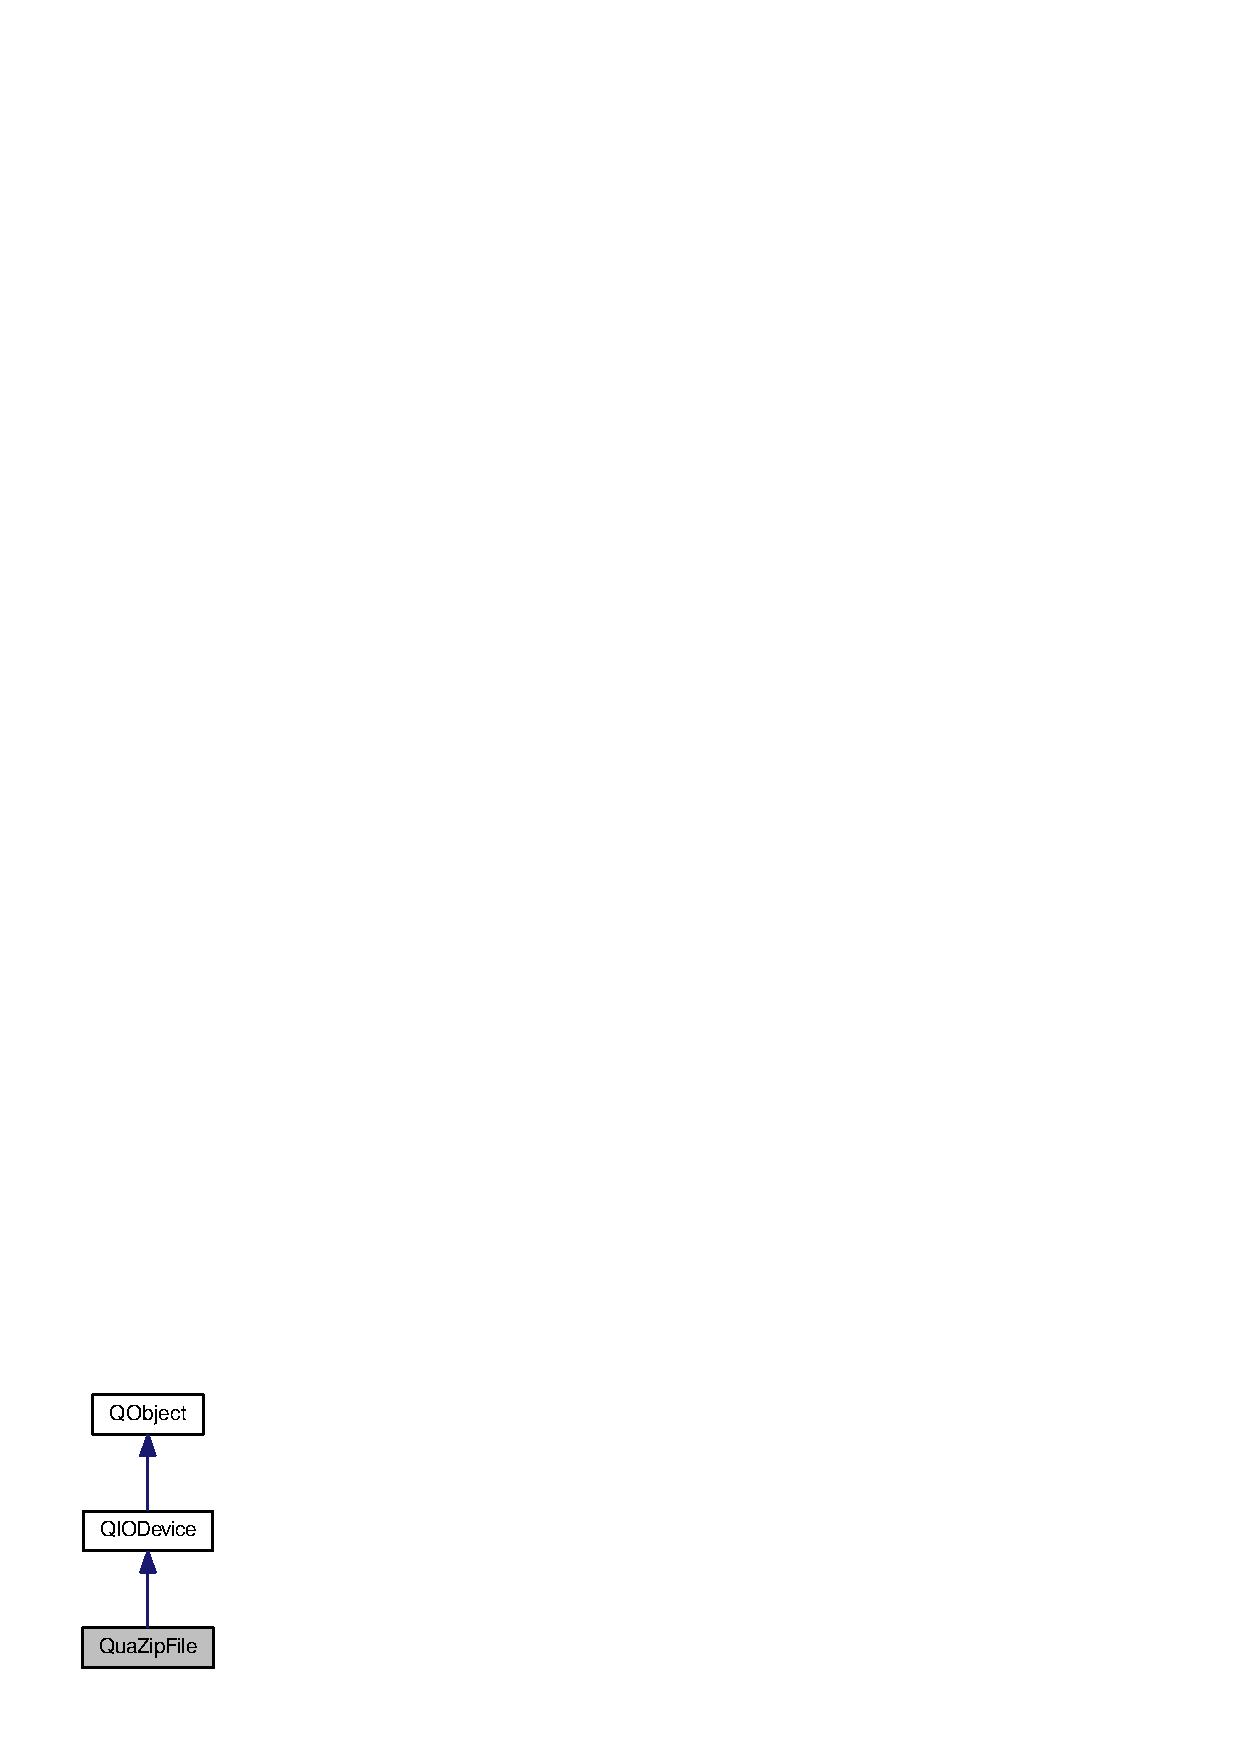
\includegraphics[width=106pt]{classQuaZipFile__inherit__graph}
\end{center}
\end{figure}


Collaboration diagram for QuaZipFile:
\nopagebreak
\begin{figure}[H]
\begin{center}
\leavevmode
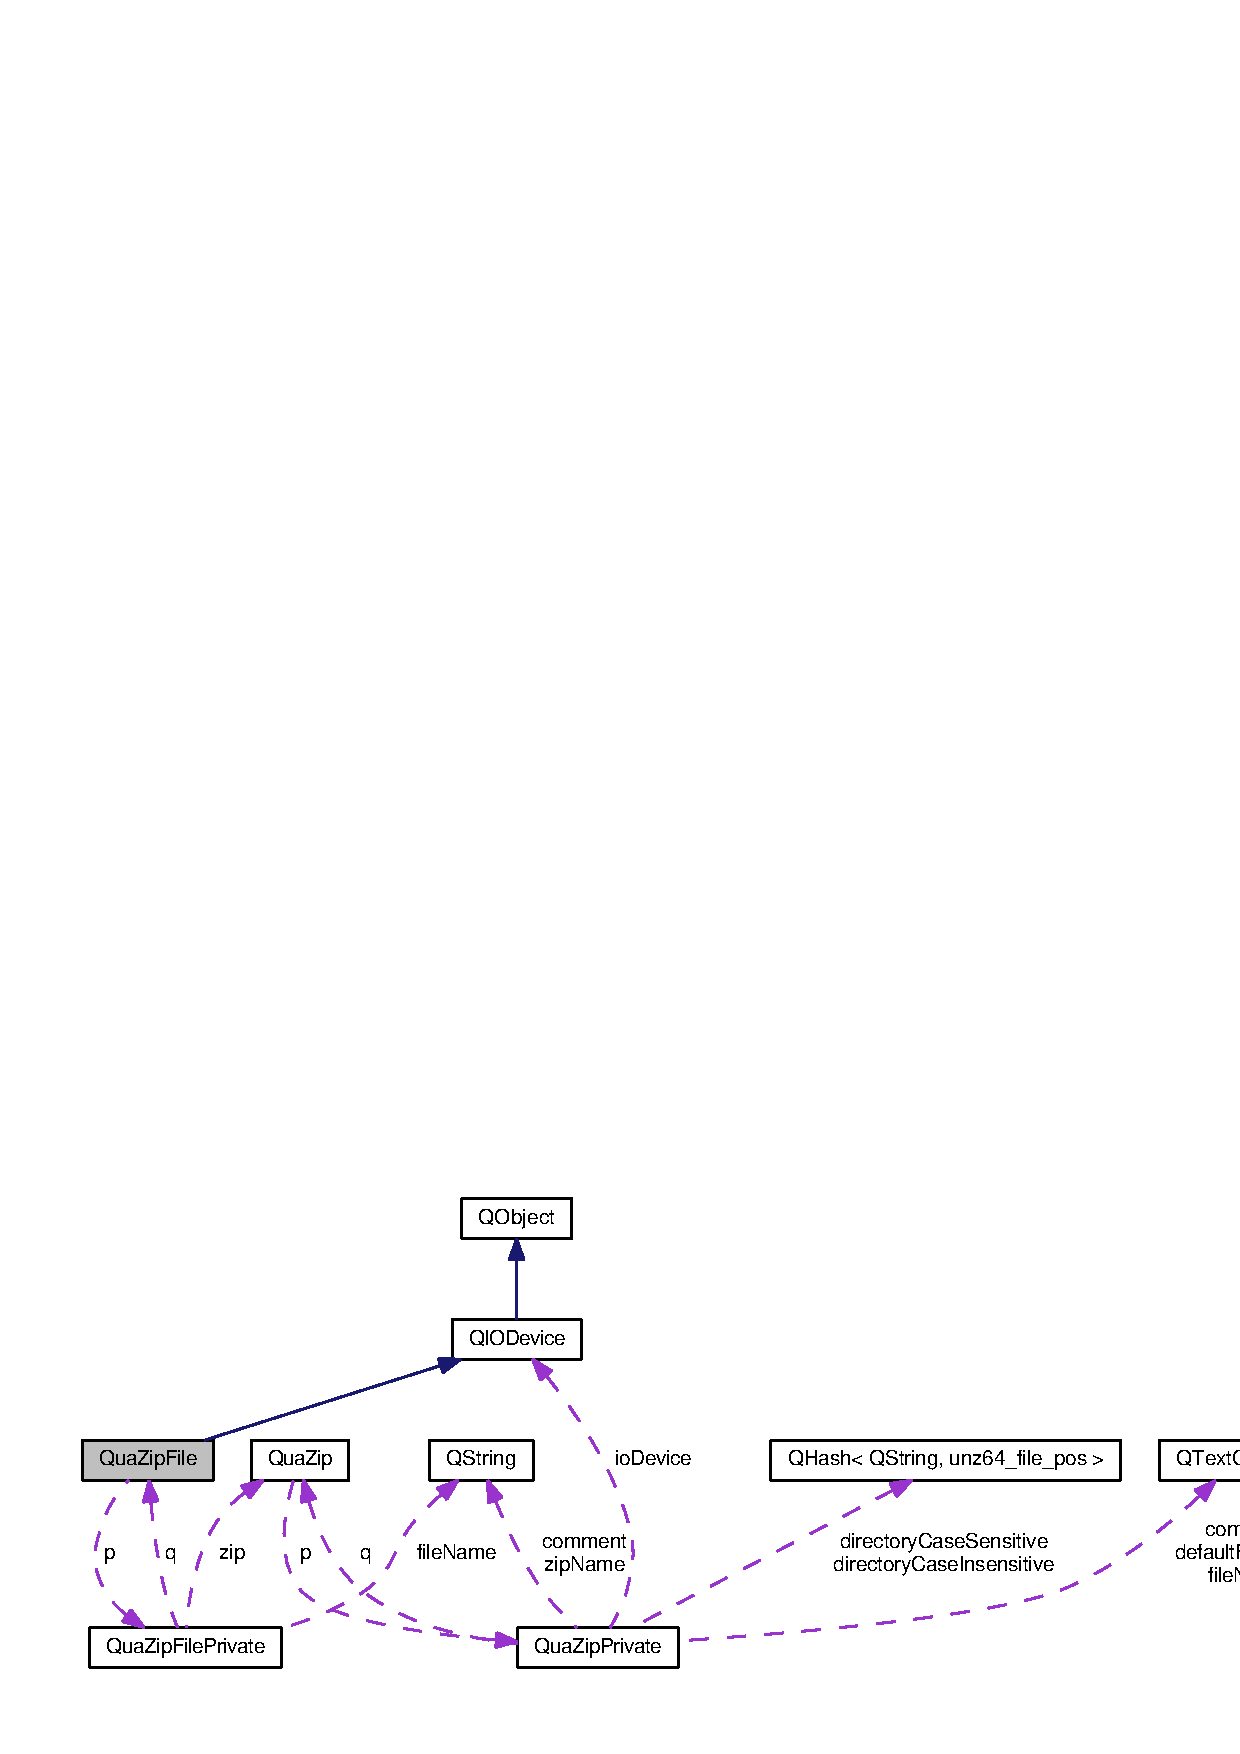
\includegraphics[width=400pt]{classQuaZipFile__coll__graph}
\end{center}
\end{figure}
\subsection*{Public Member Functions}
\begin{DoxyCompactItemize}
\item 
{\bf QuaZipFile} ()
\begin{DoxyCompactList}\small\item\em Constructs a \doxyref{QuaZipFile}{p.}{classQuaZipFile} instance. \end{DoxyCompactList}\item 
{\bf QuaZipFile} ({\bf QObject} $\ast${\bf parent})
\begin{DoxyCompactList}\small\item\em Constructs a \doxyref{QuaZipFile}{p.}{classQuaZipFile} instance. \end{DoxyCompactList}\item 
{\bf QuaZipFile} (const {\bf QString} \&zipName, {\bf QObject} $\ast${\bf parent}=NULL)
\begin{DoxyCompactList}\small\item\em Constructs a \doxyref{QuaZipFile}{p.}{classQuaZipFile} instance. \end{DoxyCompactList}\item 
{\bf QuaZipFile} (const {\bf QString} \&zipName, const {\bf QString} \&fileName, {\bf QuaZip::CaseSensitivity} cs=QuaZip::csDefault, {\bf QObject} $\ast${\bf parent}=NULL)
\begin{DoxyCompactList}\small\item\em Constructs a \doxyref{QuaZipFile}{p.}{classQuaZipFile} instance. \end{DoxyCompactList}\item 
{\bf QuaZipFile} ({\bf QuaZip} $\ast$zip, {\bf QObject} $\ast${\bf parent}=NULL)
\begin{DoxyCompactList}\small\item\em Constructs a \doxyref{QuaZipFile}{p.}{classQuaZipFile} instance. \end{DoxyCompactList}\item 
virtual {\bf $\sim$QuaZipFile} ()
\begin{DoxyCompactList}\small\item\em Destroys a \doxyref{QuaZipFile}{p.}{classQuaZipFile} instance. \end{DoxyCompactList}\item 
{\bf QString} {\bf getZipName} () const 
\begin{DoxyCompactList}\small\item\em Returns the ZIP archive file name. \end{DoxyCompactList}\item 
{\bf QuaZip} $\ast$ {\bf getZip} () const 
\begin{DoxyCompactList}\small\item\em Returns a pointer to the associated \doxyref{QuaZip}{p.}{classQuaZip} object. \end{DoxyCompactList}\item 
{\bf QString} {\bf getFileName} () const 
\begin{DoxyCompactList}\small\item\em Returns file name. \end{DoxyCompactList}\item 
{\bf QuaZip::CaseSensitivity} {\bf getCaseSensitivity} () const 
\begin{DoxyCompactList}\small\item\em Returns case sensitivity of the file name. \end{DoxyCompactList}\item 
{\bf QString} {\bf getActualFileName} () const 
\begin{DoxyCompactList}\small\item\em Returns the actual file name in the archive. \end{DoxyCompactList}\item 
void {\bf setZipName} (const {\bf QString} \&zipName)
\begin{DoxyCompactList}\small\item\em Sets the ZIP archive file name. \end{DoxyCompactList}\item 
bool {\bf isRaw} () const 
\begin{DoxyCompactList}\small\item\em Returns {\ttfamily true} if the file was opened in raw mode. \end{DoxyCompactList}\item 
void {\bf setZip} ({\bf QuaZip} $\ast$zip)
\begin{DoxyCompactList}\small\item\em Binds to the existing \doxyref{QuaZip}{p.}{classQuaZip} instance. \end{DoxyCompactList}\item 
void {\bf setFileName} (const {\bf QString} \&fileName, {\bf QuaZip::CaseSensitivity} cs=QuaZip::csDefault)
\begin{DoxyCompactList}\small\item\em Sets the file name. \end{DoxyCompactList}\item 
virtual bool {\bf open} ({\bf OpenMode} mode)
\begin{DoxyCompactList}\small\item\em Opens a file for reading. \end{DoxyCompactList}\item 
bool {\bf open} ({\bf OpenMode} mode, const char $\ast$password)
\begin{DoxyCompactList}\small\item\em Opens a file for reading. \end{DoxyCompactList}\item 
bool {\bf open} ({\bf OpenMode} mode, int $\ast$method, int $\ast$level, bool raw, const char $\ast$password=NULL)
\begin{DoxyCompactList}\small\item\em Opens a file for reading. \end{DoxyCompactList}\item 
bool {\bf open} ({\bf OpenMode} mode, const {\bf QuaZipNewInfo} \&info, const char $\ast$password=NULL, quint32 crc=0, int method=Z\_\-DEFLATED, int level=Z\_\-DEFAULT\_\-COMPRESSION, bool raw=false, int windowBits=-\/MAX\_\-WBITS, int memLevel=DEF\_\-MEM\_\-LEVEL, int strategy=Z\_\-DEFAULT\_\-STRATEGY)
\begin{DoxyCompactList}\small\item\em Opens a file for writing. \end{DoxyCompactList}\item 
virtual bool {\bf isSequential} () const \label{classQuaZipFile_a64430ec50820c8096f963a7e5f53001f}

\begin{DoxyCompactList}\small\item\em Returns {\ttfamily true}, but \doxyref{beware}{p.}{classQuaZipFile_quazipfile-sequential}! \end{DoxyCompactList}\item 
virtual qint64 {\bf pos} () const 
\begin{DoxyCompactList}\small\item\em Returns current position in the file. \end{DoxyCompactList}\item 
virtual bool {\bf atEnd} () const 
\begin{DoxyCompactList}\small\item\em Returns {\ttfamily true} if the end of file was reached. \end{DoxyCompactList}\item 
virtual qint64 {\bf size} () const 
\begin{DoxyCompactList}\small\item\em Returns file size. \end{DoxyCompactList}\item 
qint64 {\bf csize} () const 
\begin{DoxyCompactList}\small\item\em Returns compressed file size. \end{DoxyCompactList}\item 
qint64 {\bf usize} () const 
\begin{DoxyCompactList}\small\item\em Returns uncompressed file size. \end{DoxyCompactList}\item 
bool {\bf getFileInfo} ({\bf QuaZipFileInfo} $\ast$info)
\begin{DoxyCompactList}\small\item\em Gets information about current file. \end{DoxyCompactList}\item 
bool {\bf getFileInfo} ({\bf QuaZipFileInfo64} $\ast$info)
\begin{DoxyCompactList}\small\item\em Gets information about current file with zip64 support. \end{DoxyCompactList}\item 
virtual void {\bf close} ()
\begin{DoxyCompactList}\small\item\em Closes the file. \end{DoxyCompactList}\item 
int {\bf getZipError} () const \label{classQuaZipFile_a26d2ee56aad947193b73052f80597ef0}

\begin{DoxyCompactList}\small\item\em Returns the error code returned by the last ZIP/UNZIP API call. \end{DoxyCompactList}\item 
virtual qint64 {\bf bytesAvailable} () const \label{classQuaZipFile_a29fbfb34677f69394ae7c986ffd3a0c1}

\begin{DoxyCompactList}\small\item\em Returns the number of bytes available for reading. \end{DoxyCompactList}\end{DoxyCompactItemize}
\subsection*{Protected Member Functions}
\begin{DoxyCompactItemize}
\item 
qint64 {\bf readData} (char $\ast$data, qint64 maxSize)\label{classQuaZipFile_aa1f2274e1579327855a17d67a9046ec2}

\begin{DoxyCompactList}\small\item\em Implementation of the {\bf QIODevice::readData()}. \end{DoxyCompactList}\item 
qint64 {\bf writeData} (const char $\ast$data, qint64 maxSize)\label{classQuaZipFile_abd07949a6fcc2ef094d2be5398bc8e7c}

\begin{DoxyCompactList}\small\item\em Implementation of the {\bf QIODevice::writeData()}. \end{DoxyCompactList}\end{DoxyCompactItemize}
\subsection*{Friends}
\begin{DoxyCompactItemize}
\item 
class {\bf QuaZipFilePrivate}\label{classQuaZipFile_abeded291f2788ca39fe2256d78f95266}

\end{DoxyCompactItemize}


\subsection{Detailed Description}
A file inside ZIP archive. 

This is the most interesting class. Not only it provides C++ interface to the ZIP/UNZIP package, but also integrates it with {\bf Qt} by subclassing {\bf QIODevice}. This makes possible to access files inside ZIP archive using {\bf QTextStream} or {\bf QDataStream}, for example. Actually, this is the main purpose of the whole QuaZIP library.

You can either use existing \doxyref{QuaZip}{p.}{classQuaZip} instance to create instance of this class or pass ZIP archive file name to this class, in which case it will create internal \doxyref{QuaZip}{p.}{classQuaZip} object. See constructors' descriptions for details. Writing is only possible with the existing instance.

Note that due to the underlying library's limitation it is not possible to use multiple \doxyref{QuaZipFile}{p.}{classQuaZipFile} instances to open several files in the same archive at the same time. If you need to write to multiple files in parallel, then you should write to temporary files first, then pack them all at once when you have finished writing. If you need to read multiple files inside the same archive in parallel, you should extract them all into a temporary directory first.\subsection{Sequential or random-\/access?}\label{classQuaZipFile_quazipfile-sequential}
At the first thought, \doxyref{QuaZipFile}{p.}{classQuaZipFile} has fixed size, the start and the end and should be therefore considered random-\/access device. But there is one major obstacle to making it random-\/access: ZIP/UNZIP API does not support {\bf seek()} operation and the only way to implement it is through reopening the file and re-\/reading to the required position, but this is prohibitively slow.

Therefore, \doxyref{QuaZipFile}{p.}{classQuaZipFile} is considered to be a sequential device. This has advantage of availability of the {\bf ungetChar()} operation ({\bf QIODevice} does not implement it properly for non-\/sequential devices unless they support {\bf seek()}). Disadvantage is a somewhat strange behaviour of the \doxyref{size()}{p.}{classQuaZipFile_ad1a17cc690a01c3edfb82984c3a4c8f0} and \doxyref{pos()}{p.}{classQuaZipFile_a90fd55dab83eca7f95df50b2c41b7f22} functions. This should be kept in mind while using this class. 

\subsection{Constructor \& Destructor Documentation}
\index{QuaZipFile@{QuaZipFile}!QuaZipFile@{QuaZipFile}}
\index{QuaZipFile@{QuaZipFile}!QuaZipFile@{QuaZipFile}}
\subsubsection[{QuaZipFile}]{\setlength{\rightskip}{0pt plus 5cm}QuaZipFile::QuaZipFile (
\begin{DoxyParamCaption}
{}
\end{DoxyParamCaption}
)}\label{classQuaZipFile_ad31592e0e8a9eaa009c6c0e2040a2158}


Constructs a \doxyref{QuaZipFile}{p.}{classQuaZipFile} instance. 

You should use \doxyref{setZipName()}{p.}{classQuaZipFile_ac8109e9a5c19bea75982ff6986b5cb1e} and \doxyref{setFileName()}{p.}{classQuaZipFile_a3732ca7704379d457b6a27db8837de95} or \doxyref{setZip()}{p.}{classQuaZipFile_ab7939a26d1e8de2f6aca54f49a12b980} before trying to call \doxyref{open()}{p.}{classQuaZipFile_a4c20c0ef00ae79c9a59eafe2906c9384} on the constructed object. \index{QuaZipFile@{QuaZipFile}!QuaZipFile@{QuaZipFile}}
\index{QuaZipFile@{QuaZipFile}!QuaZipFile@{QuaZipFile}}
\subsubsection[{QuaZipFile}]{\setlength{\rightskip}{0pt plus 5cm}QuaZipFile::QuaZipFile (
\begin{DoxyParamCaption}
\item[{{\bf QObject} $\ast$}]{parent}
\end{DoxyParamCaption}
)}\label{classQuaZipFile_a1349ad27f1947bc3e346d83dbf9586c4}


Constructs a \doxyref{QuaZipFile}{p.}{classQuaZipFile} instance. 

{\itshape parent\/} argument specifies this object's parent object.

You should use \doxyref{setZipName()}{p.}{classQuaZipFile_ac8109e9a5c19bea75982ff6986b5cb1e} and \doxyref{setFileName()}{p.}{classQuaZipFile_a3732ca7704379d457b6a27db8837de95} or \doxyref{setZip()}{p.}{classQuaZipFile_ab7939a26d1e8de2f6aca54f49a12b980} before trying to call \doxyref{open()}{p.}{classQuaZipFile_a4c20c0ef00ae79c9a59eafe2906c9384} on the constructed object. \index{QuaZipFile@{QuaZipFile}!QuaZipFile@{QuaZipFile}}
\index{QuaZipFile@{QuaZipFile}!QuaZipFile@{QuaZipFile}}
\subsubsection[{QuaZipFile}]{\setlength{\rightskip}{0pt plus 5cm}QuaZipFile::QuaZipFile (
\begin{DoxyParamCaption}
\item[{const {\bf QString} \&}]{zipName, }
\item[{{\bf QObject} $\ast$}]{parent = {\ttfamily NULL}}
\end{DoxyParamCaption}
)}\label{classQuaZipFile_ae614495d6b2404a6c59d7cfca5c3f6fd}


Constructs a \doxyref{QuaZipFile}{p.}{classQuaZipFile} instance. 

{\itshape parent\/} argument specifies this object's parent object and {\itshape zipName\/} specifies ZIP archive file name.

You should use \doxyref{setFileName()}{p.}{classQuaZipFile_a3732ca7704379d457b6a27db8837de95} before trying to call \doxyref{open()}{p.}{classQuaZipFile_a4c20c0ef00ae79c9a59eafe2906c9384} on the constructed object.

\doxyref{QuaZipFile}{p.}{classQuaZipFile} constructed by this constructor can be used for read only access. Use \doxyref{QuaZipFile(QuaZip$\ast$,QObject$\ast$)}{p.}{classQuaZipFile_a54e944a6b3d27030f64c8f30d2cc33bb} for writing. \index{QuaZipFile@{QuaZipFile}!QuaZipFile@{QuaZipFile}}
\index{QuaZipFile@{QuaZipFile}!QuaZipFile@{QuaZipFile}}
\subsubsection[{QuaZipFile}]{\setlength{\rightskip}{0pt plus 5cm}QuaZipFile::QuaZipFile (
\begin{DoxyParamCaption}
\item[{const {\bf QString} \&}]{zipName, }
\item[{const {\bf QString} \&}]{fileName, }
\item[{{\bf QuaZip::CaseSensitivity}}]{cs = {\ttfamily QuaZip::csDefault}, }
\item[{{\bf QObject} $\ast$}]{parent = {\ttfamily NULL}}
\end{DoxyParamCaption}
)}\label{classQuaZipFile_ac6e883b5a5d3a58c9c56eb497dd91220}


Constructs a \doxyref{QuaZipFile}{p.}{classQuaZipFile} instance. 

{\itshape parent\/} argument specifies this object's parent object, {\itshape zipName\/} specifies ZIP archive file name and {\itshape fileName\/} and {\itshape cs\/} specify a name of the file to open inside archive.

\doxyref{QuaZipFile}{p.}{classQuaZipFile} constructed by this constructor can be used for read only access. Use \doxyref{QuaZipFile(QuaZip$\ast$,QObject$\ast$)}{p.}{classQuaZipFile_a54e944a6b3d27030f64c8f30d2cc33bb} for writing.

\begin{DoxySeeAlso}{See also}
\doxyref{QuaZip::setCurrentFile()}{p.}{classQuaZip_a6c657bfcfccb59d728e0da24c677d899} 
\end{DoxySeeAlso}
\index{QuaZipFile@{QuaZipFile}!QuaZipFile@{QuaZipFile}}
\index{QuaZipFile@{QuaZipFile}!QuaZipFile@{QuaZipFile}}
\subsubsection[{QuaZipFile}]{\setlength{\rightskip}{0pt plus 5cm}QuaZipFile::QuaZipFile (
\begin{DoxyParamCaption}
\item[{{\bf QuaZip} $\ast$}]{zip, }
\item[{{\bf QObject} $\ast$}]{parent = {\ttfamily NULL}}
\end{DoxyParamCaption}
)}\label{classQuaZipFile_a54e944a6b3d27030f64c8f30d2cc33bb}


Constructs a \doxyref{QuaZipFile}{p.}{classQuaZipFile} instance. 

{\itshape parent\/} argument specifies this object's parent object.

{\itshape zip\/} is the pointer to the existing \doxyref{QuaZip}{p.}{classQuaZip} object. This \doxyref{QuaZipFile}{p.}{classQuaZipFile} object then can be used to read current file in the {\itshape zip\/} or to write to the file inside it.

\begin{DoxyWarning}{Warning}
Using this constructor for reading current file can be tricky. Let's take the following example: 
\begin{DoxyCode}
 QuaZip zip("archive.zip");
 zip.open(QuaZip::mdUnzip);
 zip.setCurrentFile("file-in-archive");
 QuaZipFile file(&zip);
 file.open(QIODevice::ReadOnly);
 // ok, now we can read from the file
 file.read(somewhere, some);
 zip.setCurrentFile("another-file-in-archive"); // oops...
 QuaZipFile anotherFile(&zip);
 anotherFile.open(QIODevice::ReadOnly);
 anotherFile.read(somewhere, some); // this is still ok...
 file.read(somewhere, some); // and this is NOT
\end{DoxyCode}
 So, what exactly happens here? When we change current file in the {\ttfamily zip} archive, {\ttfamily file} that references it becomes invalid (actually, as far as I understand ZIP/UNZIP sources, it becomes closed, but \doxyref{QuaZipFile}{p.}{classQuaZipFile} has no means to detect it).
\end{DoxyWarning}
Summary: do not close {\ttfamily zip} object or change its current file as long as \doxyref{QuaZipFile}{p.}{classQuaZipFile} is open. Even better -\/ use another constructors which create internal \doxyref{QuaZip}{p.}{classQuaZip} instances, one per object, and therefore do not cause unnecessary trouble. This constructor may be useful, though, if you already have a \doxyref{QuaZip}{p.}{classQuaZip} instance and do not want to access several files at once. Good example: 
\begin{DoxyCode}
 QuaZip zip("archive.zip");
 zip.open(QuaZip::mdUnzip);
 // first, we need some information about archive itself
 QByteArray comment=zip.getComment();
 // and now we are going to access files inside it
 QuaZipFile file(&zip);
 for(bool more=zip.goToFirstFile(); more; more=zip.goToNextFile()) {
   file.open(QIODevice::ReadOnly);
   // do something cool with file here
   file.close(); // do not forget to close!
 }
 zip.close();
\end{DoxyCode}
 \index{QuaZipFile@{QuaZipFile}!$\sim$QuaZipFile@{$\sim$QuaZipFile}}
\index{$\sim$QuaZipFile@{$\sim$QuaZipFile}!QuaZipFile@{QuaZipFile}}
\subsubsection[{$\sim$QuaZipFile}]{\setlength{\rightskip}{0pt plus 5cm}QuaZipFile::$\sim$QuaZipFile (
\begin{DoxyParamCaption}
{}
\end{DoxyParamCaption}
)\hspace{0.3cm}{\ttfamily  [virtual]}}\label{classQuaZipFile_aa1e5a0cf491bafae6cc73e649caa97fc}


Destroys a \doxyref{QuaZipFile}{p.}{classQuaZipFile} instance. 

Closes file if open, destructs internal \doxyref{QuaZip}{p.}{classQuaZip} object (if it exists and {\itshape is\/} internal, of course). 

References close(), and QIODevice::isOpen().



\subsection{Member Function Documentation}
\index{QuaZipFile@{QuaZipFile}!getZipName@{getZipName}}
\index{getZipName@{getZipName}!QuaZipFile@{QuaZipFile}}
\subsubsection[{getZipName}]{\setlength{\rightskip}{0pt plus 5cm}{\bf QString} QuaZipFile::getZipName (
\begin{DoxyParamCaption}
{}
\end{DoxyParamCaption}
) const}\label{classQuaZipFile_a6f034a714aa94631367590de3f8f4e22}


Returns the ZIP archive file name. 

If this object was created by passing \doxyref{QuaZip}{p.}{classQuaZip} pointer to the constructor, this function will return that QuaZip's file name (or null string if that object does not have file name yet).

Otherwise, returns associated ZIP archive file name or null string if there are no name set yet.

\begin{DoxySeeAlso}{See also}
\doxyref{setZipName()}{p.}{classQuaZipFile_ac8109e9a5c19bea75982ff6986b5cb1e} \doxyref{getFileName()}{p.}{classQuaZipFile_a6999362e70a5b2396fba5cfb30095ff9} 
\end{DoxySeeAlso}


References QuaZip::getZipName().

\index{QuaZipFile@{QuaZipFile}!getZip@{getZip}}
\index{getZip@{getZip}!QuaZipFile@{QuaZipFile}}
\subsubsection[{getZip}]{\setlength{\rightskip}{0pt plus 5cm}{\bf QuaZip} $\ast$ QuaZipFile::getZip (
\begin{DoxyParamCaption}
{}
\end{DoxyParamCaption}
) const}\label{classQuaZipFile_a72daf8a9da14907a801a783603003205}


Returns a pointer to the associated \doxyref{QuaZip}{p.}{classQuaZip} object. 

Returns {\ttfamily NULL} if there is no associated \doxyref{QuaZip}{p.}{classQuaZip} or it is internal (so you will not mess with it). \index{QuaZipFile@{QuaZipFile}!getFileName@{getFileName}}
\index{getFileName@{getFileName}!QuaZipFile@{QuaZipFile}}
\subsubsection[{getFileName}]{\setlength{\rightskip}{0pt plus 5cm}{\bf QString} QuaZipFile::getFileName (
\begin{DoxyParamCaption}
{}
\end{DoxyParamCaption}
) const}\label{classQuaZipFile_a6999362e70a5b2396fba5cfb30095ff9}


Returns file name. 

This function returns file name you passed to this object either by using \doxyref{QuaZipFile(const QString\&,const QString\&,QuaZip::CaseSensitivity,QObject$\ast$)}{p.}{classQuaZipFile_ac6e883b5a5d3a58c9c56eb497dd91220} or by calling \doxyref{setFileName()}{p.}{classQuaZipFile_a3732ca7704379d457b6a27db8837de95}. Real name of the file may differ in case if you used case-\/insensitivity.

Returns null string if there is no file name set yet. This is the case when this \doxyref{QuaZipFile}{p.}{classQuaZipFile} operates on the existing \doxyref{QuaZip}{p.}{classQuaZip} object (constructor \doxyref{QuaZipFile(QuaZip$\ast$,QObject$\ast$)}{p.}{classQuaZipFile_a54e944a6b3d27030f64c8f30d2cc33bb} or \doxyref{setZip()}{p.}{classQuaZipFile_ab7939a26d1e8de2f6aca54f49a12b980} was used).

\begin{DoxySeeAlso}{See also}
\doxyref{getActualFileName}{p.}{classQuaZipFile_a7b8e3c39026855cd98661a1b2815c220} 
\end{DoxySeeAlso}
\index{QuaZipFile@{QuaZipFile}!getCaseSensitivity@{getCaseSensitivity}}
\index{getCaseSensitivity@{getCaseSensitivity}!QuaZipFile@{QuaZipFile}}
\subsubsection[{getCaseSensitivity}]{\setlength{\rightskip}{0pt plus 5cm}{\bf QuaZip::CaseSensitivity} QuaZipFile::getCaseSensitivity (
\begin{DoxyParamCaption}
{}
\end{DoxyParamCaption}
) const}\label{classQuaZipFile_a25dbfddc589bf6b69b39905f3c3bcc73}


Returns case sensitivity of the file name. 

This function returns case sensitivity argument you passed to this object either by using \doxyref{QuaZipFile(const QString\&,const QString\&,QuaZip::CaseSensitivity,QObject$\ast$)}{p.}{classQuaZipFile_ac6e883b5a5d3a58c9c56eb497dd91220} or by calling \doxyref{setFileName()}{p.}{classQuaZipFile_a3732ca7704379d457b6a27db8837de95}.

Returns unpredictable value if \doxyref{getFileName()}{p.}{classQuaZipFile_a6999362e70a5b2396fba5cfb30095ff9} returns null string (this is the case when you did not used \doxyref{setFileName()}{p.}{classQuaZipFile_a3732ca7704379d457b6a27db8837de95} or constructor above).

\begin{DoxySeeAlso}{See also}
\doxyref{getFileName}{p.}{classQuaZipFile_a6999362e70a5b2396fba5cfb30095ff9} 
\end{DoxySeeAlso}
\index{QuaZipFile@{QuaZipFile}!getActualFileName@{getActualFileName}}
\index{getActualFileName@{getActualFileName}!QuaZipFile@{QuaZipFile}}
\subsubsection[{getActualFileName}]{\setlength{\rightskip}{0pt plus 5cm}{\bf QString} QuaZipFile::getActualFileName (
\begin{DoxyParamCaption}
{}
\end{DoxyParamCaption}
) const}\label{classQuaZipFile_a7b8e3c39026855cd98661a1b2815c220}


Returns the actual file name in the archive. 

This is {\itshape not\/} a ZIP archive file name, but a name of file inside archive. It is not necessary the same name that you have passed to the \doxyref{QuaZipFile(const QString\&,const QString\&,QuaZip::CaseSensitivity,QObject$\ast$)}{p.}{classQuaZipFile_ac6e883b5a5d3a58c9c56eb497dd91220}, \doxyref{setFileName()}{p.}{classQuaZipFile_a3732ca7704379d457b6a27db8837de95} or \doxyref{QuaZip::setCurrentFile()}{p.}{classQuaZip_a6c657bfcfccb59d728e0da24c677d899} -\/ this is the real file name inside archive, so it may differ in case if the file name search was case-\/insensitive.

Equivalent to calling getCurrentFileName() on the associated \doxyref{QuaZip}{p.}{classQuaZip} object. Returns null string if there is no associated \doxyref{QuaZip}{p.}{classQuaZip} object or if it does not have a current file yet. And this is the case if you called \doxyref{setFileName()}{p.}{classQuaZipFile_a3732ca7704379d457b6a27db8837de95} but did not open the file yet. So this is perfectly fine: 
\begin{DoxyCode}
 QuaZipFile file("somezip.zip");
 file.setFileName("somefile");
 QString name=file.getName(); // name=="somefile"
 QString actual=file.getActualFileName(); // actual is null string
 file.open(QIODevice::ReadOnly);
 QString actual=file.getActualFileName(); // actual can be "SoMeFiLe" on Windows
\end{DoxyCode}


\begin{DoxySeeAlso}{See also}
\doxyref{getZipName()}{p.}{classQuaZipFile_a6f034a714aa94631367590de3f8f4e22}, \doxyref{getFileName()}{p.}{classQuaZipFile_a6999362e70a5b2396fba5cfb30095ff9}, \doxyref{QuaZip::CaseSensitivity}{p.}{classQuaZip_a6053a1d249ed210a85c9d5eb7cf9cdbe} 
\end{DoxySeeAlso}


References QuaZip::getCurrentFileName(), QuaZip::getZipError(), QString::isNull(), and QIODevice::openMode().

\index{QuaZipFile@{QuaZipFile}!setZipName@{setZipName}}
\index{setZipName@{setZipName}!QuaZipFile@{QuaZipFile}}
\subsubsection[{setZipName}]{\setlength{\rightskip}{0pt plus 5cm}void QuaZipFile::setZipName (
\begin{DoxyParamCaption}
\item[{const {\bf QString} \&}]{zipName}
\end{DoxyParamCaption}
)}\label{classQuaZipFile_ac8109e9a5c19bea75982ff6986b5cb1e}


Sets the ZIP archive file name. 

Automatically creates internal \doxyref{QuaZip}{p.}{classQuaZip} object and destroys previously created internal \doxyref{QuaZip}{p.}{classQuaZip} object, if any.

Will do nothing if this file is already open. You must \doxyref{close()}{p.}{classQuaZipFile_a42a39b12619bccd3d419ee60bbb3fcf6} it first. 

References QIODevice::isOpen().

\index{QuaZipFile@{QuaZipFile}!isRaw@{isRaw}}
\index{isRaw@{isRaw}!QuaZipFile@{QuaZipFile}}
\subsubsection[{isRaw}]{\setlength{\rightskip}{0pt plus 5cm}bool QuaZipFile::isRaw (
\begin{DoxyParamCaption}
{}
\end{DoxyParamCaption}
) const}\label{classQuaZipFile_a0df3db94c2a34c8d17ddaa0f54fc32c1}


Returns {\ttfamily true} if the file was opened in raw mode. 

If the file is not open, the returned value is undefined.

\begin{DoxySeeAlso}{See also}
\doxyref{open(OpenMode,int$\ast$,int$\ast$,bool,const char$\ast$)}{p.}{classQuaZipFile_aed75bace51f2bb4c3e4f656ab4493aac} 
\end{DoxySeeAlso}


Referenced by close().

\index{QuaZipFile@{QuaZipFile}!setZip@{setZip}}
\index{setZip@{setZip}!QuaZipFile@{QuaZipFile}}
\subsubsection[{setZip}]{\setlength{\rightskip}{0pt plus 5cm}void QuaZipFile::setZip (
\begin{DoxyParamCaption}
\item[{{\bf QuaZip} $\ast$}]{zip}
\end{DoxyParamCaption}
)}\label{classQuaZipFile_ab7939a26d1e8de2f6aca54f49a12b980}


Binds to the existing \doxyref{QuaZip}{p.}{classQuaZip} instance. 

This function destroys internal \doxyref{QuaZip}{p.}{classQuaZip} object, if any, and makes this \doxyref{QuaZipFile}{p.}{classQuaZipFile} to use current file in the {\itshape zip\/} object for any further operations. See \doxyref{QuaZipFile(QuaZip$\ast$,QObject$\ast$)}{p.}{classQuaZipFile_a54e944a6b3d27030f64c8f30d2cc33bb} for the possible pitfalls.

Will do nothing if the file is currently open. You must \doxyref{close()}{p.}{classQuaZipFile_a42a39b12619bccd3d419ee60bbb3fcf6} it first. 

References QIODevice::isOpen().

\index{QuaZipFile@{QuaZipFile}!setFileName@{setFileName}}
\index{setFileName@{setFileName}!QuaZipFile@{QuaZipFile}}
\subsubsection[{setFileName}]{\setlength{\rightskip}{0pt plus 5cm}void QuaZipFile::setFileName (
\begin{DoxyParamCaption}
\item[{const {\bf QString} \&}]{fileName, }
\item[{{\bf QuaZip::CaseSensitivity}}]{cs = {\ttfamily QuaZip::csDefault}}
\end{DoxyParamCaption}
)}\label{classQuaZipFile_a3732ca7704379d457b6a27db8837de95}


Sets the file name. 

Will do nothing if at least one of the following conditions is met:
\begin{DoxyItemize}
\item ZIP name has not been set yet (\doxyref{getZipName()}{p.}{classQuaZipFile_a6f034a714aa94631367590de3f8f4e22} returns null string).
\item This \doxyref{QuaZipFile}{p.}{classQuaZipFile} is associated with external \doxyref{QuaZip}{p.}{classQuaZip}. In this case you should call that QuaZip's setCurrentFile() function instead!
\item File is already open so setting the name is meaningless.
\end{DoxyItemize}

\begin{DoxySeeAlso}{See also}
\doxyref{QuaZip::setCurrentFile}{p.}{classQuaZip_a6c657bfcfccb59d728e0da24c677d899} 
\end{DoxySeeAlso}


References QIODevice::isOpen(), QString::mid(), and QString::startsWith().

\index{QuaZipFile@{QuaZipFile}!open@{open}}
\index{open@{open}!QuaZipFile@{QuaZipFile}}
\subsubsection[{open}]{\setlength{\rightskip}{0pt plus 5cm}bool QuaZipFile::open (
\begin{DoxyParamCaption}
\item[{{\bf OpenMode}}]{mode}
\end{DoxyParamCaption}
)\hspace{0.3cm}{\ttfamily  [virtual]}}\label{classQuaZipFile_a4c20c0ef00ae79c9a59eafe2906c9384}


Opens a file for reading. 

Returns {\ttfamily true} on success, {\ttfamily false} otherwise. Call \doxyref{getZipError()}{p.}{classQuaZipFile_a26d2ee56aad947193b73052f80597ef0} to get error code.

\begin{DoxyNote}{Note}
Since ZIP/UNZIP API provides buffered reading only, \doxyref{QuaZipFile}{p.}{classQuaZipFile} does not support unbuffered reading. So do not pass QIODevice::Unbuffered flag in {\itshape mode\/}, or open will fail. 
\end{DoxyNote}


Reimplemented from {\bf QIODevice}.

\index{QuaZipFile@{QuaZipFile}!open@{open}}
\index{open@{open}!QuaZipFile@{QuaZipFile}}
\subsubsection[{open}]{\setlength{\rightskip}{0pt plus 5cm}bool QuaZipFile::open (
\begin{DoxyParamCaption}
\item[{{\bf OpenMode}}]{mode, }
\item[{const char $\ast$}]{password}
\end{DoxyParamCaption}
)\hspace{0.3cm}{\ttfamily  [inline]}}\label{classQuaZipFile_a0bff0d15bbcd70306dc4a553a55776b9}


Opens a file for reading. 

This is an overloaded member function, provided for convenience. It differs from the above function only in what argument(s) it accepts. Argument {\itshape password\/} specifies a password to decrypt the file. If it is NULL then this function behaves just like \doxyref{open(OpenMode)}{p.}{classQuaZipFile_a4c20c0ef00ae79c9a59eafe2906c9384}. 

References open().



Referenced by open().

\index{QuaZipFile@{QuaZipFile}!open@{open}}
\index{open@{open}!QuaZipFile@{QuaZipFile}}
\subsubsection[{open}]{\setlength{\rightskip}{0pt plus 5cm}bool QuaZipFile::open (
\begin{DoxyParamCaption}
\item[{{\bf OpenMode}}]{mode, }
\item[{int $\ast$}]{method, }
\item[{int $\ast$}]{level, }
\item[{bool}]{raw, }
\item[{const char $\ast$}]{password = {\ttfamily NULL}}
\end{DoxyParamCaption}
)}\label{classQuaZipFile_aed75bace51f2bb4c3e4f656ab4493aac}


Opens a file for reading. 

This is an overloaded member function, provided for convenience. It differs from the above function only in what argument(s) it accepts. Argument {\itshape password\/} specifies a password to decrypt the file.

An integers pointed by {\itshape method\/} and {\itshape level\/} will receive codes of the compression method and level used. See unzip.h.

If raw is {\ttfamily true} then no decompression is performed.

{\itshape method\/} should not be {\ttfamily NULL}. {\itshape level\/} can be {\ttfamily NULL} if you don't want to know the compression level. 

References QuaZip::close(), QuaZip::getMode(), QuaZip::getUnzFile(), QuaZip::getZipError(), QuaZip::hasCurrentFile(), QIODevice::isOpen(), QuaZip::mdUnzip, QuaZip::open(), QuaZip::setCurrentFile(), and QIODevice::setOpenMode().

\index{QuaZipFile@{QuaZipFile}!open@{open}}
\index{open@{open}!QuaZipFile@{QuaZipFile}}
\subsubsection[{open}]{\setlength{\rightskip}{0pt plus 5cm}bool QuaZipFile::open (
\begin{DoxyParamCaption}
\item[{{\bf OpenMode}}]{mode, }
\item[{const {\bf QuaZipNewInfo} \&}]{info, }
\item[{const char $\ast$}]{password = {\ttfamily NULL}, }
\item[{quint32}]{crc = {\ttfamily 0}, }
\item[{int}]{method = {\ttfamily Z\_\-DEFLATED}, }
\item[{int}]{level = {\ttfamily Z\_\-DEFAULT\_\-COMPRESSION}, }
\item[{bool}]{raw = {\ttfamily false}, }
\item[{int}]{windowBits = {\ttfamily -\/MAX\_\-WBITS}, }
\item[{int}]{memLevel = {\ttfamily DEF\_\-MEM\_\-LEVEL}, }
\item[{int}]{strategy = {\ttfamily Z\_\-DEFAULT\_\-STRATEGY}}
\end{DoxyParamCaption}
)}\label{classQuaZipFile_a2429ea59c77371d7af56d739db130b18}


Opens a file for writing. 

{\itshape info\/} argument specifies information about file. It should at least specify a correct file name. Also, it is a good idea to specify correct timestamp (by default, current time will be used). See \doxyref{QuaZipNewInfo}{p.}{structQuaZipNewInfo}.

The {\itshape password\/} argument specifies the password for crypting. Pass NULL if you don't need any crypting. The {\itshape crc\/} argument was supposed to be used for crypting too, but then it turned out that it's false information, so you need to set it to 0 unless you want to use the raw mode (see below).

Arguments {\itshape method\/} and {\itshape level\/} specify compression method and level. The only method supported is Z\_\-DEFLATED, but you may also specify 0 for no compression. If all of the files in the archive use both method 0 and either level 0 is explicitly specified or data descriptor writing is disabled with \doxyref{QuaZip::setDataDescriptorWritingEnabled()}{p.}{classQuaZip_a6c23a12af88f7ea5edd4f9c0a24b9453}, then the resulting archive is supposed to be compatible with the 1.0 ZIP format version, should you need that. Except for this, {\itshape level\/} has no other effects with method 0.

If {\itshape raw\/} is {\ttfamily true}, no compression is performed. In this case, {\itshape crc\/} and uncompressedSize field of the {\itshape info\/} are required.

Arguments {\itshape windowBits\/}, {\itshape memLevel\/}, {\itshape strategy\/} provide zlib algorithms tuning. See deflateInit2() in zlib. 

References QuaZipNewInfo::comment, QByteArray::constData(), QDateTime::date(), QuaZipNewInfo::dateTime, QDate::day(), QuaZipNewInfo::externalAttr, QuaZipNewInfo::extraGlobal, QuaZipNewInfo::extraLocal, QTextCodec::fromUnicode(), QuaZip::getCommentCodec(), QuaZip::getFileNameCodec(), QuaZip::getMode(), QuaZip::getZipFile(), QTime::hour(), QuaZipNewInfo::internalAttr, QuaZip::isDataDescriptorWritingEnabled(), QIODevice::isOpen(), QuaZip::isZip64Enabled(), QByteArray::length(), QuaZip::mdAdd, QuaZip::mdAppend, QuaZip::mdCreate, QTime::minute(), QDate::month(), QuaZipNewInfo::name, QTime::second(), QIODevice::setOpenMode(), QDateTime::time(), QuaZipNewInfo::uncompressedSize, and QDate::year().

\index{QuaZipFile@{QuaZipFile}!pos@{pos}}
\index{pos@{pos}!QuaZipFile@{QuaZipFile}}
\subsubsection[{pos}]{\setlength{\rightskip}{0pt plus 5cm}qint64 QuaZipFile::pos (
\begin{DoxyParamCaption}
{}
\end{DoxyParamCaption}
) const\hspace{0.3cm}{\ttfamily  [virtual]}}\label{classQuaZipFile_a90fd55dab83eca7f95df50b2c41b7f22}


Returns current position in the file. 

Implementation of the {\bf QIODevice::pos()}. When reading, this function is a wrapper to the ZIP/UNZIP unztell(), therefore it is unable to keep track of the {\bf ungetChar()} calls (which is non-\/virtual and therefore is dangerous to reimplement). So if you are using {\bf ungetChar()} feature of the {\bf QIODevice}, this function reports incorrect value until you get back characters which you ungot.

When writing, \doxyref{pos()}{p.}{classQuaZipFile_a90fd55dab83eca7f95df50b2c41b7f22} returns number of bytes already written (uncompressed unless you use raw mode).

\begin{DoxyNote}{Note}
Although \doxyref{QuaZipFile is a sequential device}{p.}{classQuaZipFile_quazipfile-sequential} and therefore \doxyref{pos()}{p.}{classQuaZipFile_a90fd55dab83eca7f95df50b2c41b7f22} should always return zero, it does not, because it would be misguiding. Keep this in mind.
\end{DoxyNote}
This function returns -\/1 if the file or archive is not open.

Error code returned by \doxyref{getZipError()}{p.}{classQuaZipFile_a26d2ee56aad947193b73052f80597ef0} is not affected by this function call. 

Reimplemented from {\bf QIODevice}.



References QIODevice::bytesAvailable(), QuaZip::getUnzFile(), QIODevice::isOpen(), and QIODevice::openMode().



Referenced by bytesAvailable().

\index{QuaZipFile@{QuaZipFile}!atEnd@{atEnd}}
\index{atEnd@{atEnd}!QuaZipFile@{QuaZipFile}}
\subsubsection[{atEnd}]{\setlength{\rightskip}{0pt plus 5cm}bool QuaZipFile::atEnd (
\begin{DoxyParamCaption}
{}
\end{DoxyParamCaption}
) const\hspace{0.3cm}{\ttfamily  [virtual]}}\label{classQuaZipFile_a1e3f4c3c075da98af426fc167440cfc3}


Returns {\ttfamily true} if the end of file was reached. 

This function returns {\ttfamily false} in the case of error. This means that you called this function on either not open file, or a file in the not open archive or even on a \doxyref{QuaZipFile}{p.}{classQuaZipFile} instance that does not even have \doxyref{QuaZip}{p.}{classQuaZip} instance associated. Do not do that because there is no means to determine whether {\ttfamily false} is returned because of error or because end of file was reached. Well, on the other side you may interpret {\ttfamily false} return value as \char`\"{}there is no file open to check for end of file and there is
 no end of file therefore\char`\"{}.

When writing, this function always returns {\ttfamily true} (because you are always writing to the end of file).

Error code returned by \doxyref{getZipError()}{p.}{classQuaZipFile_a26d2ee56aad947193b73052f80597ef0} is not affected by this function call. 

Reimplemented from {\bf QIODevice}.



References bytesAvailable(), QuaZip::getUnzFile(), QIODevice::isOpen(), and QIODevice::openMode().

\index{QuaZipFile@{QuaZipFile}!size@{size}}
\index{size@{size}!QuaZipFile@{QuaZipFile}}
\subsubsection[{size}]{\setlength{\rightskip}{0pt plus 5cm}qint64 QuaZipFile::size (
\begin{DoxyParamCaption}
{}
\end{DoxyParamCaption}
) const\hspace{0.3cm}{\ttfamily  [virtual]}}\label{classQuaZipFile_ad1a17cc690a01c3edfb82984c3a4c8f0}


Returns file size. 

This function returns \doxyref{csize()}{p.}{classQuaZipFile_ac4da08e5cdec368a2a686775f7dc5639} if the file is open for reading in raw mode, \doxyref{usize()}{p.}{classQuaZipFile_a4814b5e6e39fb254737b81ea10964f50} if it is open for reading in normal mode and \doxyref{pos()}{p.}{classQuaZipFile_a90fd55dab83eca7f95df50b2c41b7f22} if it is open for writing.

Returns -\/1 on error, call \doxyref{getZipError()}{p.}{classQuaZipFile_a26d2ee56aad947193b73052f80597ef0} to get error code.

\begin{DoxyNote}{Note}
This function returns file size despite that \doxyref{QuaZipFile is considered to be sequential device}{p.}{classQuaZipFile_quazipfile-sequential}, for which \doxyref{size()}{p.}{classQuaZipFile_ad1a17cc690a01c3edfb82984c3a4c8f0} should return \doxyref{bytesAvailable()}{p.}{classQuaZipFile_a29fbfb34677f69394ae7c986ffd3a0c1} instead. But its name would be very misguiding otherwise, so just keep in mind this inconsistence. 
\end{DoxyNote}


Reimplemented from {\bf QIODevice}.



References csize(), QIODevice::isOpen(), QIODevice::openMode(), and usize().



Referenced by bytesAvailable().

\index{QuaZipFile@{QuaZipFile}!csize@{csize}}
\index{csize@{csize}!QuaZipFile@{QuaZipFile}}
\subsubsection[{csize}]{\setlength{\rightskip}{0pt plus 5cm}qint64 QuaZipFile::csize (
\begin{DoxyParamCaption}
{}
\end{DoxyParamCaption}
) const}\label{classQuaZipFile_ac4da08e5cdec368a2a686775f7dc5639}


Returns compressed file size. 

Equivalent to calling \doxyref{getFileInfo()}{p.}{classQuaZipFile_ad3f5807329321be21b12c1ba5798b359} and then getting compressedSize field, but more convenient and faster.

File must be open for reading before calling this function.

Returns -\/1 on error, call \doxyref{getZipError()}{p.}{classQuaZipFile_a26d2ee56aad947193b73052f80597ef0} to get error code. 

References QuaZip::getMode(), QuaZip::getUnzFile(), and QuaZip::mdUnzip.



Referenced by size().

\index{QuaZipFile@{QuaZipFile}!usize@{usize}}
\index{usize@{usize}!QuaZipFile@{QuaZipFile}}
\subsubsection[{usize}]{\setlength{\rightskip}{0pt plus 5cm}qint64 QuaZipFile::usize (
\begin{DoxyParamCaption}
{}
\end{DoxyParamCaption}
) const}\label{classQuaZipFile_a4814b5e6e39fb254737b81ea10964f50}


Returns uncompressed file size. 

Equivalent to calling \doxyref{getFileInfo()}{p.}{classQuaZipFile_ad3f5807329321be21b12c1ba5798b359} and then getting uncompressedSize field, but more convenient and faster. See \doxyref{getFileInfo()}{p.}{classQuaZipFile_ad3f5807329321be21b12c1ba5798b359} for a warning.

File must be open for reading before calling this function.

Returns -\/1 on error, call \doxyref{getZipError()}{p.}{classQuaZipFile_a26d2ee56aad947193b73052f80597ef0} to get error code. 

References QuaZip::getMode(), QuaZip::getUnzFile(), and QuaZip::mdUnzip.



Referenced by size().

\index{QuaZipFile@{QuaZipFile}!getFileInfo@{getFileInfo}}
\index{getFileInfo@{getFileInfo}!QuaZipFile@{QuaZipFile}}
\subsubsection[{getFileInfo}]{\setlength{\rightskip}{0pt plus 5cm}bool QuaZipFile::getFileInfo (
\begin{DoxyParamCaption}
\item[{{\bf QuaZipFileInfo} $\ast$}]{info}
\end{DoxyParamCaption}
)}\label{classQuaZipFile_ad3f5807329321be21b12c1ba5798b359}


Gets information about current file. 

This function does the same thing as calling \doxyref{QuaZip::getCurrentFileInfo()}{p.}{classQuaZip_a9c91a53ed4c2038e153c64bdc097ebe8} on the associated \doxyref{QuaZip}{p.}{classQuaZip} object, but you can not call getCurrentFileInfo() if the associated \doxyref{QuaZip}{p.}{classQuaZip} is internal (because you do not have access to it), while you still can call this function in that case.

File must be open for reading before calling this function.

\begin{DoxyReturn}{Returns}
{\ttfamily false} in the case of an error.
\end{DoxyReturn}
This function doesn't support zip64, but will still work fine on zip64 archives if file sizes are below 4 GB, otherwise the values will be set as if converted using \doxyref{QuaZipFileInfo64::toQuaZipFileInfo()}{p.}{structQuaZipFileInfo64_ada29945c7ee4c9df6fbe95864793aade}.

\begin{DoxySeeAlso}{See also}
\doxyref{getFileInfo(QuaZipFileInfo64$\ast$)}{p.}{classQuaZipFile_af35876a5ac6e9c35234275a9e503110d} 
\end{DoxySeeAlso}


References QuaZipFileInfo64::toQuaZipFileInfo().

\index{QuaZipFile@{QuaZipFile}!getFileInfo@{getFileInfo}}
\index{getFileInfo@{getFileInfo}!QuaZipFile@{QuaZipFile}}
\subsubsection[{getFileInfo}]{\setlength{\rightskip}{0pt plus 5cm}bool QuaZipFile::getFileInfo (
\begin{DoxyParamCaption}
\item[{{\bf QuaZipFileInfo64} $\ast$}]{info}
\end{DoxyParamCaption}
)}\label{classQuaZipFile_af35876a5ac6e9c35234275a9e503110d}


Gets information about current file with zip64 support. 

This is an overloaded member function, provided for convenience. It differs from the above function only in what argument(s) it accepts. \begin{DoxySeeAlso}{See also}
\doxyref{getFileInfo(QuaZipFileInfo$\ast$)}{p.}{classQuaZipFile_ad3f5807329321be21b12c1ba5798b359} 
\end{DoxySeeAlso}


References QuaZip::getCurrentFileInfo(), QuaZip::getMode(), QuaZip::getZipError(), and QuaZip::mdUnzip.

\index{QuaZipFile@{QuaZipFile}!close@{close}}
\index{close@{close}!QuaZipFile@{QuaZipFile}}
\subsubsection[{close}]{\setlength{\rightskip}{0pt plus 5cm}void QuaZipFile::close (
\begin{DoxyParamCaption}
{}
\end{DoxyParamCaption}
)\hspace{0.3cm}{\ttfamily  [virtual]}}\label{classQuaZipFile_a42a39b12619bccd3d419ee60bbb3fcf6}


Closes the file. 

Call \doxyref{getZipError()}{p.}{classQuaZipFile_a26d2ee56aad947193b73052f80597ef0} to determine if the close was successful. 

Reimplemented from {\bf QIODevice}.



References QuaZip::close(), QuaZip::getUnzFile(), QuaZip::getZipError(), QuaZip::getZipFile(), QIODevice::isOpen(), QuaZip::isOpen(), isRaw(), QIODevice::openMode(), and QIODevice::setOpenMode().



Referenced by $\sim$QuaZipFile().



The documentation for this class was generated from the following files:\begin{DoxyCompactItemize}
\item 
quazip/quazipfile.h\item 
quazip/quazipfile.cpp\end{DoxyCompactItemize}

\section{QuaZipFileInfo Struct Reference}
\label{structQuaZipFileInfo}\index{QuaZipFileInfo@{QuaZipFileInfo}}


Information about a file inside archive.  




{\ttfamily \#include $<$quazipfileinfo.h$>$}



Collaboration diagram for QuaZipFileInfo:
\nopagebreak
\begin{figure}[H]
\begin{center}
\leavevmode
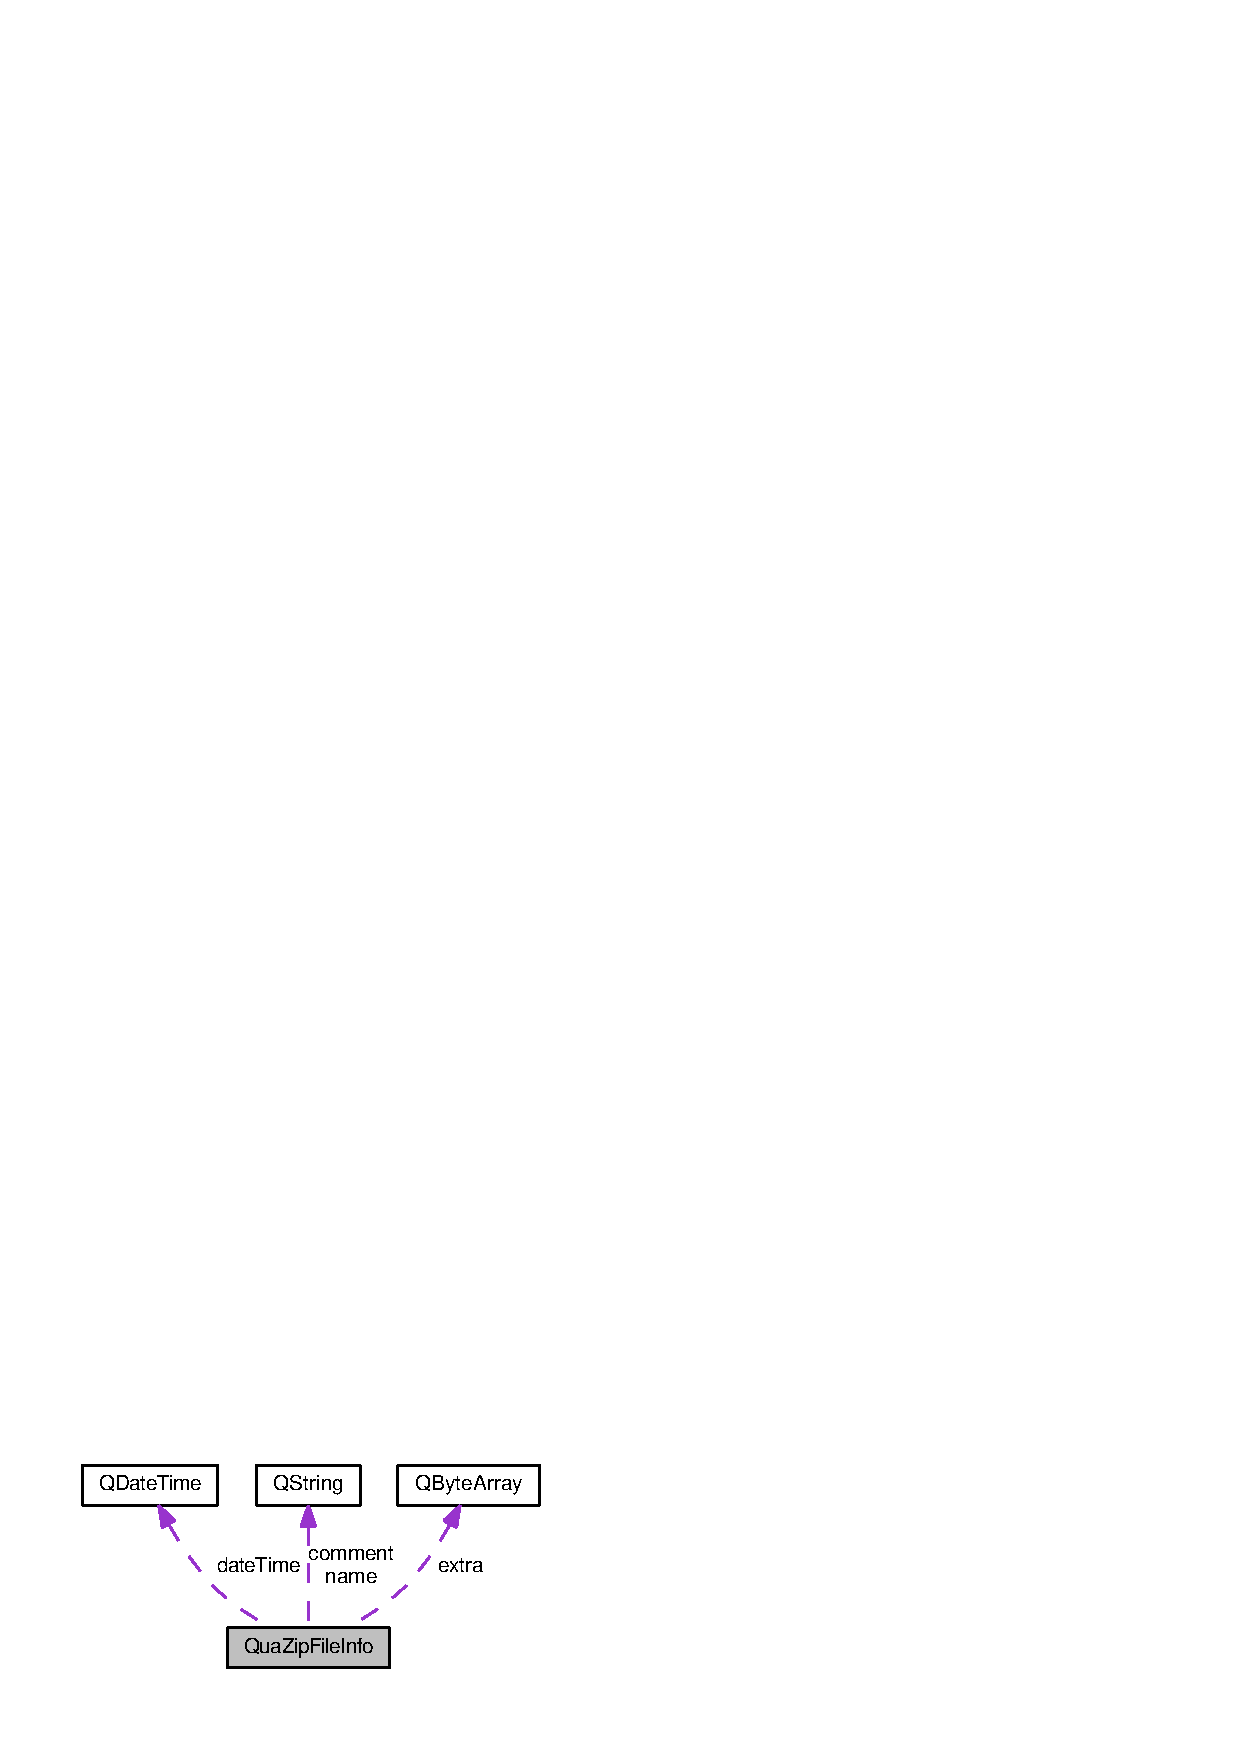
\includegraphics[width=263pt]{structQuaZipFileInfo__coll__graph}
\end{center}
\end{figure}
\subsection*{Public Member Functions}
\begin{DoxyCompactItemize}
\item 
{\bf QFile::Permissions} {\bf getPermissions} () const 
\begin{DoxyCompactList}\small\item\em Get the file permissions. \end{DoxyCompactList}\end{DoxyCompactItemize}
\subsection*{Public Attributes}
\begin{DoxyCompactItemize}
\item 
{\bf QString} {\bf name}\label{structQuaZipFileInfo_a16ac323965deccf0232bfae69d933a84}

\begin{DoxyCompactList}\small\item\em File name. \end{DoxyCompactList}\item 
quint16 {\bf versionCreated}\label{structQuaZipFileInfo_a52f3f1d960ebaa2acbc2a86458fa3e6e}

\begin{DoxyCompactList}\small\item\em Version created by. \end{DoxyCompactList}\item 
quint16 {\bf versionNeeded}\label{structQuaZipFileInfo_a8b73982808bded49e88e624a65e1a94f}

\begin{DoxyCompactList}\small\item\em Version needed to extract. \end{DoxyCompactList}\item 
quint16 {\bf flags}\label{structQuaZipFileInfo_a56d36f777e4fc892c71e22d080622e2c}

\begin{DoxyCompactList}\small\item\em General purpose flags. \end{DoxyCompactList}\item 
quint16 {\bf method}\label{structQuaZipFileInfo_af5c1bbda7f5dec2c358e7a543564de4c}

\begin{DoxyCompactList}\small\item\em Compression method. \end{DoxyCompactList}\item 
{\bf QDateTime} {\bf dateTime}\label{structQuaZipFileInfo_ad6993d099436813a27fd31aebe42911a}

\begin{DoxyCompactList}\small\item\em Last modification date and time. \end{DoxyCompactList}\item 
quint32 {\bf crc}\label{structQuaZipFileInfo_aceee045c9ebce0b9724f40d342bc99ea}

\begin{DoxyCompactList}\small\item\em CRC. \end{DoxyCompactList}\item 
quint32 {\bf compressedSize}\label{structQuaZipFileInfo_af6116eaac1f36b2a4b3a6a39851a85cc}

\begin{DoxyCompactList}\small\item\em Compressed file size. \end{DoxyCompactList}\item 
quint32 {\bf uncompressedSize}\label{structQuaZipFileInfo_a0eb908e1b1ea637d1f1f4d6aa31db07f}

\begin{DoxyCompactList}\small\item\em Uncompressed file size. \end{DoxyCompactList}\item 
quint16 {\bf diskNumberStart}\label{structQuaZipFileInfo_aa70157fdc2bd8de10405055b4233050b}

\begin{DoxyCompactList}\small\item\em Disk number start. \end{DoxyCompactList}\item 
quint16 {\bf internalAttr}\label{structQuaZipFileInfo_a36e681a93b041617addee78cb939c93d}

\begin{DoxyCompactList}\small\item\em Internal file attributes. \end{DoxyCompactList}\item 
quint32 {\bf externalAttr}\label{structQuaZipFileInfo_afeb65ffdacc4fc0ba7848d4b37f62ecf}

\begin{DoxyCompactList}\small\item\em External file attributes. \end{DoxyCompactList}\item 
{\bf QString} {\bf comment}\label{structQuaZipFileInfo_adc2aad7bbd87ce3415e2a19851266bfc}

\begin{DoxyCompactList}\small\item\em Comment. \end{DoxyCompactList}\item 
{\bf QByteArray} {\bf extra}\label{structQuaZipFileInfo_affc7b097de2c3c2ef5801c60f96adc72}

\begin{DoxyCompactList}\small\item\em Extra field. \end{DoxyCompactList}\end{DoxyCompactItemize}


\subsection{Detailed Description}
Information about a file inside archive. 

\begin{Desc}
\item[{\bf Deprecated}]Use \doxyref{QuaZipFileInfo64}{p.}{structQuaZipFileInfo64} instead. Not only it supports large files, but also more convenience methods as well.\end{Desc}


Call \doxyref{QuaZip::getCurrentFileInfo()}{p.}{classQuaZip_a9c91a53ed4c2038e153c64bdc097ebe8} or \doxyref{QuaZipFile::getFileInfo()}{p.}{classQuaZipFile_ad3f5807329321be21b12c1ba5798b359} to fill this structure. 

\subsection{Member Function Documentation}
\index{QuaZipFileInfo@{QuaZipFileInfo}!getPermissions@{getPermissions}}
\index{getPermissions@{getPermissions}!QuaZipFileInfo@{QuaZipFileInfo}}
\subsubsection[{getPermissions}]{\setlength{\rightskip}{0pt plus 5cm}{\bf QFile::Permissions} QuaZipFileInfo::getPermissions (
\begin{DoxyParamCaption}
{}
\end{DoxyParamCaption}
) const}\label{structQuaZipFileInfo_af87f96a64d7c02b002622f81d13accdb}


Get the file permissions. 

Returns the high 16 bits of external attributes converted to {\bf QFile::Permissions}. 

The documentation for this struct was generated from the following files:\begin{DoxyCompactItemize}
\item 
quazip/quazipfileinfo.h\item 
quazip/quazipfileinfo.cpp\end{DoxyCompactItemize}

\section{QuaZipFileInfo64 Struct Reference}
\label{structQuaZipFileInfo64}\index{QuaZipFileInfo64@{QuaZipFileInfo64}}


Information about a file inside archive (with zip64 support).  




{\ttfamily \#include $<$quazipfileinfo.h$>$}



Collaboration diagram for QuaZipFileInfo64:
\nopagebreak
\begin{figure}[H]
\begin{center}
\leavevmode
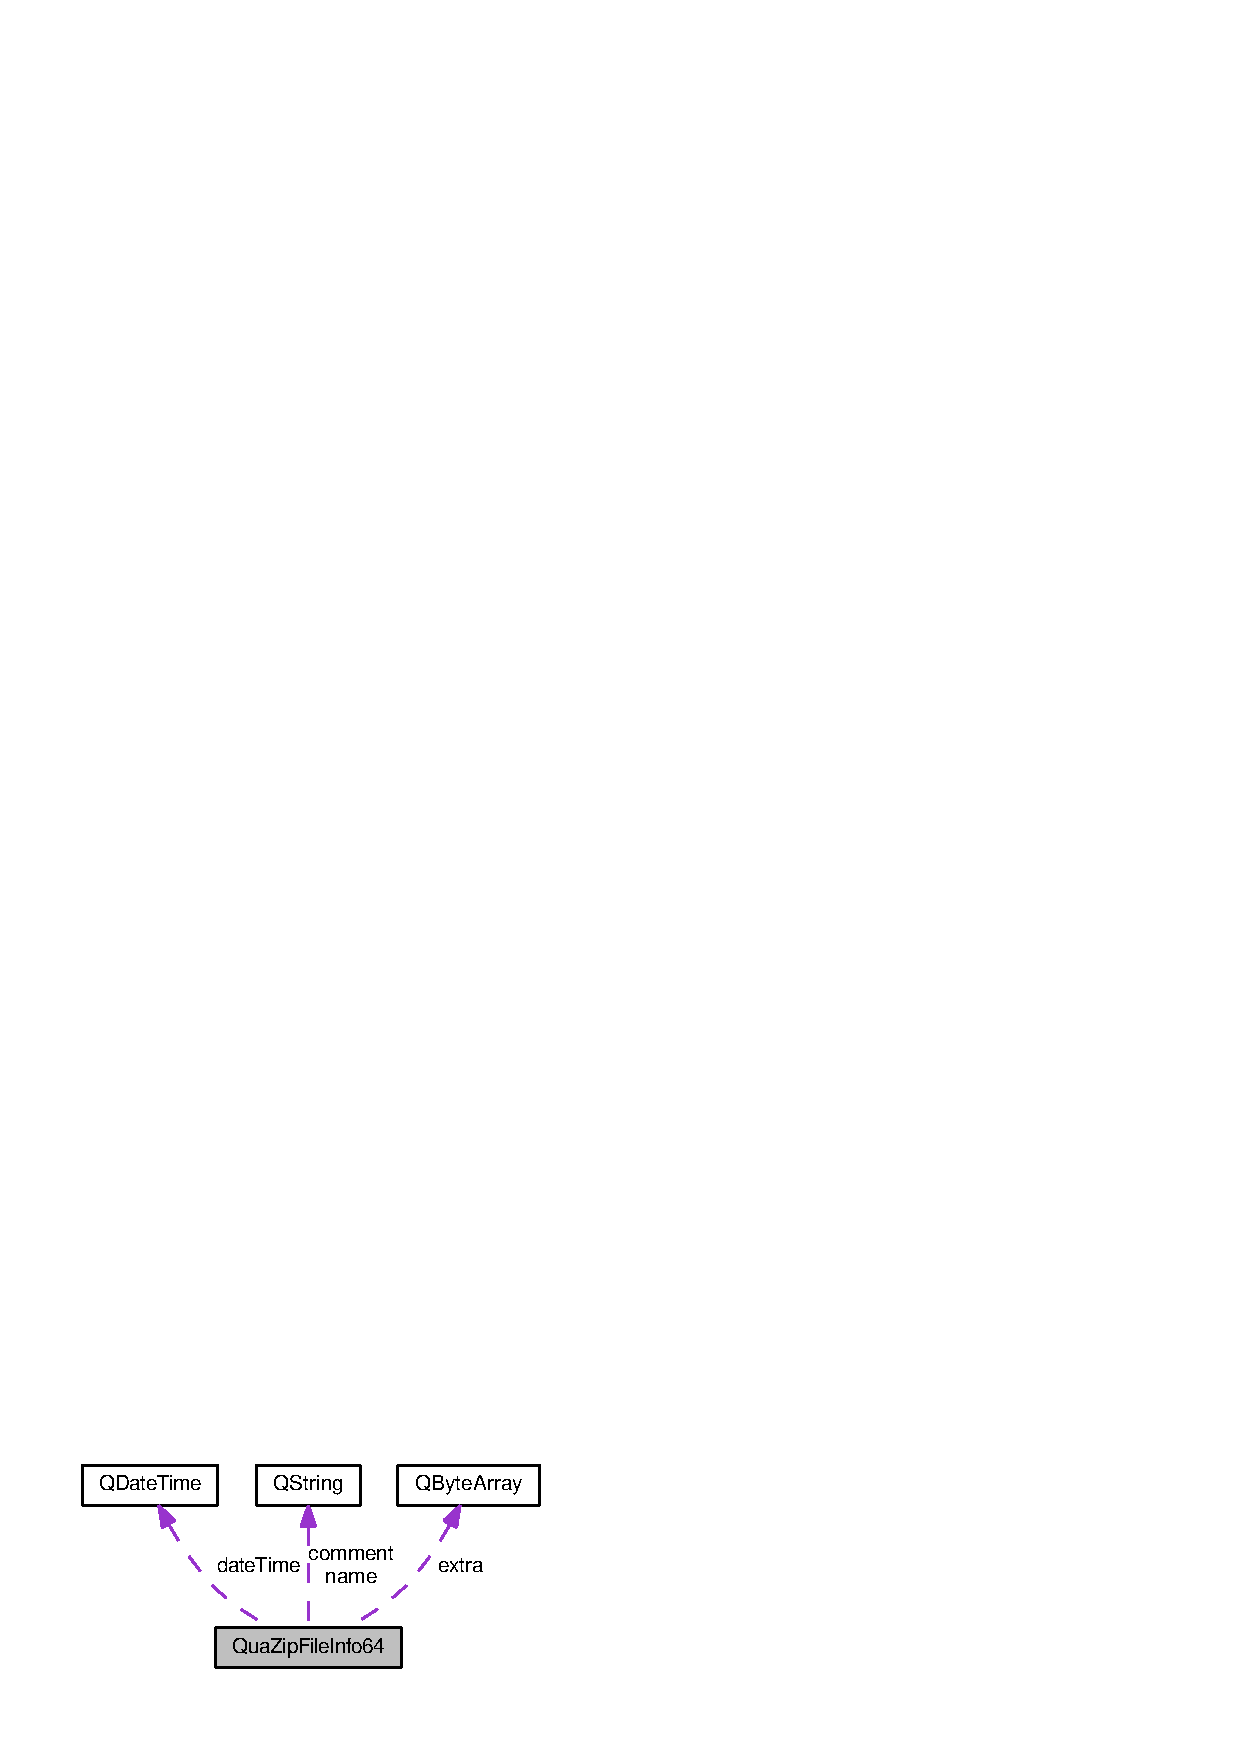
\includegraphics[width=263pt]{structQuaZipFileInfo64__coll__graph}
\end{center}
\end{figure}
\subsection*{Public Member Functions}
\begin{DoxyCompactItemize}
\item 
{\bf QFile::Permissions} {\bf getPermissions} () const 
\begin{DoxyCompactList}\small\item\em Get the file permissions. \end{DoxyCompactList}\item 
bool {\bf toQuaZipFileInfo} ({\bf QuaZipFileInfo} \&info) const 
\begin{DoxyCompactList}\small\item\em Converts to \doxyref{QuaZipFileInfo}{p.}{structQuaZipFileInfo}. \end{DoxyCompactList}\item 
{\bf QDateTime} {\bf getNTFSmTime} (int $\ast$fineTicks=NULL) const 
\begin{DoxyCompactList}\small\item\em Returns the NTFS modification time. \end{DoxyCompactList}\item 
{\bf QDateTime} {\bf getNTFSaTime} (int $\ast$fineTicks=NULL) const 
\begin{DoxyCompactList}\small\item\em Returns the NTFS access time. \end{DoxyCompactList}\item 
{\bf QDateTime} {\bf getNTFScTime} (int $\ast$fineTicks=NULL) const 
\begin{DoxyCompactList}\small\item\em Returns the NTFS creation time. \end{DoxyCompactList}\item 
bool {\bf isEncrypted} () const \label{structQuaZipFileInfo64_a8c93235e4a13ee5461023a5f3fe03e26}

\begin{DoxyCompactList}\small\item\em Checks whether the file is encrypted. \end{DoxyCompactList}\end{DoxyCompactItemize}
\subsection*{Public Attributes}
\begin{DoxyCompactItemize}
\item 
{\bf QString} {\bf name}\label{structQuaZipFileInfo64_a2cadad4cb9a765e90b5422dae2388762}

\begin{DoxyCompactList}\small\item\em File name. \end{DoxyCompactList}\item 
quint16 {\bf versionCreated}\label{structQuaZipFileInfo64_a95aeb06b080e483fde874ba2d06f203c}

\begin{DoxyCompactList}\small\item\em Version created by. \end{DoxyCompactList}\item 
quint16 {\bf versionNeeded}\label{structQuaZipFileInfo64_a27654f5ce3a75331e9c9a7900b407169}

\begin{DoxyCompactList}\small\item\em Version needed to extract. \end{DoxyCompactList}\item 
quint16 {\bf flags}\label{structQuaZipFileInfo64_a6aa533dd4e02f52459e1e1a0df31e992}

\begin{DoxyCompactList}\small\item\em General purpose flags. \end{DoxyCompactList}\item 
quint16 {\bf method}\label{structQuaZipFileInfo64_a445967ecbb5a3dd2a9d516db3e14a34a}

\begin{DoxyCompactList}\small\item\em Compression method. \end{DoxyCompactList}\item 
{\bf QDateTime} {\bf dateTime}
\begin{DoxyCompactList}\small\item\em Last modification date and time. \end{DoxyCompactList}\item 
quint32 {\bf crc}\label{structQuaZipFileInfo64_aeb7b2757a0efa814b196b5280d000a14}

\begin{DoxyCompactList}\small\item\em CRC. \end{DoxyCompactList}\item 
quint64 {\bf compressedSize}\label{structQuaZipFileInfo64_add8733946ea4af23aa32d85f10955b0f}

\begin{DoxyCompactList}\small\item\em Compressed file size. \end{DoxyCompactList}\item 
quint64 {\bf uncompressedSize}\label{structQuaZipFileInfo64_a571ca077fe282c908e57b0bc82528d49}

\begin{DoxyCompactList}\small\item\em Uncompressed file size. \end{DoxyCompactList}\item 
quint16 {\bf diskNumberStart}\label{structQuaZipFileInfo64_ac8945cf1ff54d39d28e755685b91e941}

\begin{DoxyCompactList}\small\item\em Disk number start. \end{DoxyCompactList}\item 
quint16 {\bf internalAttr}\label{structQuaZipFileInfo64_aeb895613e76a4cc63f861b010c9e92c0}

\begin{DoxyCompactList}\small\item\em Internal file attributes. \end{DoxyCompactList}\item 
quint32 {\bf externalAttr}\label{structQuaZipFileInfo64_a3a8bc40f1aa0cb0985c4e2f8a9678430}

\begin{DoxyCompactList}\small\item\em External file attributes. \end{DoxyCompactList}\item 
{\bf QString} {\bf comment}\label{structQuaZipFileInfo64_aba3f5b982087c3e0343bb61e8814c7d1}

\begin{DoxyCompactList}\small\item\em Comment. \end{DoxyCompactList}\item 
{\bf QByteArray} {\bf extra}\label{structQuaZipFileInfo64_acf0b1b97f377208847c6912cd1bf1332}

\begin{DoxyCompactList}\small\item\em Extra field. \end{DoxyCompactList}\end{DoxyCompactItemize}


\subsection{Detailed Description}
Information about a file inside archive (with zip64 support). 

Call \doxyref{QuaZip::getCurrentFileInfo()}{p.}{classQuaZip_a9c91a53ed4c2038e153c64bdc097ebe8} or \doxyref{QuaZipFile::getFileInfo()}{p.}{classQuaZipFile_ad3f5807329321be21b12c1ba5798b359} to fill this structure. 

\subsection{Member Function Documentation}
\index{QuaZipFileInfo64@{QuaZipFileInfo64}!getPermissions@{getPermissions}}
\index{getPermissions@{getPermissions}!QuaZipFileInfo64@{QuaZipFileInfo64}}
\subsubsection[{getPermissions}]{\setlength{\rightskip}{0pt plus 5cm}{\bf QFile::Permissions} QuaZipFileInfo64::getPermissions (
\begin{DoxyParamCaption}
{}
\end{DoxyParamCaption}
) const}\label{structQuaZipFileInfo64_a099216bd8991a983168d91c06a689f61}


Get the file permissions. 

Returns the high 16 bits of external attributes converted to {\bf QFile::Permissions}. \index{QuaZipFileInfo64@{QuaZipFileInfo64}!toQuaZipFileInfo@{toQuaZipFileInfo}}
\index{toQuaZipFileInfo@{toQuaZipFileInfo}!QuaZipFileInfo64@{QuaZipFileInfo64}}
\subsubsection[{toQuaZipFileInfo}]{\setlength{\rightskip}{0pt plus 5cm}bool QuaZipFileInfo64::toQuaZipFileInfo (
\begin{DoxyParamCaption}
\item[{{\bf QuaZipFileInfo} \&}]{info}
\end{DoxyParamCaption}
) const}\label{structQuaZipFileInfo64_ada29945c7ee4c9df6fbe95864793aade}


Converts to \doxyref{QuaZipFileInfo}{p.}{structQuaZipFileInfo}. 

If any of the fields are greater than 0xFFFFFFFFu, they are set to 0xFFFFFFFFu exactly, not just truncated. This function should be mainly used for compatibility with the old code expecting \doxyref{QuaZipFileInfo}{p.}{structQuaZipFileInfo}, in the cases when it's impossible or otherwise unadvisable (due to ABI compatibility reasons, for example) to modify that old code to use \doxyref{QuaZipFileInfo64}{p.}{structQuaZipFileInfo64}.

\begin{DoxyReturn}{Returns}
{\ttfamily true} if all fields converted correctly, {\ttfamily false} if an overflow occured. 
\end{DoxyReturn}


References comment, QuaZipFileInfo::comment, QuaZipFileInfo::compressedSize, compressedSize, crc, QuaZipFileInfo::crc, dateTime, QuaZipFileInfo::dateTime, diskNumberStart, QuaZipFileInfo::diskNumberStart, externalAttr, QuaZipFileInfo::externalAttr, extra, QuaZipFileInfo::extra, flags, QuaZipFileInfo::flags, internalAttr, QuaZipFileInfo::internalAttr, method, QuaZipFileInfo::method, name, QuaZipFileInfo::name, QuaZipFileInfo::uncompressedSize, uncompressedSize, versionCreated, QuaZipFileInfo::versionCreated, versionNeeded, and QuaZipFileInfo::versionNeeded.



Referenced by QuaZip::getCurrentFileInfo(), and QuaZipFile::getFileInfo().

\index{QuaZipFileInfo64@{QuaZipFileInfo64}!getNTFSmTime@{getNTFSmTime}}
\index{getNTFSmTime@{getNTFSmTime}!QuaZipFileInfo64@{QuaZipFileInfo64}}
\subsubsection[{getNTFSmTime}]{\setlength{\rightskip}{0pt plus 5cm}{\bf QDateTime} QuaZipFileInfo64::getNTFSmTime (
\begin{DoxyParamCaption}
\item[{int $\ast$}]{fineTicks = {\ttfamily NULL}}
\end{DoxyParamCaption}
) const}\label{structQuaZipFileInfo64_af4b19399367cf5bf24026344e0631ccb}


Returns the NTFS modification time. 

The getNTFS$\ast$Time() functions only work if there is an NTFS extra field present. Otherwise, they all return invalid null timestamps. 
\begin{DoxyParams}{Parameters}
{\em fineTicks} & If not NULL, the fractional part of milliseconds returned there, measured in 100-\/nanosecond ticks. Will be set to zero if there is no NTFS extra field. \\
\hline
\end{DoxyParams}
\begin{DoxySeeAlso}{See also}
\doxyref{dateTime}{p.}{structQuaZipFileInfo64_a4d77c6aa6076703e858c938efeb551e4} 

\doxyref{getNTFSaTime()}{p.}{structQuaZipFileInfo64_afe4c454de7d067a0095da0223f0cbec2} 

\doxyref{getNTFScTime()}{p.}{structQuaZipFileInfo64_a409dcbbe1ecd88dadb51be1aec48819d} 
\end{DoxySeeAlso}
\begin{DoxyReturn}{Returns}
The NTFS modification time, UTC 
\end{DoxyReturn}
\index{QuaZipFileInfo64@{QuaZipFileInfo64}!getNTFSaTime@{getNTFSaTime}}
\index{getNTFSaTime@{getNTFSaTime}!QuaZipFileInfo64@{QuaZipFileInfo64}}
\subsubsection[{getNTFSaTime}]{\setlength{\rightskip}{0pt plus 5cm}{\bf QDateTime} QuaZipFileInfo64::getNTFSaTime (
\begin{DoxyParamCaption}
\item[{int $\ast$}]{fineTicks = {\ttfamily NULL}}
\end{DoxyParamCaption}
) const}\label{structQuaZipFileInfo64_afe4c454de7d067a0095da0223f0cbec2}


Returns the NTFS access time. 

The getNTFS$\ast$Time() functions only work if there is an NTFS extra field present. Otherwise, they all return invalid null timestamps. 
\begin{DoxyParams}{Parameters}
{\em fineTicks} & If not NULL, the fractional part of milliseconds returned there, measured in 100-\/nanosecond ticks. Will be set to zero if there is no NTFS extra field. \\
\hline
\end{DoxyParams}
\begin{DoxySeeAlso}{See also}
\doxyref{dateTime}{p.}{structQuaZipFileInfo64_a4d77c6aa6076703e858c938efeb551e4} 

\doxyref{getNTFSmTime()}{p.}{structQuaZipFileInfo64_af4b19399367cf5bf24026344e0631ccb} 

\doxyref{getNTFScTime()}{p.}{structQuaZipFileInfo64_a409dcbbe1ecd88dadb51be1aec48819d} 
\end{DoxySeeAlso}
\begin{DoxyReturn}{Returns}
The NTFS access time, UTC 
\end{DoxyReturn}
\index{QuaZipFileInfo64@{QuaZipFileInfo64}!getNTFScTime@{getNTFScTime}}
\index{getNTFScTime@{getNTFScTime}!QuaZipFileInfo64@{QuaZipFileInfo64}}
\subsubsection[{getNTFScTime}]{\setlength{\rightskip}{0pt plus 5cm}{\bf QDateTime} QuaZipFileInfo64::getNTFScTime (
\begin{DoxyParamCaption}
\item[{int $\ast$}]{fineTicks = {\ttfamily NULL}}
\end{DoxyParamCaption}
) const}\label{structQuaZipFileInfo64_a409dcbbe1ecd88dadb51be1aec48819d}


Returns the NTFS creation time. 

The getNTFS$\ast$Time() functions only work if there is an NTFS extra field present. Otherwise, they all return invalid null timestamps. 
\begin{DoxyParams}{Parameters}
{\em fineTicks} & If not NULL, the fractional part of milliseconds returned there, measured in 100-\/nanosecond ticks. Will be set to zero if there is no NTFS extra field. \\
\hline
\end{DoxyParams}
\begin{DoxySeeAlso}{See also}
\doxyref{dateTime}{p.}{structQuaZipFileInfo64_a4d77c6aa6076703e858c938efeb551e4} 

\doxyref{getNTFSmTime()}{p.}{structQuaZipFileInfo64_af4b19399367cf5bf24026344e0631ccb} 

\doxyref{getNTFSaTime()}{p.}{structQuaZipFileInfo64_afe4c454de7d067a0095da0223f0cbec2} 
\end{DoxySeeAlso}
\begin{DoxyReturn}{Returns}
The NTFS creation time, UTC 
\end{DoxyReturn}


\subsection{Member Data Documentation}
\index{QuaZipFileInfo64@{QuaZipFileInfo64}!dateTime@{dateTime}}
\index{dateTime@{dateTime}!QuaZipFileInfo64@{QuaZipFileInfo64}}
\subsubsection[{dateTime}]{\setlength{\rightskip}{0pt plus 5cm}{\bf QDateTime} {\bf QuaZipFileInfo64::dateTime}}\label{structQuaZipFileInfo64_a4d77c6aa6076703e858c938efeb551e4}


Last modification date and time. 

This is the time stored in the standard ZIP header. This format only allows to store time with 2-\/second precision, so the seconds will always be even and the milliseconds will always be zero. If you need more precise date and time, you can try to call the \doxyref{getNTFSmTime()}{p.}{structQuaZipFileInfo64_af4b19399367cf5bf24026344e0631ccb} function or its siblings, provided that the archive itself contains these NTFS times. 

Referenced by QuaZip::getCurrentFileInfo(), and toQuaZipFileInfo().



The documentation for this struct was generated from the following files:\begin{DoxyCompactItemize}
\item 
quazip/quazipfileinfo.h\item 
quazip/quazipfileinfo.cpp\end{DoxyCompactItemize}

\section{QuaZipFilePrivate Class Reference}
\label{classQuaZipFilePrivate}\index{QuaZipFilePrivate@{QuaZipFilePrivate}}


The implementation class for \doxyref{QuaZip}{p.}{classQuaZip}.  




Collaboration diagram for QuaZipFilePrivate:
\nopagebreak
\begin{figure}[H]
\begin{center}
\leavevmode
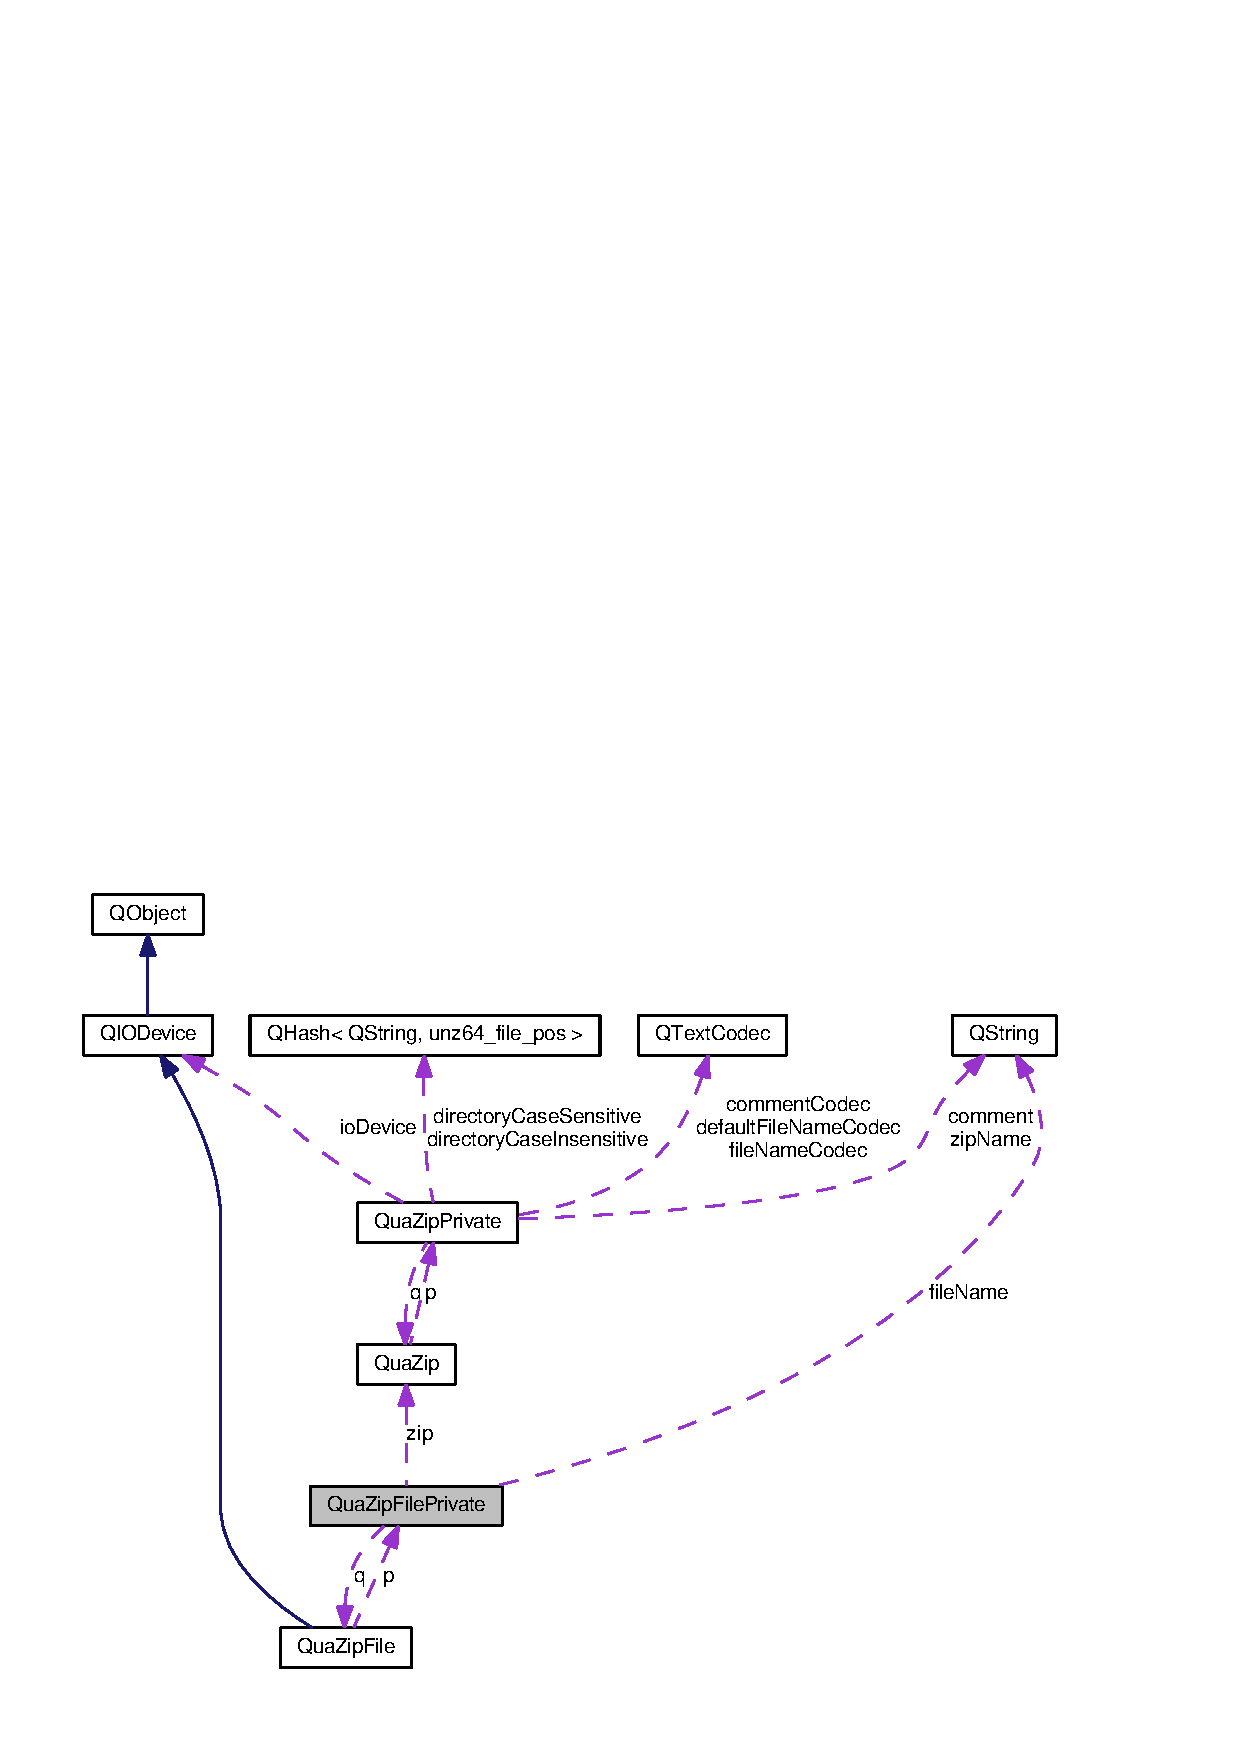
\includegraphics[width=400pt]{classQuaZipFilePrivate__coll__graph}
\end{center}
\end{figure}
\subsection*{Friends}
\begin{DoxyCompactItemize}
\item 
class {\bf QuaZipFile}\label{classQuaZipFilePrivate_a40bd4ccb6d2d00726e1de81329ebaa7a}

\end{DoxyCompactItemize}


\subsection{Detailed Description}
The implementation class for \doxyref{QuaZip}{p.}{classQuaZip}. 

The documentation for this class was generated from the following file:\begin{DoxyCompactItemize}
\item 
quazip/quazipfile.cpp\end{DoxyCompactItemize}

\section{QuaZipNewInfo Struct Reference}
\label{structQuaZipNewInfo}\index{QuaZipNewInfo@{QuaZipNewInfo}}


Information about a file to be created.  




{\ttfamily \#include $<$quazipnewinfo.h$>$}



Collaboration diagram for QuaZipNewInfo:
\nopagebreak
\begin{figure}[H]
\begin{center}
\leavevmode
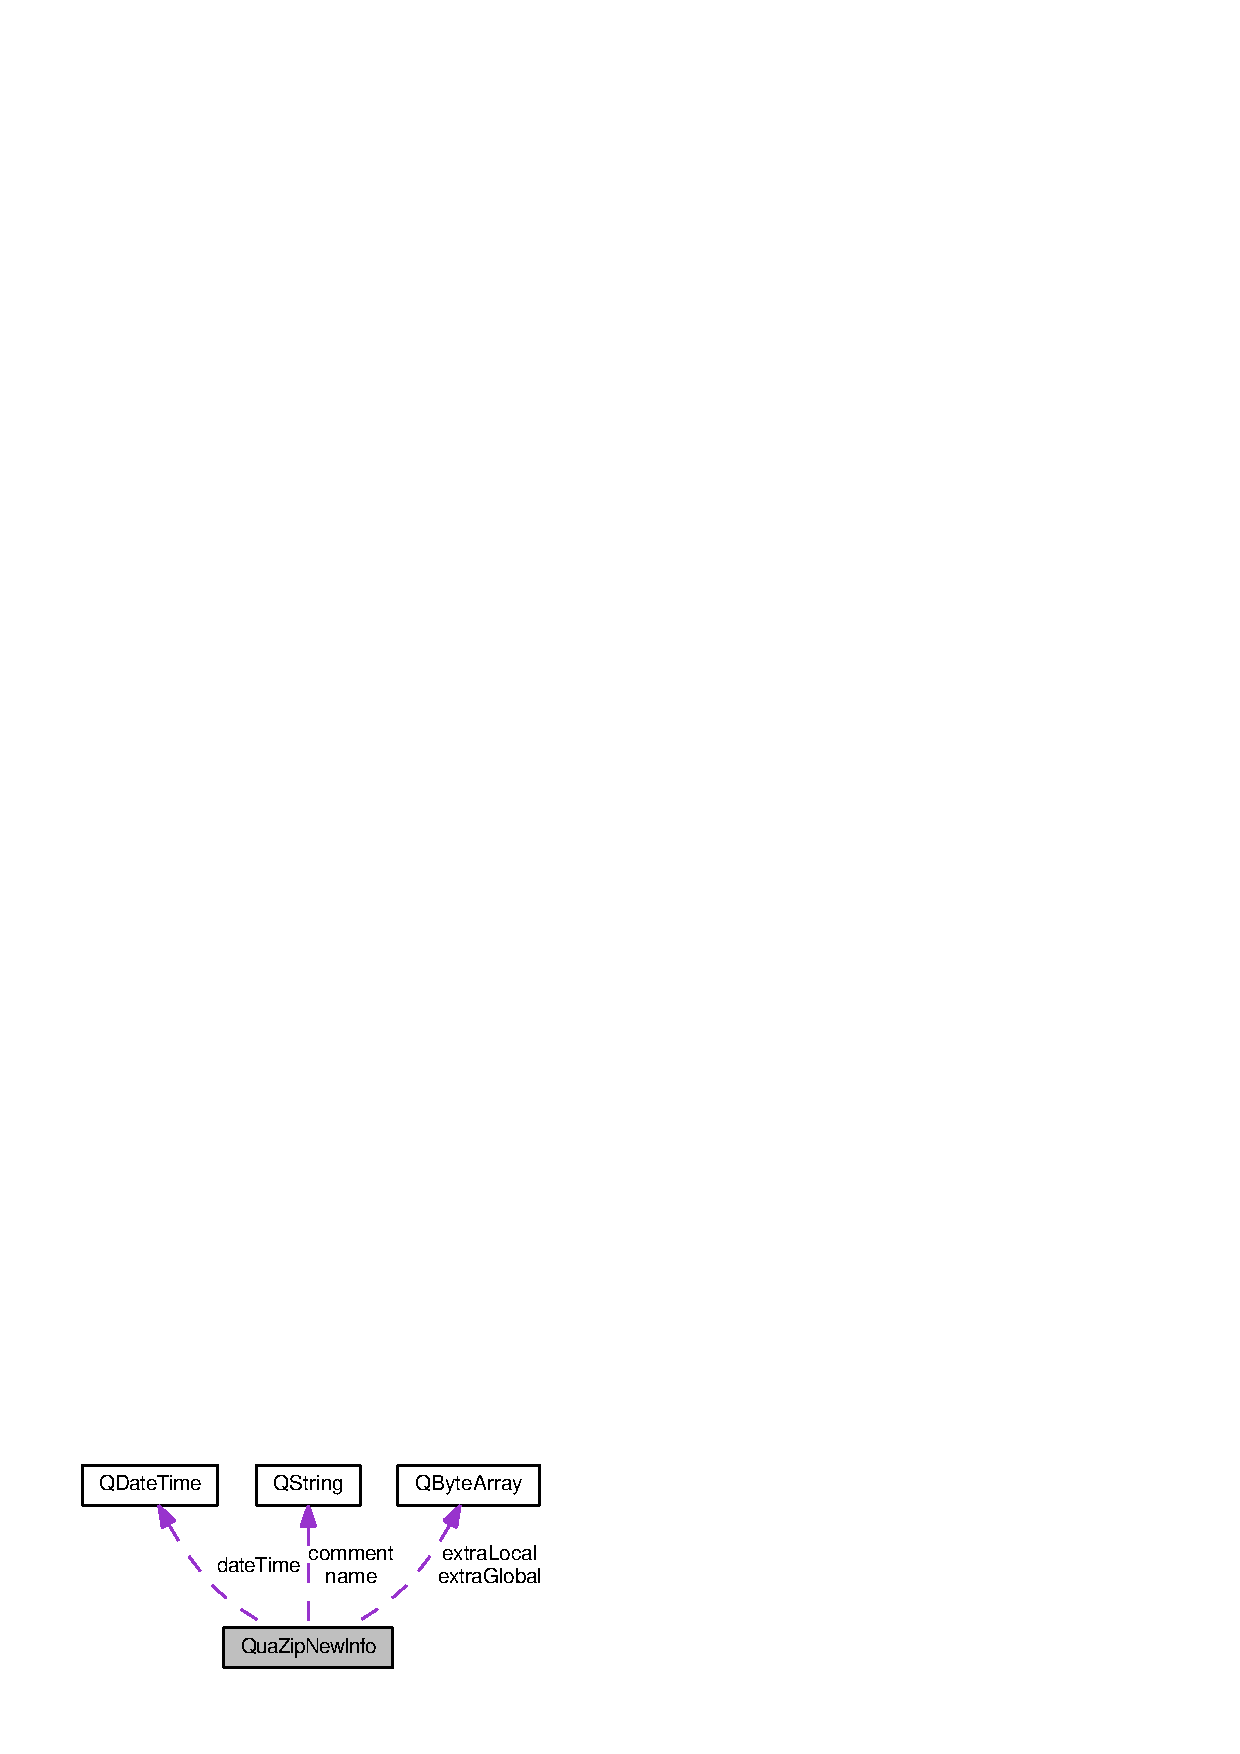
\includegraphics[width=264pt]{structQuaZipNewInfo__coll__graph}
\end{center}
\end{figure}
\subsection*{Public Member Functions}
\begin{DoxyCompactItemize}
\item 
{\bf QuaZipNewInfo} (const {\bf QString} \&{\bf name})
\begin{DoxyCompactList}\small\item\em Constructs \doxyref{QuaZipNewInfo}{p.}{structQuaZipNewInfo} instance. \end{DoxyCompactList}\item 
{\bf QuaZipNewInfo} (const {\bf QString} \&{\bf name}, const {\bf QString} \&file)
\begin{DoxyCompactList}\small\item\em Constructs \doxyref{QuaZipNewInfo}{p.}{structQuaZipNewInfo} instance. \end{DoxyCompactList}\item 
{\bf QuaZipNewInfo} (const {\bf QuaZipFileInfo} \&existing)
\begin{DoxyCompactList}\small\item\em Initializes the new instance from existing file info. \end{DoxyCompactList}\item 
{\bf QuaZipNewInfo} (const {\bf QuaZipFileInfo64} \&existing)
\begin{DoxyCompactList}\small\item\em Initializes the new instance from existing file info. \end{DoxyCompactList}\item 
void {\bf setFileDateTime} (const {\bf QString} \&file)
\begin{DoxyCompactList}\small\item\em Sets the file timestamp from the existing file. \end{DoxyCompactList}\item 
void {\bf setFilePermissions} (const {\bf QString} \&file)
\begin{DoxyCompactList}\small\item\em Sets the file permissions from the existing file. \end{DoxyCompactList}\item 
void {\bf setPermissions} ({\bf QFile::Permissions} permissions)
\begin{DoxyCompactList}\small\item\em Sets the file permissions. \end{DoxyCompactList}\item 
void {\bf setFileNTFSTimes} (const {\bf QString} \&fileName)
\begin{DoxyCompactList}\small\item\em Sets the NTFS times from an existing file. \end{DoxyCompactList}\item 
void {\bf setFileNTFSmTime} (const {\bf QDateTime} \&mTime, int fineTicks=0)
\begin{DoxyCompactList}\small\item\em Sets the NTFS modification time. \end{DoxyCompactList}\item 
void {\bf setFileNTFSaTime} (const {\bf QDateTime} \&aTime, int fineTicks=0)
\begin{DoxyCompactList}\small\item\em Sets the NTFS access time. \end{DoxyCompactList}\item 
void {\bf setFileNTFScTime} (const {\bf QDateTime} \&cTime, int fineTicks=0)
\begin{DoxyCompactList}\small\item\em Sets the NTFS creation time. \end{DoxyCompactList}\end{DoxyCompactItemize}
\subsection*{Public Attributes}
\begin{DoxyCompactItemize}
\item 
{\bf QString} {\bf name}
\begin{DoxyCompactList}\small\item\em File name. \end{DoxyCompactList}\item 
{\bf QDateTime} {\bf dateTime}
\begin{DoxyCompactList}\small\item\em File timestamp. \end{DoxyCompactList}\item 
quint16 {\bf internalAttr}\label{structQuaZipNewInfo_a59ce9776c2ac7547ade8cb4c404c77ab}

\begin{DoxyCompactList}\small\item\em File internal attributes. \end{DoxyCompactList}\item 
quint32 {\bf externalAttr}
\begin{DoxyCompactList}\small\item\em File external attributes. \end{DoxyCompactList}\item 
{\bf QString} {\bf comment}
\begin{DoxyCompactList}\small\item\em File comment. \end{DoxyCompactList}\item 
{\bf QByteArray} {\bf extraLocal}\label{structQuaZipNewInfo_ab377a81c51cf495c7aeee4f19340a43f}

\begin{DoxyCompactList}\small\item\em File local extra field. \end{DoxyCompactList}\item 
{\bf QByteArray} {\bf extraGlobal}\label{structQuaZipNewInfo_abda207eb3949db3a88761c1b06e6bd58}

\begin{DoxyCompactList}\small\item\em File global extra field. \end{DoxyCompactList}\item 
ulong {\bf uncompressedSize}
\begin{DoxyCompactList}\small\item\em Uncompressed file size. \end{DoxyCompactList}\end{DoxyCompactItemize}


\subsection{Detailed Description}
Information about a file to be created. 

This structure holds information about a file to be created inside ZIP archive. At least name should be set to something correct before passing this structure to QuaZipFile::open(OpenMode,const QuaZipNewInfo\&,int,int,bool).

Zip64 support of this structure is slightly limited: in the raw mode (when a pre-\/compressed file is written into a ZIP file as-\/is), it is necessary to specify the uncompressed file size and the appropriate field is 32 bit. Since the raw mode is used extremely rare, there is no real need to have a separate QuaZipNewInfo64 structure like \doxyref{QuaZipFileInfo64}{p.}{structQuaZipFileInfo64}. It may be added in the future though, if there is a demand for the raw mode with zip64 archives. 

\subsection{Constructor \& Destructor Documentation}
\index{QuaZipNewInfo@{QuaZipNewInfo}!QuaZipNewInfo@{QuaZipNewInfo}}
\index{QuaZipNewInfo@{QuaZipNewInfo}!QuaZipNewInfo@{QuaZipNewInfo}}
\subsubsection[{QuaZipNewInfo}]{\setlength{\rightskip}{0pt plus 5cm}QuaZipNewInfo::QuaZipNewInfo (
\begin{DoxyParamCaption}
\item[{const {\bf QString} \&}]{name}
\end{DoxyParamCaption}
)}\label{structQuaZipNewInfo_a46c0f551cf9e6b2131929beb39187aac}


Constructs \doxyref{QuaZipNewInfo}{p.}{structQuaZipNewInfo} instance. 

Initializes name with {\itshape name\/}, dateTime with current date and time. Attributes are initialized with zeros, comment and extra field with null values. \index{QuaZipNewInfo@{QuaZipNewInfo}!QuaZipNewInfo@{QuaZipNewInfo}}
\index{QuaZipNewInfo@{QuaZipNewInfo}!QuaZipNewInfo@{QuaZipNewInfo}}
\subsubsection[{QuaZipNewInfo}]{\setlength{\rightskip}{0pt plus 5cm}QuaZipNewInfo::QuaZipNewInfo (
\begin{DoxyParamCaption}
\item[{const {\bf QString} \&}]{name, }
\item[{const {\bf QString} \&}]{file}
\end{DoxyParamCaption}
)}\label{structQuaZipNewInfo_ad47cf11f4277edcb09a8ba2b2963f2a9}


Constructs \doxyref{QuaZipNewInfo}{p.}{structQuaZipNewInfo} instance. 

Initializes name with {\itshape name\/}. Timestamp and permissions are taken from the specified file. If the {\itshape file\/} does not exists or its timestamp is inaccessible (e. g. you do not have read permission for the directory file in), uses current time and zero permissions. Other attributes are initialized with zeros, comment and extra field with null values.

\begin{DoxySeeAlso}{See also}
\doxyref{setFileDateTime()}{p.}{structQuaZipNewInfo_a2b18b554d056877a2f33ffb9d241ed85} 
\end{DoxySeeAlso}


References QDateTime::currentDateTime(), dateTime, QFileInfo::exists(), QFileInfo::isDir(), QFileInfo::lastModified(), and QFileInfo::permissions().

\index{QuaZipNewInfo@{QuaZipNewInfo}!QuaZipNewInfo@{QuaZipNewInfo}}
\index{QuaZipNewInfo@{QuaZipNewInfo}!QuaZipNewInfo@{QuaZipNewInfo}}
\subsubsection[{QuaZipNewInfo}]{\setlength{\rightskip}{0pt plus 5cm}QuaZipNewInfo::QuaZipNewInfo (
\begin{DoxyParamCaption}
\item[{const {\bf QuaZipFileInfo} \&}]{existing}
\end{DoxyParamCaption}
)}\label{structQuaZipNewInfo_a5f1a867f3b0d29d076f9014f70b59e5a}


Initializes the new instance from existing file info. 

Mainly used when copying files between archives.

Both extra fields are initialized to existing.extra. \doxyref{QuaZipNewInfo}{p.}{structQuaZipNewInfo} 
\begin{DoxyParams}{Parameters}
{\em existing} & \\
\hline
\end{DoxyParams}
\index{QuaZipNewInfo@{QuaZipNewInfo}!QuaZipNewInfo@{QuaZipNewInfo}}
\index{QuaZipNewInfo@{QuaZipNewInfo}!QuaZipNewInfo@{QuaZipNewInfo}}
\subsubsection[{QuaZipNewInfo}]{\setlength{\rightskip}{0pt plus 5cm}QuaZipNewInfo::QuaZipNewInfo (
\begin{DoxyParamCaption}
\item[{const {\bf QuaZipFileInfo64} \&}]{existing}
\end{DoxyParamCaption}
)}\label{structQuaZipNewInfo_a4afa2e8c282a801fc216f79026c2d062}


Initializes the new instance from existing file info. 

Mainly used when copying files between archives.

Both extra fields are initialized to existing.extra. \doxyref{QuaZipNewInfo}{p.}{structQuaZipNewInfo} 
\begin{DoxyParams}{Parameters}
{\em existing} & \\
\hline
\end{DoxyParams}


\subsection{Member Function Documentation}
\index{QuaZipNewInfo@{QuaZipNewInfo}!setFileDateTime@{setFileDateTime}}
\index{setFileDateTime@{setFileDateTime}!QuaZipNewInfo@{QuaZipNewInfo}}
\subsubsection[{setFileDateTime}]{\setlength{\rightskip}{0pt plus 5cm}void QuaZipNewInfo::setFileDateTime (
\begin{DoxyParamCaption}
\item[{const {\bf QString} \&}]{file}
\end{DoxyParamCaption}
)}\label{structQuaZipNewInfo_a2b18b554d056877a2f33ffb9d241ed85}


Sets the file timestamp from the existing file. 

Use this function to set the file timestamp from the existing file. Use it like this: 
\begin{DoxyCode}
 QuaZipFile zipFile(&zip);
 QFile file("file-to-add");
 file.open(QIODevice::ReadOnly);
 QuaZipNewInfo info("file-name-in-archive");
 info.setFileDateTime("file-to-add"); // take the timestamp from file
 zipFile.open(QIODevice::WriteOnly, info);
\end{DoxyCode}


This function does not change dateTime if some error occured (e. g. file is inaccessible). 

References dateTime, QFileInfo::exists(), and QFileInfo::lastModified().

\index{QuaZipNewInfo@{QuaZipNewInfo}!setFilePermissions@{setFilePermissions}}
\index{setFilePermissions@{setFilePermissions}!QuaZipNewInfo@{QuaZipNewInfo}}
\subsubsection[{setFilePermissions}]{\setlength{\rightskip}{0pt plus 5cm}void QuaZipNewInfo::setFilePermissions (
\begin{DoxyParamCaption}
\item[{const {\bf QString} \&}]{file}
\end{DoxyParamCaption}
)}\label{structQuaZipNewInfo_a08bee5211eb0b49da260c7a9e7a266b8}


Sets the file permissions from the existing file. 

Takes permissions from the file and sets the high 16 bits of external attributes. Uses {\bf QFileInfo} to get permissions on all platforms. 

References QFileInfo::isDir(), QFileInfo::permissions(), and QFileDevice::Permissions.

\index{QuaZipNewInfo@{QuaZipNewInfo}!setPermissions@{setPermissions}}
\index{setPermissions@{setPermissions}!QuaZipNewInfo@{QuaZipNewInfo}}
\subsubsection[{setPermissions}]{\setlength{\rightskip}{0pt plus 5cm}void QuaZipNewInfo::setPermissions (
\begin{DoxyParamCaption}
\item[{{\bf QFile::Permissions}}]{permissions}
\end{DoxyParamCaption}
)}\label{structQuaZipNewInfo_aed68dc20f7dc42b5056491cf3c1d2d20}


Sets the file permissions. 

Modifies the highest 16 bits of external attributes. The type part is set to dir if the name ends with a slash, and to regular file otherwise. 

References QString::endsWith(), and name.

\index{QuaZipNewInfo@{QuaZipNewInfo}!setFileNTFSTimes@{setFileNTFSTimes}}
\index{setFileNTFSTimes@{setFileNTFSTimes}!QuaZipNewInfo@{QuaZipNewInfo}}
\subsubsection[{setFileNTFSTimes}]{\setlength{\rightskip}{0pt plus 5cm}void QuaZipNewInfo::setFileNTFSTimes (
\begin{DoxyParamCaption}
\item[{const {\bf QString} \&}]{fileName}
\end{DoxyParamCaption}
)}\label{structQuaZipNewInfo_a663a37c5a7a2d18900ba8b0199617eff}


Sets the NTFS times from an existing file. 

If the file doesn't exist, a warning is printed to the stderr and nothing is done. Otherwise, all three times, as reported by {\bf QFileInfo::lastModified()}, {\bf QFileInfo::lastRead()} and {\bf QFileInfo::created()}, are written to the NTFS extra field record.

The NTFS record is written to both the local and the global extra fields, updating the existing record if there is one, or creating a new one and appending it to the end of each extra field.

The microseconds will be zero, as they aren't reported by {\bf QFileInfo}. 
\begin{DoxyParams}{Parameters}
{\em fileName} & \\
\hline
\end{DoxyParams}


References QByteArray::constData(), QFileInfo::created(), QFileInfo::exists(), QFileInfo::lastModified(), QFileInfo::lastRead(), setFileNTFSaTime(), setFileNTFScTime(), setFileNTFSmTime(), and QString::toUtf8().

\index{QuaZipNewInfo@{QuaZipNewInfo}!setFileNTFSmTime@{setFileNTFSmTime}}
\index{setFileNTFSmTime@{setFileNTFSmTime}!QuaZipNewInfo@{QuaZipNewInfo}}
\subsubsection[{setFileNTFSmTime}]{\setlength{\rightskip}{0pt plus 5cm}void QuaZipNewInfo::setFileNTFSmTime (
\begin{DoxyParamCaption}
\item[{const {\bf QDateTime} \&}]{mTime, }
\item[{int}]{fineTicks = {\ttfamily 0}}
\end{DoxyParamCaption}
)}\label{structQuaZipNewInfo_a3af07365df1d67502ab1d0ca0d45df79}


Sets the NTFS modification time. 

The time is written into the NTFS record in both the local and the global extra fields, updating the existing record if there is one, or creating a new one and appending it to the end of each extra field. When updating an existing record, all other fields are left intact. 
\begin{DoxyParams}{Parameters}
{\em mTime} & The new modification time. \\
\hline
{\em fineTicks} & The fractional part of milliseconds, in 100-\/nanosecond ticks (i. e. 9999 ticks = 999.9 microsecond). Values greater than 9999 will add milliseconds or even seconds, but this can be confusing and therefore is discouraged. \\
\hline
\end{DoxyParams}


References extraGlobal, and extraLocal.



Referenced by setFileNTFSTimes().

\index{QuaZipNewInfo@{QuaZipNewInfo}!setFileNTFSaTime@{setFileNTFSaTime}}
\index{setFileNTFSaTime@{setFileNTFSaTime}!QuaZipNewInfo@{QuaZipNewInfo}}
\subsubsection[{setFileNTFSaTime}]{\setlength{\rightskip}{0pt plus 5cm}void QuaZipNewInfo::setFileNTFSaTime (
\begin{DoxyParamCaption}
\item[{const {\bf QDateTime} \&}]{aTime, }
\item[{int}]{fineTicks = {\ttfamily 0}}
\end{DoxyParamCaption}
)}\label{structQuaZipNewInfo_a1042ac3d55a9deed760eb357aaa8284c}


Sets the NTFS access time. 

The time is written into the NTFS record in both the local and the global extra fields, updating the existing record if there is one, or creating a new one and appending it to the end of each extra field. When updating an existing record, all other fields are left intact. 
\begin{DoxyParams}{Parameters}
{\em aTime} & The new access time. \\
\hline
{\em fineTicks} & The fractional part of milliseconds, in 100-\/nanosecond ticks (i. e. 9999 ticks = 999.9 microsecond). Values greater than 9999 will add milliseconds or even seconds, but this can be confusing and therefore is discouraged. \\
\hline
\end{DoxyParams}


References extraGlobal, and extraLocal.



Referenced by setFileNTFSTimes().

\index{QuaZipNewInfo@{QuaZipNewInfo}!setFileNTFScTime@{setFileNTFScTime}}
\index{setFileNTFScTime@{setFileNTFScTime}!QuaZipNewInfo@{QuaZipNewInfo}}
\subsubsection[{setFileNTFScTime}]{\setlength{\rightskip}{0pt plus 5cm}void QuaZipNewInfo::setFileNTFScTime (
\begin{DoxyParamCaption}
\item[{const {\bf QDateTime} \&}]{cTime, }
\item[{int}]{fineTicks = {\ttfamily 0}}
\end{DoxyParamCaption}
)}\label{structQuaZipNewInfo_a44675ac1e306eddefcaa35972c294d15}


Sets the NTFS creation time. 

The time is written into the NTFS record in both the local and the global extra fields, updating the existing record if there is one, or creating a new one and appending it to the end of each extra field. When updating an existing record, all other fields are left intact. 
\begin{DoxyParams}{Parameters}
{\em cTime} & The new creation time. \\
\hline
{\em fineTicks} & The fractional part of milliseconds, in 100-\/nanosecond ticks (i. e. 9999 ticks = 999.9 microsecond). Values greater than 9999 will add milliseconds or even seconds, but this can be confusing and therefore is discouraged. \\
\hline
\end{DoxyParams}


References extraGlobal, and extraLocal.



Referenced by setFileNTFSTimes().



\subsection{Member Data Documentation}
\index{QuaZipNewInfo@{QuaZipNewInfo}!name@{name}}
\index{name@{name}!QuaZipNewInfo@{QuaZipNewInfo}}
\subsubsection[{name}]{\setlength{\rightskip}{0pt plus 5cm}{\bf QString} {\bf QuaZipNewInfo::name}}\label{structQuaZipNewInfo_a2bdef01b6ac3326e48598e32bfa5fbe8}


File name. 

This field holds file name inside archive, including path relative to archive root. 

Referenced by QuaZipFile::open(), and setPermissions().

\index{QuaZipNewInfo@{QuaZipNewInfo}!dateTime@{dateTime}}
\index{dateTime@{dateTime}!QuaZipNewInfo@{QuaZipNewInfo}}
\subsubsection[{dateTime}]{\setlength{\rightskip}{0pt plus 5cm}{\bf QDateTime} {\bf QuaZipNewInfo::dateTime}}\label{structQuaZipNewInfo_aec7f3ac72c72a2e10b82ad64c2fa3453}


File timestamp. 

This is the last file modification date and time. Will be stored in the archive central directory. It is a good practice to set it to the source file timestamp instead of archive creating time. Use \doxyref{setFileDateTime()}{p.}{structQuaZipNewInfo_a2b18b554d056877a2f33ffb9d241ed85} or \doxyref{QuaZipNewInfo(const QString\&, const QString\&)}{p.}{structQuaZipNewInfo_ad47cf11f4277edcb09a8ba2b2963f2a9}. 

Referenced by QuaZipFile::open(), QuaZipNewInfo(), and setFileDateTime().

\index{QuaZipNewInfo@{QuaZipNewInfo}!externalAttr@{externalAttr}}
\index{externalAttr@{externalAttr}!QuaZipNewInfo@{QuaZipNewInfo}}
\subsubsection[{externalAttr}]{\setlength{\rightskip}{0pt plus 5cm}quint32 {\bf QuaZipNewInfo::externalAttr}}\label{structQuaZipNewInfo_affd1a9700d302e1395bd04f0864da7d0}


File external attributes. 

The highest 16 bits contain Unix file permissions and type (dir or file). The constructor \doxyref{QuaZipNewInfo(const QString\&, const QString\&)}{p.}{structQuaZipNewInfo_ad47cf11f4277edcb09a8ba2b2963f2a9} takes permissions from the provided file. 

Referenced by QuaZipFile::open().

\index{QuaZipNewInfo@{QuaZipNewInfo}!comment@{comment}}
\index{comment@{comment}!QuaZipNewInfo@{QuaZipNewInfo}}
\subsubsection[{comment}]{\setlength{\rightskip}{0pt plus 5cm}{\bf QString} {\bf QuaZipNewInfo::comment}}\label{structQuaZipNewInfo_ae24b1d38c3550b4724862ffcf8f20924}


File comment. 

Will be encoded using \doxyref{QuaZip::getCommentCodec()}{p.}{classQuaZip_a008260161781d8b5d2a0a28493fddaf4}. 

Referenced by QuaZipFile::open().

\index{QuaZipNewInfo@{QuaZipNewInfo}!uncompressedSize@{uncompressedSize}}
\index{uncompressedSize@{uncompressedSize}!QuaZipNewInfo@{QuaZipNewInfo}}
\subsubsection[{uncompressedSize}]{\setlength{\rightskip}{0pt plus 5cm}ulong {\bf QuaZipNewInfo::uncompressedSize}}\label{structQuaZipNewInfo_a18c079b3f2f5ab6eecdd61d6dbe93be6}


Uncompressed file size. 

This is only needed if you are using raw file zipping mode, i. e. adding precompressed file in the zip archive. 

Referenced by QuaZipFile::open().



The documentation for this struct was generated from the following files:\begin{DoxyCompactItemize}
\item 
quazip/quazipnewinfo.h\item 
quazip/quazipnewinfo.cpp\end{DoxyCompactItemize}

\section{QuaZipPrivate Class Reference}
\label{classQuaZipPrivate}\index{QuaZipPrivate@{QuaZipPrivate}}


All the internal stuff for the \doxyref{QuaZip}{p.}{classQuaZip} class.  




Collaboration diagram for QuaZipPrivate:
\nopagebreak
\begin{figure}[H]
\begin{center}
\leavevmode
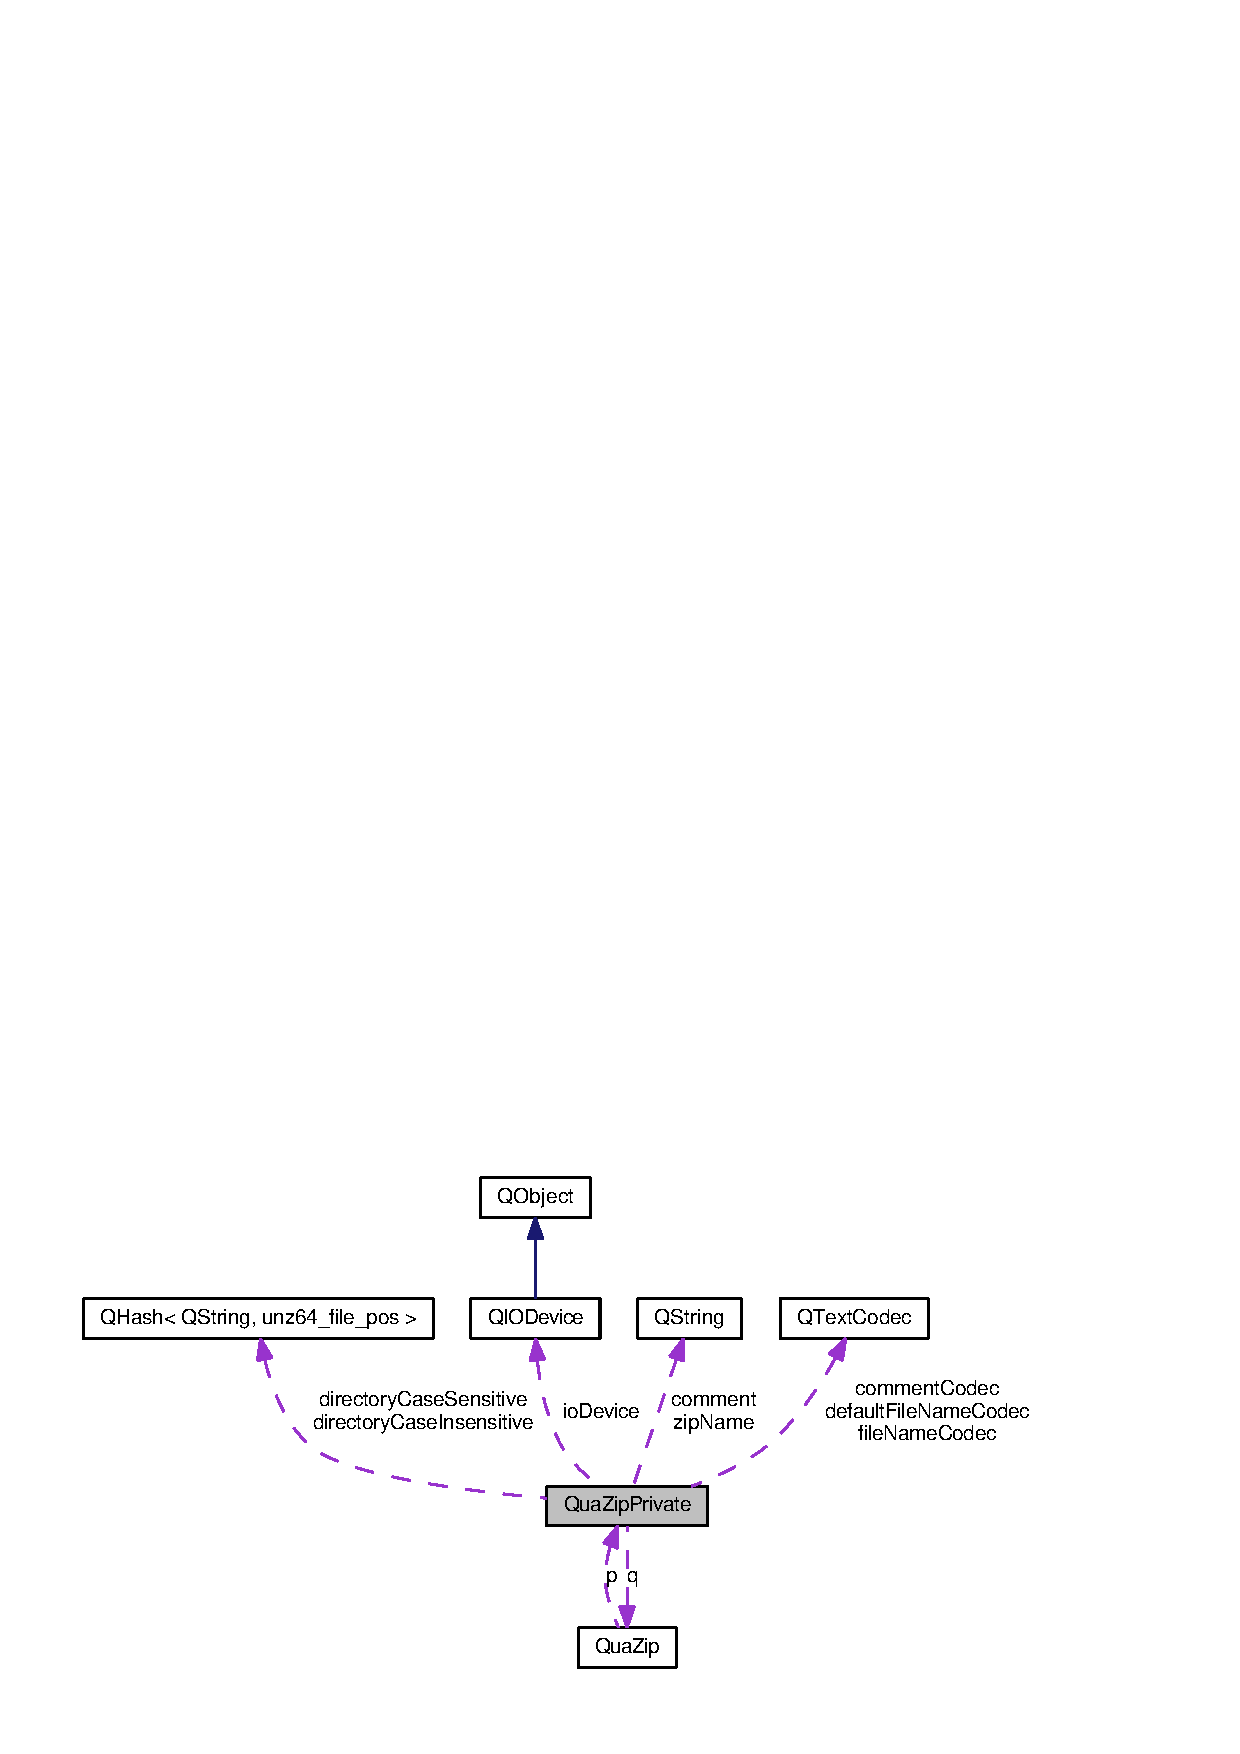
\includegraphics[width=400pt]{classQuaZipPrivate__coll__graph}
\end{center}
\end{figure}
\subsection*{Friends}
\begin{DoxyCompactItemize}
\item 
class {\bf QuaZip}\label{classQuaZipPrivate_a913fb7bbd3527119ebb8052d57132af2}

\end{DoxyCompactItemize}


\subsection{Detailed Description}
All the internal stuff for the \doxyref{QuaZip}{p.}{classQuaZip} class. 

The documentation for this class was generated from the following file:\begin{DoxyCompactItemize}
\item 
quazip/quazip.cpp\end{DoxyCompactItemize}

\printindex
\end{document}
